\chapter{Production II: Individual variability in the encoding of lexical and referential givenness, grammatical role, and sentence position} \label{ch:Production II}
\chaptermark{Production study II}

\section{Overview}

In this chapter, we investigate inter-individual variability in the prosodic encoding of lexical and referential givenness (or information status) as well as the syntactic factors grammatical role and sentence position. Building on the findings of the first production experiment presented in Chapter \ref{ch:Production I}, the present study thus considers more factors that influence prominence production and are potentially marked differently across speakers. Using a similar method as in the first study, we scrutinize the extent and form of individual variability in production data collected in an interactive reading task. In addition, the role of communicative skill will be explored as a potential reason for any emerging individual differences.

In our first production experiment, reported in Chapter \ref{ch:Production I}, we considered an integrated concept of information status as a prominence-influencing factor and individual variability that emerged in its prosodic encoding. The present study takes a different approach that allows for the separate investigation of two dimensions of information status that have been shown to influence prosodic prominence: lexical and referential information status \citep{baumannReferentialLexicalGivenness2012, baumannCoreferenceLexicalGivenness2013, riesterRefLexSchemeAnnotation2017}. Following the RefLex annotation scheme \citep{riesterRefLexSchemeAnnotation2017}, we understand lexical givenness as relating to the number of and distance between mentions of a lexical item. When a lexical item is mentioned for the first time, it can be regarded as lexically new (l-new). In any repeated mentions within the next five intonation phrases, it is lexically given (l-given), no matter if it is coreferential with the first mention or not \citep[24]{baumannCoreferenceLexicalGivenness2013}. Referential givenness, by contrast, is determined by coreference. If an entity is first introduced to the discourse, it is referentially new (r-new), any following entities that are coreferential with their antecedent are referentially given (r-given). Although intermediate levels of givenness exist for both the lexical and the referential dimension \citep[e.g.,][]{riesterRefLexSchemeAnnotation2017}, we restrict ourselves here to the two end points of each scale, new and given. We thus increase the contrast of the information status manipulation in comparison to the new-accessible contrast investigated in the first experiment, where the new condition encompassed both lexical and referential newness and the accessible condition represented an intermediate level of r-bridging and l-accessible information. Both lexical and referential givenness are expected to influence prosodic prominence production, in that l-newness and r-newness should increase prosodic prominence and l-givenness as well as r-givenness should decrease it \citep{baumannReferentialLexicalGivenness2012, baumannCoreferenceLexicalGivenness2013}. However, it is unclear whether the lexical and referential dimensions are encoded by speakers to a similar extent or whether some speakers encode primarily the lexical dimension while others focus more on the referential dimension. 

Furthermore, we add two syntactic factors to our investigation, namely grammatical role and sentence position. We are interested in whether and how speakers differ in their prosodic productions influenced by these two factors. While grammatical role and sentence position are not encoded via prosodic prominence in the same way as information status, they may nevertheless influence a word's prosodic realization. Grammatical role interacts with information structure in that subjects often denote discourse-important information \citep{arnoldReferenceFormDiscourse1998}, which is prosodically attenuated. Conversely, the object role is often occupied by new information that is prosodically highlighted \citep{hallidayNotesTransitivityTheme1967, terkenDeaccentuationWordsRepresenting1994}.

There is also an interaction between grammatical role and sentence position, in that subjects tend to occur sentence-initially \citep{himmelmannProminenceProsodyFirst2015}, while objects occur later in the sentence. Prosodically, the nuclear accent, i.e., the most prominent accent, is likely to be realized on the object as the final argument  \citep{griceGermanIntonationAutosegmentalMetrical2005}. Sentence-initial subjects, by contrast, are unlikely to receive a nuclear accent in unmarked utterances \citep{feryGermanIntonationalPatterns1993}. However, the initial position often attracts a prenuclear accent, which is structurally less prominent but can be phonetically very prominent, e.g., steeply rising \citep{baumannInfluenceInformativenessProsody2021}. Conflicting assumptions could thus be derived from these previous findings. However, we assume that metrical structure prevails, so that we expect grammatical objects and words in the medial sentence position to be produced more prominently than subjects and words in the initial position. Nevertheless, individual speakers may differ in their mapping of prosodic prominence to syntactic functions.

As discussed in Chapter \ref{ch:background variability}, many previous studies have observed substantial individual variability in the production of prosodic prominence. Although several studies note that there are inter-individual differences, few production studies investigate reasons behind this variability. Previous perception experiments, however, have found a correlation between the processing of prosodic prominence and communicative skill \citep[e.g.,][]{bishopPhonologyPhoneticsSignalextrinsic2020, orricoInfluenceEmpathyAutisticlike2023}. These studies generally observed that listeners with lower communicative skill were less sensitive to the prosody-meaning mapping. We will explore whether such an effect can also be found in the production of prosodic prominence as it is used to encode several semantic-pragmatic and syntactic properties. To quantify communicative skill, we employed a subset of the Autism Spectrum Quotient questionnaire \citep{baron-cohenAutismSpectrumQuotientAQ2006}, i.e., ten questions asking participants to self-rate their communicative skill. This set of questions has proven useful in previous studies with similar research aims \citep[e.g.][]{bishopPhonologyPhoneticsSignalextrinsic2020} and constitutes a straightforward and convenient way to assess communicative skill. Following findings in previous perception studies, we expect speakers with higher communicative skill to show a clearer mapping of prosody to meaning, i.e., to produce larger prosodic contrasts between the distinct levels of each semantic-pragmatic and syntactic variable we investigate.

In the present study, we ask how speakers differ in their prosodic marking of lexical and referential givenness, grammatical role, and sentence position and whether any observed differences relate to communicative skill. To address these questions, we collected production data in a reading task along with information on the communicative skill of our participants. Results suggest that the extent of variability differs across the four factors we manipulated, with the overall most strongly encoded variable sentence position giving rise to the most variability. Nevertheless, we find speaker-specific encoding strategies across all four factors, which relate to the choice of prosodic parameters that encode a certain contrast as well as the extent to which a certain cue is used. Furthermore, we observe mostly positive correlations between communicative skill and the produced contrast between levels of lexical givenness, grammatical role, and sentence position, but predominantly negative correlations for referential givenness.

In Section \ref{sec:Production2 methods}, we describe in detail the process of data collection, processing, and analysis. Section \ref{sec:Production2 results} presents the results of this study, focusing on both group and individual level. Finally, Section \ref{sec:Production2 discussion} constitutes a brief discussion of the findings in the context of previous literature. The data collection process and averaged results across speakers have previously been reported in \citet{baumannBoostingInhibitingHow2024}. A preliminary analysis of individual differences in a subset of the data using partially different prosodic parameters has been presented in \citet{lorenzenDoesCommunicativeSkill2024}.

\section{Methods} \label{sec:Production2 methods}

\subsection{Reading materials, procedure, and participants}

We collected production data via an interactive reading task. Reading material consisted of eight short stories, each containing one target word occurring in five different conditions. An example story (with English translation) is provided in \ref{itm:story_banane}. The full list of stories is available in Appendix \ref{Appendix B}. All target words are stressed on the penultimate syllable and associated with comparable lexical frequencies according to the \textit{Wortschatz Leipzig} corpus (\url{https://corpora.uni-leipzig.de/de/res?corpusId=deu_news_2022}). The target words were manipulated with regard to the four factors lexical givenness, referential givenness, grammatical role, and position in the sentence, each of which has two levels.
Target 1 is lexically new (l-new), all subsequent target words are lexically given (l-given). Targets 1 and 4 are referentially new (r-new), all others are referentially given (r-given). Targets 2, 3, and 5 refer to the same entity as Target 1, while Target 4 introduces a different referent into the story. Referential givenness is marked by definiteness in the article, with the r-new words marked by indefinite articles and the r-given words by definite articles.\footnote{Note that there is no instance of an l-new but r-given target word because this would entail using a different lexical item. We deemed it crucial to keep the lexical item constant in order to compare the prosodic form across different conditions.} Regarding the syntax of the target utterances, most words are in the grammatical object role, only Target 3 is a subject. Finally, Targets 1, 2, and 4 occur in a medial position followed only by a verb, while Targets 3 and 5 are in the initial position of a sentence. Table \ref{table:summary_manipulations} summarizes the conditions for each target word.

\begin{enumerate}[resume*]
\item \label{itm:story_banane} \textit{Schon seit vielen Jahren arbeitet Susanne im Zoo als Tierpflegerin. Dort ist sie sehr glücklich und kümmert sich liebevoll um alle ihre Schützlinge. Heute hat Susanne \textbf{eine Banane} (Target 1) mitgebracht. Sie hatte eine große Kiste mit viel Obst und Gemüse dabei und besonders die Affen waren ganz aufgeregt. Dann hat Susanne \textbf{die Banane} (Target 2) herausgeholt. Sofort versammelten sich die Affen um sie. \textbf{Die Banane} (Target 3) sah richtig lecker aus und der kleine Affe Tobi wollte sie unbedingt haben. Erst vor ein paar Tagen hatte ein Mädchen mit seinen Eltern vor dem Affengehege gestanden und Tobi beobachtet. Dabei hat das Mädchen \textbf{eine Banane} (Target 4) gegessen. Da konnte Tobi die schöne gelbe Frucht nur ansehen, aber jetzt will er endlich eine probieren! \textbf{Die Banane} (Target 5) wird er bestimmt sehr genießen.}

Susanne has been working as an animal keeper at the zoo for many years. She is very happy there and lovingly looks after all her charges. Today Susanne brought \textbf{a banana} (Target 1) with her. She had brought a big box with lots of fruit and vegetables, and especially the monkeys were very excited. Then Susanne took out \textbf{the banana} (Target 2). The monkeys immediately gathered around her. \textbf{The banana} (Target 3) looked really tasty and little monkey Tobi desperately wanted to have it. Just a few days ago, a girl and her parents had been standing in front of the monkey enclosure watching Tobi. In doing so, the girl ate \textbf{a banana} (Target 4). Tobi could only look at the beautiful yellow fruit, but now he finally wants to try one! He will definitely enjoy \textbf{the banana} (Target 5) a lot.
\end{enumerate}

\begin{table}[]
\begin{tabular}{llllll}
\lsptoprule
Target                & (1) & (2) & (3) & (4) & (5) \\ \hline
Lexical givenness     & l-new               & l-given              & l-given               & l-given              & l-given              \\
Referential givenness & r-new               & r-given              & r-given               & r-new                & r-given              \\
Grammatical role      & object              & object               & subject               & object               & object               \\
Sentence position              & medial              & medial               & initial               & medial               & initial              \\
\lspbottomrule
\end{tabular}
\caption{Summary of the four factors manipulated in each target word.}
\label{table:summary_manipulations}
\end{table}

The recordings were conducted at the phonetics institute at the University of Cologne. Participants were sat in a sound-attenuated recording booth wearing a head-mounted AKG C544L condenser microphone. The speech signal was recorded on a computer via Adobe Audition at a sampling rate of 44.1 kHz and a bit depth of 16 bit. The stories were presented to the speakers on a monitor in a PowerPoint presentation that they were able to control via a keyboard. Each story was accompanied by an illustration in order to give the task a more interesting and playful nature (see Figure \ref{fig:banane} for the picture corresponding to the example story presented in \ref{itm:story_banane} above). In addition to the experimenter and the participant, a confederate was present at each recording session, who sat outside the recording booth but was visible to the participant through a window. 

\begin{figure}
		
\includegraphics[scale = 0.05]{banane}
	\caption{Picture accompanying the example story in \ref{itm:story_banane}.}
	\label{fig:banane}
\end{figure}

The participant was asked to first read each story quietly and then aloud for the confederate in such a way that they would be able to memorize it. After the participant had finished reading the story, the confederate answered three comprehension questions, which were also read to them by the participant. The confederate answered these questions in written form and the participant did not see these answers at any point during the recording session. This set-up was intended to foster the participant's engagement with the reading task and thus prevent monotonous speech.

Each participant read two practice stories before the actual task began. The eight stories were then read by the participant in pseudo-randomized order. A recording session lasted approximately 30 minutes. Prior to the recording, participants gave informed consent to participate in this experiment and they received a monetary compensation of eight euros after completing the experiment. After the reading task, participants completed a questionnaire providing sociodemographic information, i.e., their age, place of birth, and native language(s). In addition, participants rated their communicative skill on ten scales, i.e., a subset of the questionnaire designed by \citet{baron-cohenAutismSpectrumQuotientAQ2006}. Questions included, for example, whether they enjoy small talk and if they can tell when it is their turn to talk. The full questionnaire is provided in Appendix \ref{Appendix B}. Participants could receive up to one point per scale for an overall score of 0 to 10 points, where 0 indicates very low and 10 very high communicative skill.\footnote{Note that this scoring system is the inverse of the original scoring system by \citet{baron-cohenAutismSpectrumQuotientAQ2006}, which has been used as a diagnostic tool for autism.}

We recorded 20 native speakers of German, of which one failed to complete the questionnaire, so that we will report on 19 speakers in the analyses including communicative skill as a variable. Participants were between 18 and 31 years old (mean = 25, SD = 3.9), 13 participants identified as female, six as male. They grew up in seven federal states of Germany but spoke no clearly discernible dialect and all were living in and around Cologne at the time of recording. No participant reported a diagnosed speech or hearing impairment. 

\subsection{Data, annotation, and measurements} \label{section: measurements study2}

Each participant produced 40 target utterances (8 stories x 5 target words) for a total of 800 target utterances. We excluded eleven utterances due to hesitations or slips of the tongue, so that 789 utterances entered the analysis. Utterances were automatically segmented using WebMAUS \citep{schielAutomaticPhoneticTranscription1999, kislerMultilingualProcessingSpeech2017} and segment boundaries were manually corrected in Praat \citep{boersmaPraatDoingPhonetics2023}. Phrase boundaries and tonal events were then annotated by two trained annotators independently following the DIMA guidelines \citep{kuglerDeutscheIntonationModellierung2022}.\footnote{Inter-rater agreement was 93\% for the boundary tier and 68\% for the tonal tier.} In cases of disagreement, a consensus annotation was reached by consulting another expert. Accent status was determined with reference to position in the sentence and phrase boundary presence, i.e., target words without a pitch accent were classified as ``deaccented", target words carrying the final pitch accent in an intermediate phrase were classified as ``nuclear" and those carrying a non-final pitch accent as ``prenuclear". Annotations on the tonal tier were translated into GToBI pitch accent types \citep{griceGermanIntonationAutosegmentalMetrical2005}.\footnote{Inter-rater agreement was 62\% for the GToBI annotations. Note that this number is considerably lower than in Production Study I, since the DIMA and GToBI labels were assigned simultaneously this time, while GToBI labels were based on a consensus DIMA annotation in Study I.}

To establish comparability with the previous production study presented in Chapter \ref{ch:Production I}, we extracted the same prosodic parameters. The only exception is the addition of intensity here, which we decided to forego in the first production study due to the lack of control over microphone quality and position. We thus collected eight prosodic measures, i.e., F0 at the Center of Mass (F0 at CoM), Delta F0, Center of Gravity (CoG), synchrony, word and syllable duration, intensity, and periodic energy mass. The first four prosodic parameters, capturing different aspects of the F0 contour, as well as the periodic energy mass measure were derived via the ProPer toolbox (\citealt{albertModelSonorityBased2023}, see Sections \ref{section: prominence form} and \ref{section: measurements study1} for further details). After determining the Center of Mass (CoM) in the stressed syllable of the target word, F0 at CoM  was measured in semitones relative to a low baseline determined individually for each speaker to capture the general scaling of this syllable. To more dynamically capture F0 change, we took the difference of F0 at the CoM of the stressed syllable and the CoM of the preceding syllable in semitones. As a measure of alignment, we determined the CoG in the stressed syllable relative to the beginning of the word and normalized by word duration. Finally, synchrony quantifies the distance between the CoM and the CoG, thus providing information about the shape of the F0 contour over the stressed syllable.

To capture timing and intensity, we measured the duration of each target word as well as the duration of the stressed syllable (i.e., the penultimate syllable) of each target word in milliseconds. Intensity was measured as the mean of the intensity curve in the stressed syllable in dB. Finally, periodic energy mass was measured as the area under the periodic energy curve associated with the stressed syllable. Periodic energy mass is reported as a unitless measure centered around 1. In the statistic analysis of word duration, syllable duration, and periodic energy mass, we excluded phrase-final target words to ensure that any observed effects are not the result of phrase-final lengthening.

\subsection{Statistical analysis} \label{sec:Production2 statistics}

All statistical analyses were conducted in R \citep{rcoreteamLanguageEnvironmentStatistical2022}. For data wrangling and visualization, we used the \pkg{tidyverse} \citep{wickhamWelcomeTidyverse2019}, \pkg{cowplot} \citep{wilkeCowplotStreamlinedPlot2020}, and \pkg{ggh4x} \citep{vandenbrandGgh4xHacksGgplot22024} packages. We ran Bayesian regression models using the \pkg{brms} package \citep{burknerBrmsPackageBayesian2017} as an interface to the Stan modeling language \citep{carpenterStanProbabilisticProgramming2017}. The package \pkg{cluster} was used for cluster analyses \citep{maechlerClusterClusterAnalysis2022} and we used \pkg{ggdendro} \citep{devriesGgdendroCreateDendrograms2024} to create the dendrograms. Data and analysis scripts are available online (\url{https://osf.io/m5xwe/}).

We ran ten Bayesian mixed-effects regression models, one for each prosodic parameter under investigation. For the categorical parameters, we ran two cumulative models with accent status (ordered levels from most to least prominent: nuclear > prenuclear > deaccented) and accent type (ordered levels: L+H* > L*+H > H* > H+!H* > H+L* > !H* > L*, following \citealt{baumannPerceptualProminencePitch2015}) as the respective dependent variables. The continuous parameters were z-scored before entering the statistical analysis as the dependent variables in the respective models. Each model contained lexical and referential givenness, grammatical role, and sentence position as well as communicative skill as predictors and the interactions of the four manipulated variables with communicative skill. The communicative skill variable was centered by subtracting the mean from each value. This serves to make the model parameters interpretable with regard to the mean communicative score, which is most representative for our sample of speakers. In addition, we included random intercepts for speaker and item, and the by-speaker and by-item random slopes for lexical and referential givenness, grammatical role, and sentence position. Four sampling chains ran for 4,000 iterations with a warm-up period of 2,000 iterations, yielding a total of 8,000 posterior samples per model. We used a weakly informative, normally distributed prior with a mean of zero and a standard deviation of one for the regression coefficients and default priors supplied by \pkg{brms} for the remaining parameters. Model fits were assessed visually by inspecting the posterior predictive checks and by ensuring that no model yielded Rhat values larger than one. 

For each model, we report the regression coefficient $\beta$ and 90\% credible intervals (CrIs) under the posterior distributions as well as the posterior probability that $\beta$ is larger than zero: Pr($\beta$\textgreater{}0). Similar to the analysis presented in Chapter \ref{ch:Production I}, we consider the effect of a predictor variable reliable if the 90\% credible interval (CrI) does not include 0 and the probability that $\beta$ is larger than zero is higher than 0.95 or lower than 0.05. 

To investigate inter-individual differences in the encoding of all four semantic-pragmatic and syntactic variables, we utilized the by-speaker random slopes from the models run on the continuous prosodic parameters following \citet{baumannWhatMakesWord2018}.
By-speaker random slopes account for speaker-specific behavior differing from the group average. To identify speakers employing the same common strategies, we ran hierarchical cluster analyses on the extracted random slope values (see Section \ref{sec: stats study1} for more technical details on this analysis). The number of clusters is determined by the greatest average silhouette width, which gives an indication to the well-formedness of clusters \citep[see][]{levshinaHowLinguisticsData2015}. Silhouette width values range from 0 to 1, where a value above 0.25 indicates that there is potential for clustering in the data \citep[88]{kaufmanFindingGroupsData1990}.

\section{Results} \label{sec:Production2 results}

\subsection{Overall results} \label{sec:Production2 overall results}

In this section, we first consider the average results across all speakers. Figure \ref{fig:s2_accent_statustype} illustrates accent status and accent types produced in each of the five different target word conditions. In terms of accent status, each target word can be produced with a prenuclear or nuclear accent, while deaccentuation is rare overall and confined to Targets 2 and 4, the lexically given medial objects.\footnote{Note that there is one instance of deaccentuation in Target 5, where a speaker produced a contrastive accent on the preceding article, which seems to be an exceptional pattern.} Target 1 (the lexically and referentially new medial object) mostly receives a nuclear accent (about 96\%). Target 4 (the lexically given but referentially new medial object) is also predominantly produced with a nuclear accent (in about 75\% of cases), while Target 2 is more likely to receive a prenuclear accent (76\%). In cases of deaccented or prenuclear-accented medial objects, the nuclear accent is realized on the following verb. In the initial Targets 3 and 5, which are lexically and referentially given, prenuclear and nuclear accents are almost equally likely for the initial object (Target 5), while Target 3 (the initial subject) usually receives a prenuclear accent (82\%). Here, a nuclear accented target word is immediately followed by a phrase boundary.

Speakers make use of a variety of different pitch accent types across the target word conditions (see Figure \ref{fig:s2_accent_statustype}, right), especially in the medial target words (1, 2, and 4). The initial target words (3 and 5) are mostly and to similar proportions produced with L+H* (75\% and 72\%) and L*+H accents (23\% and 26\%). In the medial target words, Target 1 receives the largest amount of L+H* accents (38\%), followed by Target 4 (31\%) and Target 2 (13\%). L*+H and L* accents are more frequent in Target 2 (24\% and 17\% respectively) than in Target 4 (4\% and 6\%) and Target 1 (1\% and 0\%), where these accent types rarely occur, presumably because they are more typical for prenuclear accents. All three medial target words are also often produced with high (H*) and falling (H+!H* and H+L*) accents.

\begin{figure}
		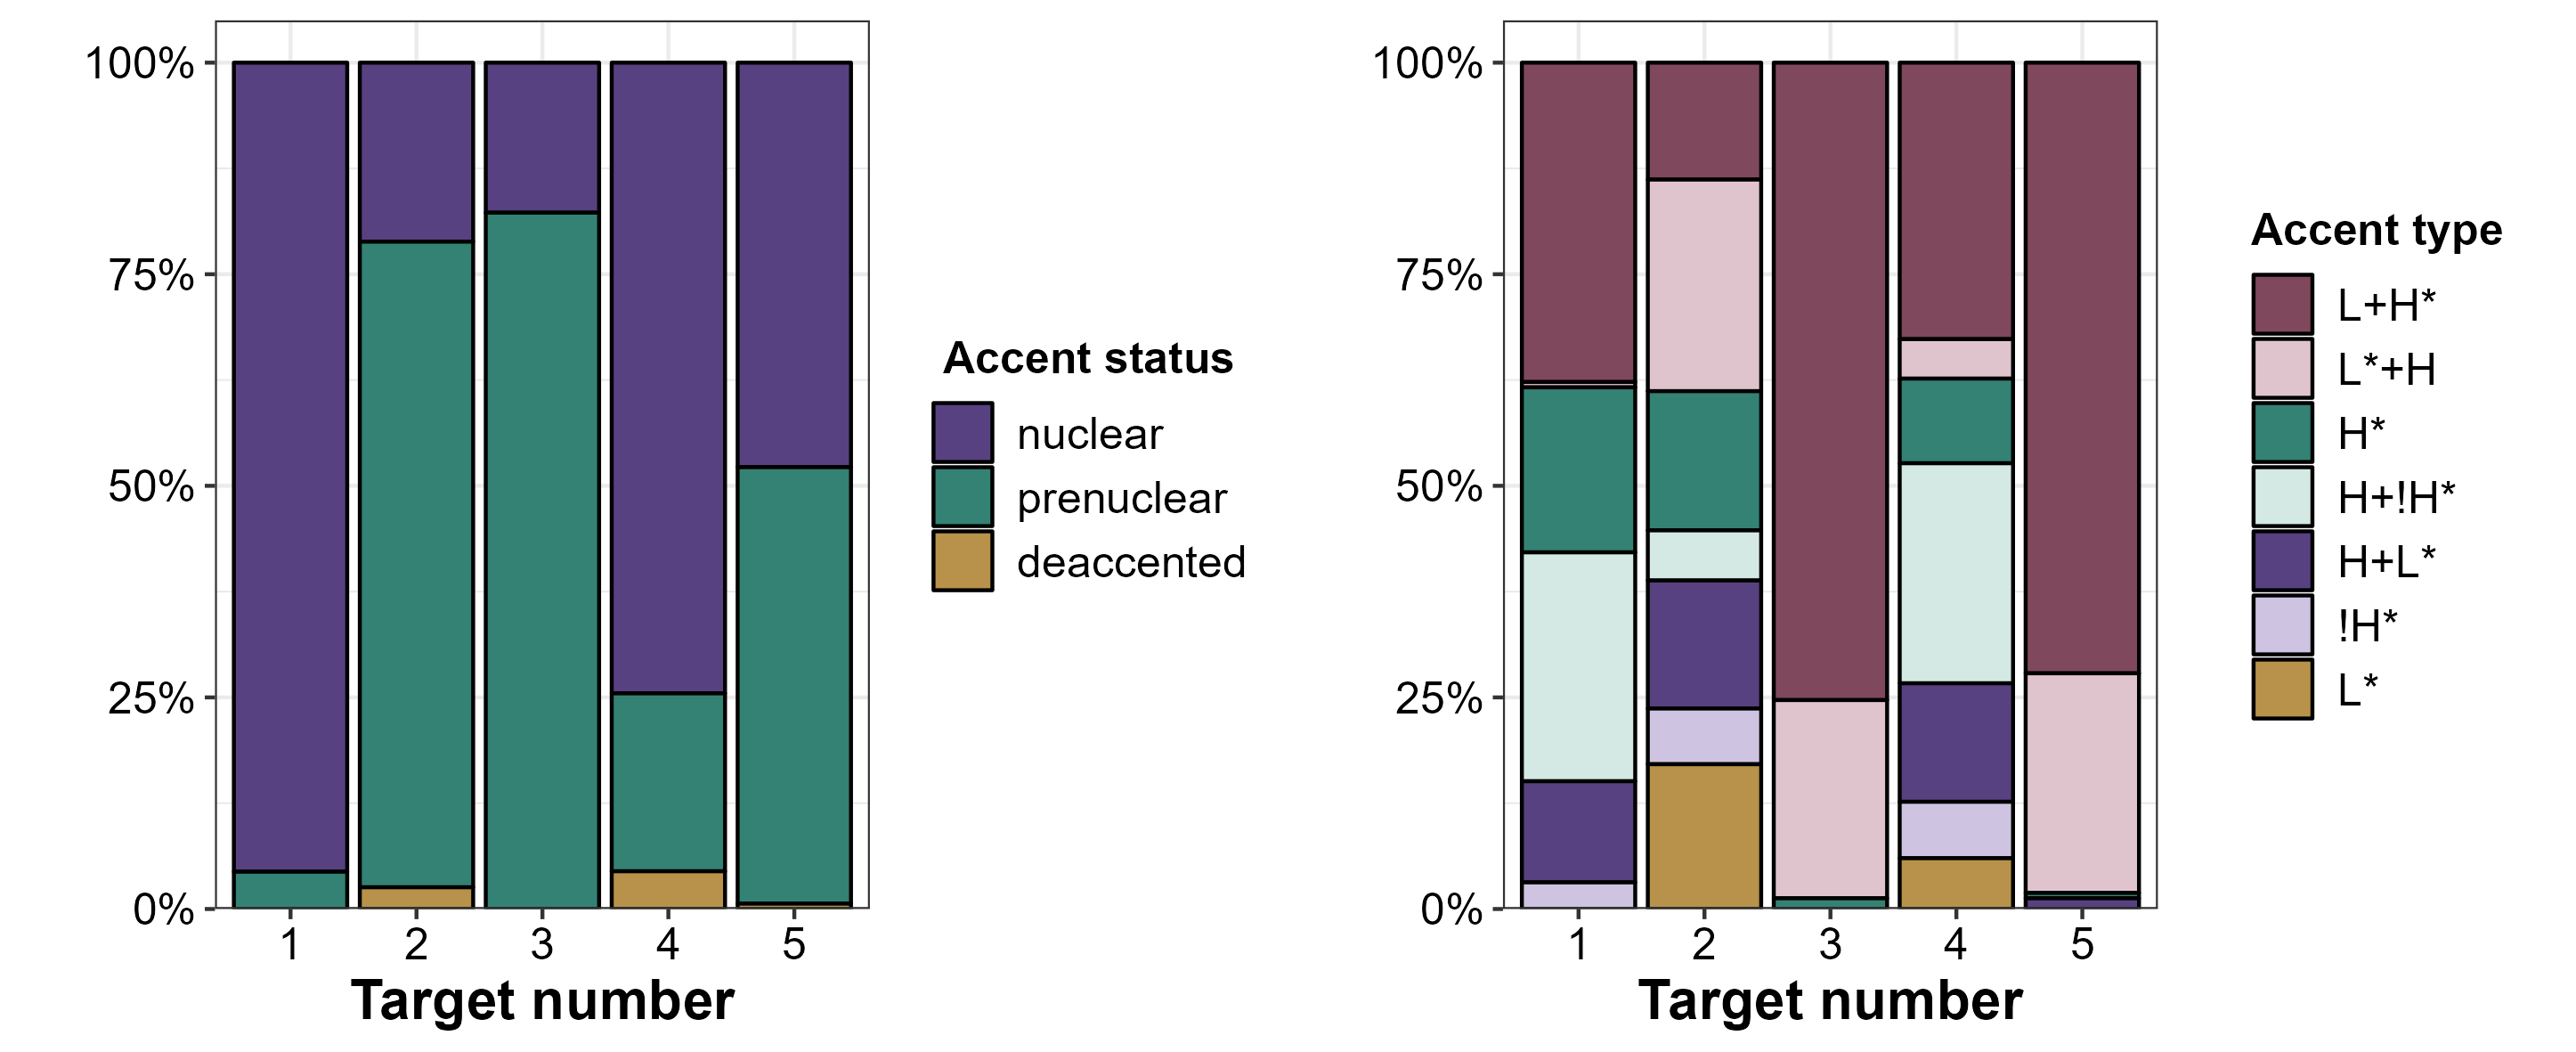
\includegraphics[scale = 0.5]{s2_accent_statustype}
	\caption{Barplots of the distributions of accent status and accent type by target word position.}
	\label{fig:s2_accent_statustype}
\end{figure}

Turning to the continuous prosodic parameters, Figure \ref{fig:s2_cont_parameters} shows the means and standard deviations for each of the eight z-scored prosodic parameters by target word condition. The top panels show the F0-related parameters F0 at CoM, Delta F0, CoG, and synchrony. Average F0 at CoM and Delta F0 values are highest in Targets 3, 5, and 1 and lowest in Target 2, which reflects the accent type distributions reported in the previous paragraph. Similarly, synchrony is on average highest in the initial target words (3 and 5) and is associated with relatively small standard deviations, which is in line with the observation that these words are almost exclusively produced with rising accents. CoG is later aligned in Targets 2 and 3 and earlier in Targets 4 and 5.\footnote{The variability in CoG between the different target word conditions can partially be explained by the different accent types associated with these conditions: Target 4 is produced with more falling accents (characterized by an early CoG) and fewer late rising L*+H accents (characterized by a late CoG) than Target 2 yielding overall earlier CoG alignment in Target 4. However, Target 3 and Target 5 are produced with very similar accent types, yet still differ in CoG alignment. This indicates that CoG as a phonetic parameter is still modified within any category boundaries of different accent types.} The parameters related to timing and intensity on average exhibit the highest values for Target 5, followed by Targets 3 and 1. Target 2 is produced with the lowest intensity and periodic energy mass values, while both Targets 2 and 4 exhibit the shortest average durations.

\begin{figure}
		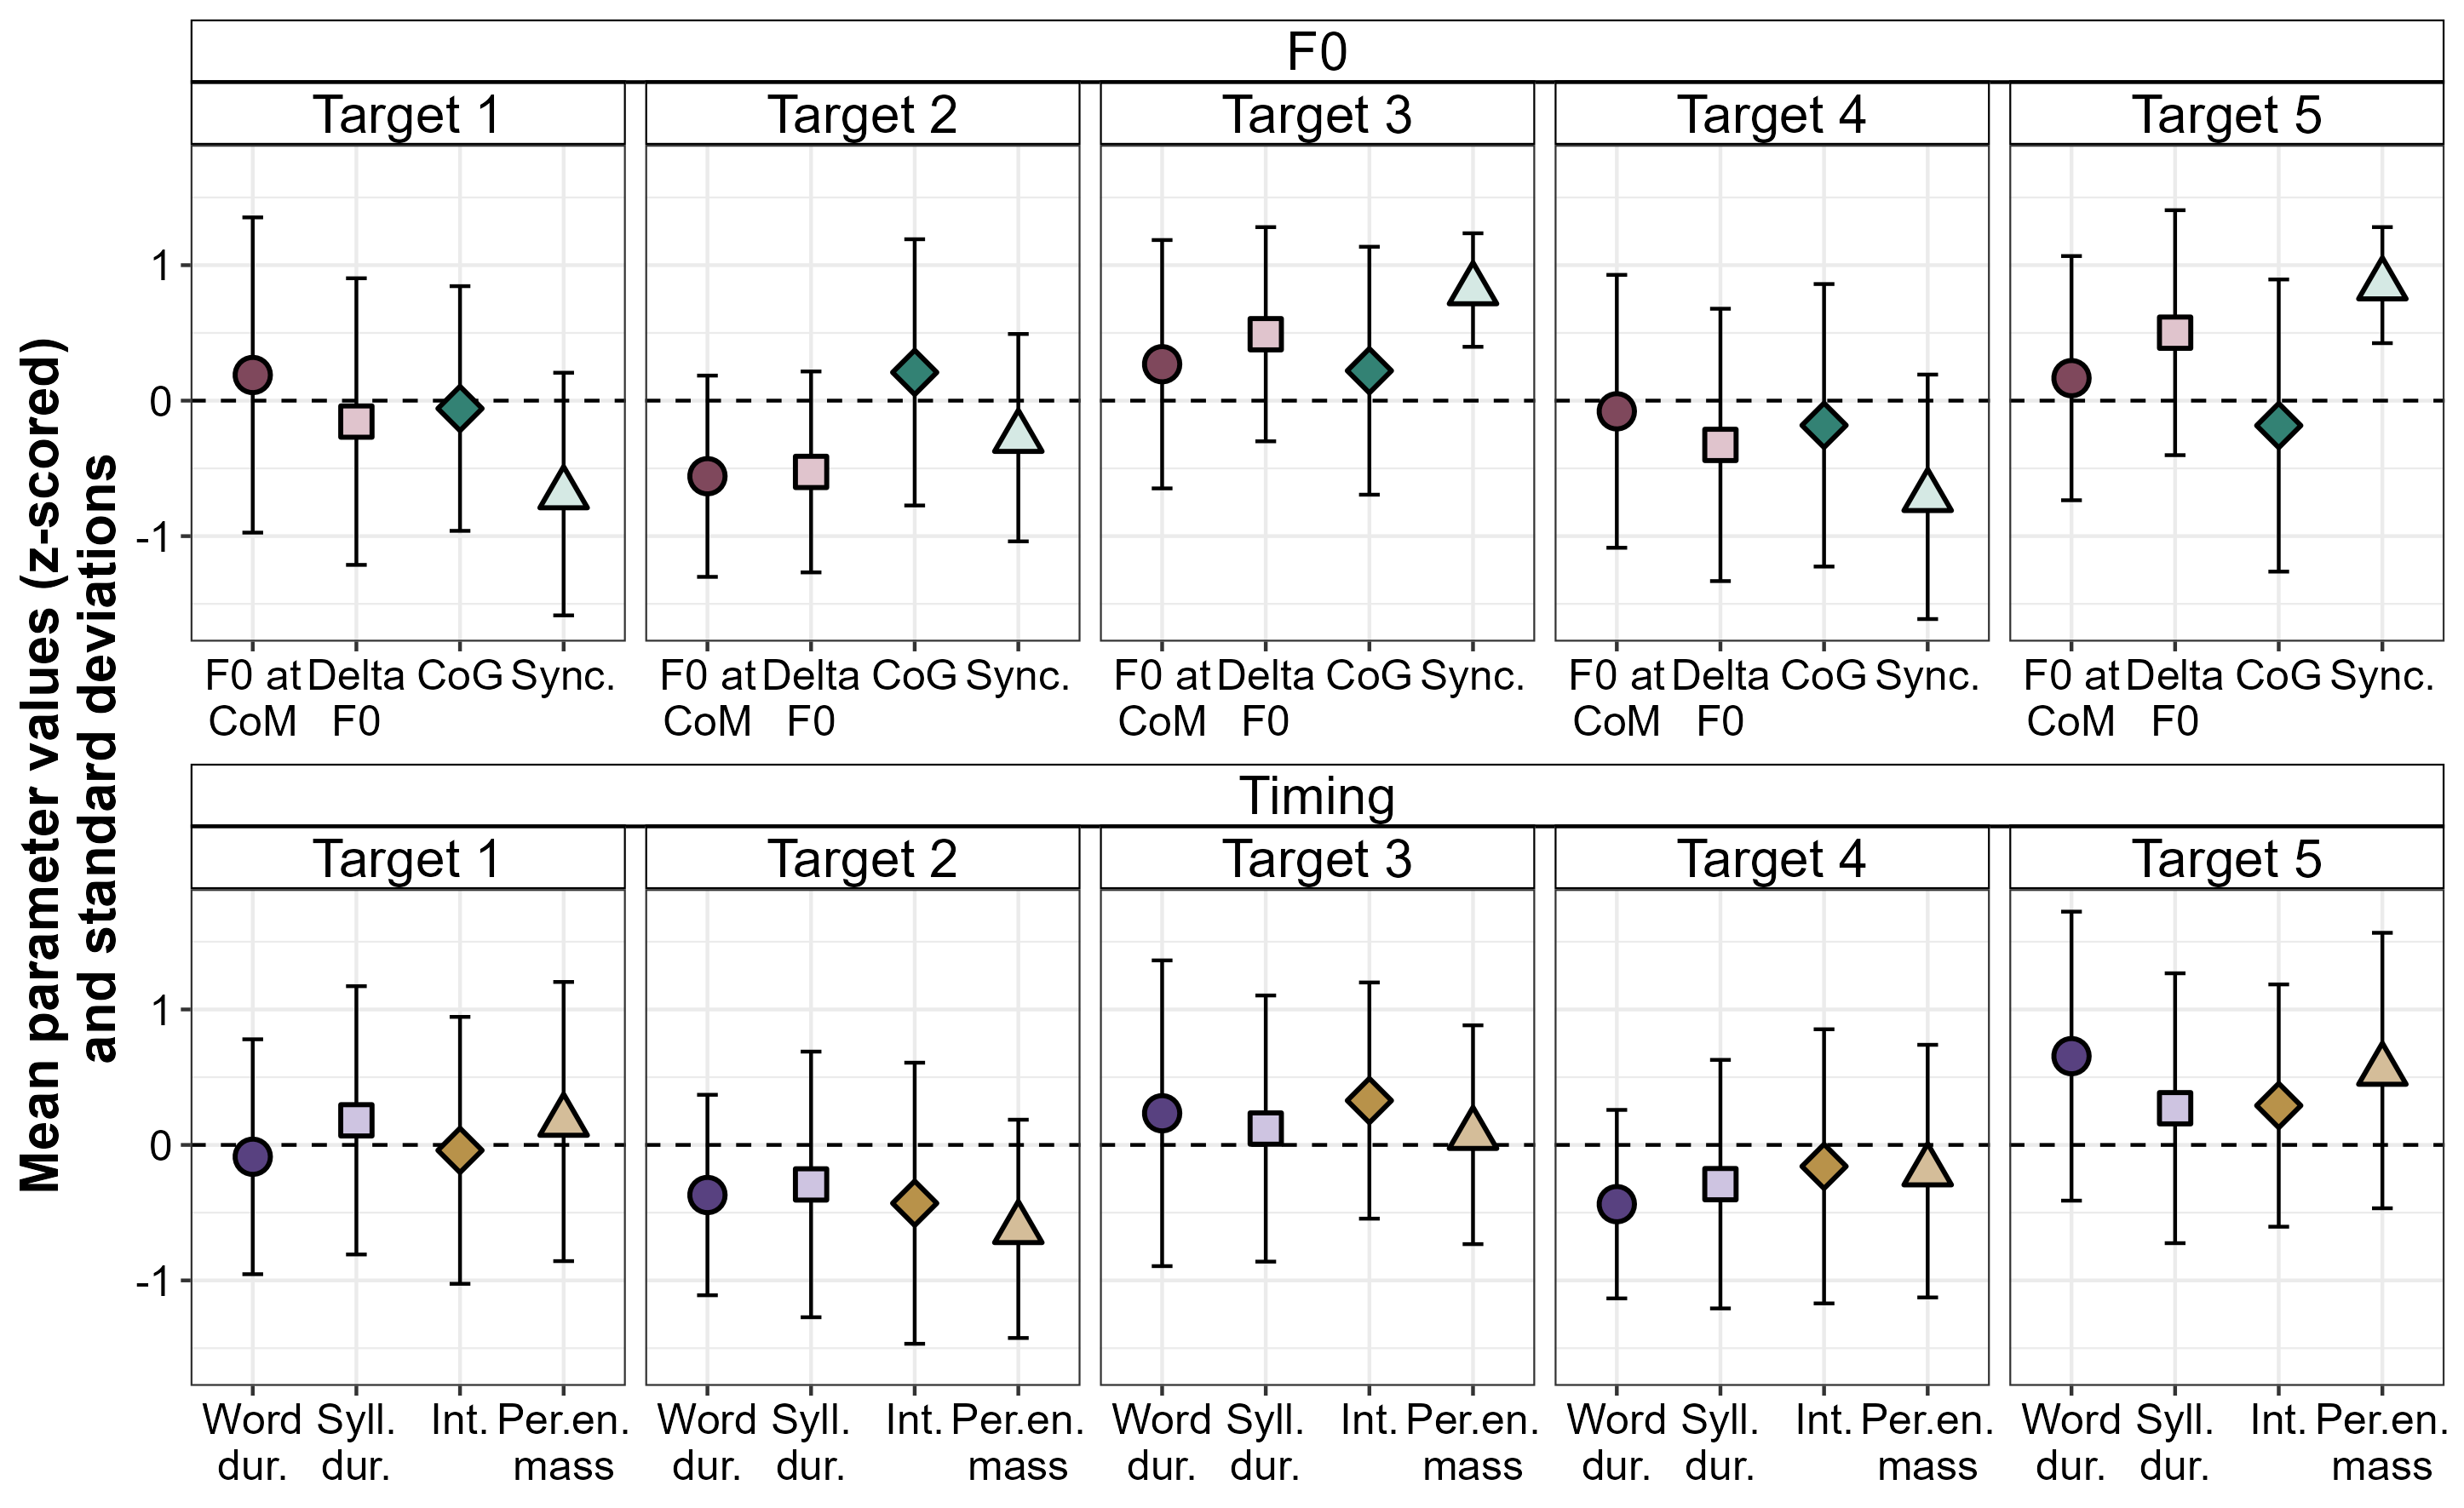
\includegraphics[scale = 0.5]{s2_cont_parameters}
	\caption{Means and standard deviations of all continuous prosodic parameters (z-scored) by target word position. Top panels: Parameters describing the F0 contour. Bottom panels: Parameters related to timing.}
	\label{fig:s2_cont_parameters}
\end{figure}

To disentangle the effects of the manipulated factors on the trends observed in the raw data, we turn to the results of the Bayesian regression models. For lexical givenness, we observe consistent albeit not reliable (following the criteria for reliability specified in Section \ref{sec:Production2 statistics}) effects of accent status and accent type, which are summarized in Table \ref{table:model_parameterscat_lexical_givenness}. Lexically new target words are more likely to be produced with nuclear accents rather than with prenuclear accents or deaccented compared to lexically given target words. They also receive more prominent accent types, although this trend is weaker.

\begin{table}[]
\begin{tabular}{lrrr}
\lsptoprule
\multicolumn{4}{c}{Lexical givenness} \\ \hline
Variable    & $\beta$ & 90\% CrI  & Pr($\beta$\textgreater{}0) \\ \hline
Accent status    & 1.36       & {[}-0.37; 2.91{]}  & 0.91                          \\
Accent type        & 0.38       & {[}-0.31; 1.03{]} & 0.83                          \\
\lspbottomrule
\end{tabular}
\caption{Model parameters describing the effects of lexical givenness on accent status and accent type.}
\label{table:model_parameterscat_lexical_givenness}
\end{table}

Table \ref{table:model_parameters_lexical_givenness} summarizes the model parameters describing the effects of lexical givenness on the continuous prosodic cues. On average, l-new referents are produced with higher values in seven out of the eight prosodic parameters than l-given referents. The strongest, most reliable effects are observed for word duration, syllable duration, and periodic energy mass (Pr($\beta$\textgreater{}0)\textgreater{}0.95), l-new referents being produced with longer duration of the target word and its stressed syllable and higher periodic energy mass in the stressed syllable than l-given referents. There is also strong evidence that l-new referents are produced with higher F0 at CoM and higher intensity in the stressed syllable relative to l-given referents. Furthermore, l-new referents appear to exhibit higher Delta F0 and a later CoG, however, evidence to support these tendencies is much weaker. Finally, synchrony does not appear to vary systematically between l-new and l-given referents with a $\beta$ estimate close to 0.

\begin{table}[]
\begin{tabular}{lrrr}
\lsptoprule
\multicolumn{4}{c}{Lexical givenness} \\ \hline
Variable    & $\beta$ & 90\% CrI  & Pr($\beta$\textgreater{}0) \\ \hline
F0 at CoM    & 0.19       & {[}0.00; 0.38{]}  & 0.95                          \\
Delta F0    & 0.09       & {[}-0.15; 0.34{]}  & 0.75                          \\
Center of Gravity            & 0.09       & {[}-0.14; 0.31{]}  & 0.76                          \\
Synchrony            & -0.02       & {[}-0.28; 0.25{]}  & 0.45                          \\
Word duration            & 0.31       & {[}0.09; 0.53{]}  & 0.99                          \\
Syllable duration & 0.43       & {[}0.20; 0.65{]}  & 1.00                             \\
Intensity             & 0.13       & {[}0.00; 0.26{]} & 0.95                          \\
Periodic energy mass         & 0.36       & {[}0.18; 0.52{]} & 1.00                          \\
\lspbottomrule
\end{tabular}
\caption{Model parameters describing the effects of lexical givenness on the continuous prosodic parameters.}
\label{table:model_parameters_lexical_givenness}
\end{table}

Referential givenness influences accent status in the expected direction, i.e., r-new target words are more likely produced with nuclear accents than r-given target words, although this effect is not reliable (see Table \ref{table:model_parameterscat_referential_givenness}). Accent type does not appear to systematically encode referential givenness.

\begin{table}[]
\begin{tabular}{lrrr}
\lsptoprule
\multicolumn{4}{c}{Referential givenness} \\ \hline
Variable    & $\beta$ & 90\% CrI  & Pr($\beta$\textgreater{}0) \\ \hline
Accent status    & 1.33       & {[}-0.25; 2.78{]}  & 0.92                         \\
Accent type        & 0.13       & {[}-0.71; 0.92{]} & 0.61                          \\
\lspbottomrule
\end{tabular}
\caption{Model parameters describing the effects of referential givenness on accent status and accent type.}
\label{table:model_parameterscat_referential_givenness}
\end{table}

Table \ref{table:model_parameters_referential_givenness} summarizes the model parameters describing the effects of referential givenness on the continuous prosodic cues. R-new referents are reliably marked by a higher F0 at CoM, higher intensity, and higher periodic energy mass of the stressed syllable (Pr($\beta$\textgreater{}0)\textgreater{}0.95) compared to r-given referents. In addition, there is some evidence for a higher Delta F0 in r-new referents. Contrary to expectations, there is reliable evidence that r-new referents are produced with an earlier CoG and lower synchrony than r-given referents (Pr($\beta$\textgreater{}0)\textless{}0.05), indicating an earlier alignment of the F0 peak. While it appears that word duration tends to be longer in r-given referents, syllable duration does not encode referential givenness with a posterior distribution centered around 0.

\begin{table}[]
\begin{tabular}{lrrr}
\lsptoprule
\multicolumn{4}{c}{Referential givenness} \\ \hline
Variable    & $\beta$ & 90\% CrI  & Pr($\beta$\textgreater{}0) \\ \hline
F0 at CoM    & 0.45       & {[}0.20; 0.69{]}  & 1.00                          \\
Delta F0    & 0.18       & {[}-0.10; 0.46{]}  & 0.86                          \\
Center of Gravity            & -0.37       & {[}-0.62; -0.12{]}  & 0.01                          \\
Synchrony            & -0.43       & {[}-0.81; -0.05{]}  & 0.03                          \\
Word duration            & -0.06       & {[}-0.19; 0.07{]}  & 0.21                          \\
Syllable duration & 0.00       & {[}-0.23; 0.22{]}  & 0.50                             \\
Intensity             & 0.26       & {[}0.12; 0.39{]} & 1.00                          \\
Periodic energy mass         & 0.41       & {[}0.23; 0.59{]} & 1.00                          \\
\lspbottomrule
\end{tabular}
\caption{Model parameters describing the effects of referential givenness on the continuous prosodic parameters.}
\label{table:model_parameters_referential_givenness}
\end{table}

For grammatical role, there is a reliable effect on accent status in that objects are more likely to occupy stronger metrical positions than subjects (see Table \ref{table:model_parameterscat_gramm_role}). However, the effect of grammatical role on accent type is reversed, with subjects receiving more prominent accent types than objects, but also somewhat weaker. 

\begin{table}[]
\begin{tabular}{lrrr}
\lsptoprule
\multicolumn{4}{c}{Grammatical role} \\ \hline
Variable    & $\beta$ & 90\% CrI  & Pr($\beta$\textgreater{}0) \\ \hline
Accent status    & 1.33       & {[}0.60; 2.03{]}  & 1.00                          \\
Accent type        & -0.29       & {[}-0.83; 0.25{]} & 0.19                          \\
\lspbottomrule
\end{tabular}
\caption{Model parameters describing the effects of grammatical role on accent status and accent type.}
\label{table:model_parameterscat_gramm_role}
\end{table}

In contrast to lexical and referential givenness, the marking of grammatical role is more subtle in terms of continuous prosodic parameters (see Table \ref{table:model_parameters_gramm_role}). Reliable evidence from the models suggests that objects are produced with an earlier CoG compared to subjects (Pr($\beta$\textgreater{}0)\textless{}0.05). There is also relatively strong evidence that objects are produced with longer syllable duration and higher periodic energy mass than subjects. Weaker evidence suggests that Delta F0, synchrony, and word duration values are higher, while F0 at CoM and intensity of the stressed syllable are lower in objects than in subjects.  

\begin{table}[]
\begin{tabular}{lrrr}
\lsptoprule
\multicolumn{4}{c}{Grammatical role} \\ \hline
Variable    & $\beta$ & 90\% CrI  & Pr($\beta$\textgreater{}0) \\ \hline
F0 at CoM    & -0.09       & {[}-0.22; 0.03{]}  & 0.11                          \\
Delta F0    & 0.04       & {[}-0.11; 0.18{]}  & 0.67                          \\
Center of Gravity            & -0.33       & {[}-0.60; -0.06{]}  & 0.03                          \\
Synchrony            & 0.05       & {[}-0.08; 0.17{]}  & 0.73                          \\
Word duration            & 0.11       & {[}-0.09; 0.31{]}  & 0.82                          \\
Syllable duration & 0.16       & {[}0.00; 0.33{]}  & 0.94                             \\
Intensity             & -0.04       & {[}-0.17; 0.09{]} & 0.30                          \\
Periodic energy mass         & 0.48       & {[}-0.03; 0.95{]} & 0.94                          \\
\lspbottomrule
\end{tabular}
\caption{Model parameters describing the effects of grammatical role on the continuous prosodic parameters.}
\label{table:model_parameters_gramm_role}
\end{table}

Finally, the results for the effect of sentence position on prosody production are very clear, albeit unexpected under the original expectation that words in medial position should be produced with more prosodic prominence than words in initial position. Instead, the initial position is more prominent in terms of both metrical structure (although this effect is not reliable) and accent type choice (see Table \ref{table:model_parameterscat_position}).

\begin{table}[]
\begin{tabular}{lrrr}
\lsptoprule
\multicolumn{4}{c}{Sentence position} \\ \hline
Variable    & $\beta$ & 90\% CrI  & Pr($\beta$\textgreater{}0) \\ \hline
Accent status    & -0.74       & {[}-1.83; 0.44{]}  & 0.14                          \\
Accent type        & -2.80       & {[}-3.78; -1.73{]} & 0.00                          \\
\lspbottomrule
\end{tabular}
\caption{Model parameters describing the effects of sentence position on accent status and accent type.}
\label{table:model_parameterscat_position}
\end{table}

A similar picture emerges for the continuous prosodic parameters. There is reliable evidence that all but one parameter are produced with higher values in an initial than in a medial target word (all Pr($\beta$\textgreater{}0)\textless{}0.05, see Table \ref{table:model_parameters_position}). That is, initial target words are produced with a higher F0 at CoM, higher Delta F0, higher synchrony, longer word and syllable duration, higher intensity, and higher periodic energy mass in the stressed syllable. The one exception is CoG, where there is quite strong evidence that words in medial position are produced with a later CoG than words in initial position. Sentence position thus appears to be the most important factor in modulating prosodic prominence.

\begin{table}[]
\begin{tabular}{lrrr}
\lsptoprule
\multicolumn{4}{c}{Sentence position} \\ \hline
Variable    & $\beta$ & 90\% CrI  & Pr($\beta$\textgreater{}0) \\ \hline
F0 at CoM    & -0.69       & {[}-1.00; -0.36{]}  & 0.00                          \\
Delta F0    & -0.96       & {[}-1.28; -0.63{]}  & 0.00                          \\
Center of Gravity            & 0.35       & {[}-0.04; 0.72{]}  & 0.94                          \\
Synchrony            & -1.10       & {[}-1.38; -0.82{]}  & 0.00                          \\
Word duration            & -0.51       & {[}-0.73; -0.30{]}  & 0.00                          \\
Syllable duration & -0.52       & {[}-0.83; -0.20{]}  & 0.01                             \\
Intensity             & -0.71       & {[}-0.90; -0.52{]} & 0.00                          \\
Periodic energy mass         & -1.23       & {[}-1.62; -0.80{]} & 0.00                          \\
\lspbottomrule
\end{tabular}
\caption{Model parameters describing the effects of sentence position on the continuous prosodic parameters.}
\label{table:model_parameters_position}
\end{table}

\subsection{Individual strategies}

After establishing a baseline of the overall effects across speakers, this section explores individual differences and similarities in the prosodic encoding of lexical and referential givenness, grammatical role, and sentence position. As in the previous study (see Chapter \ref{ch:Production I}), we first take a descriptive approach to individual variability. Figure \ref{fig:s2_accent_status_byspeaker} illustrates the distribution of accent status across the five target word conditions for each speaker. Most obviously, only five out of 20 speakers use deaccentuation at all. A similarity is that for all speakers except one (s16), Target 1 is the most likely to be produced with a nuclear accent, i.e., the most prominent, and in fact, 16 speakers produce Target 1 exclusively with a nuclear accent. For most speakers (n = 16), Target 4 is the second most likely to receive a nuclear accent or equally as likely as Target 1. There are three speakers who produce Target 5 more prominently than Target 4, namely, s05, s09, and s20. Looking at only the medial target words (1, 2, and 4), Target 2 is consistently the least prominent of the three for every speaker, as it is produced with at most 50\% nuclear accents (s03, s13) but more often with exclusively prenuclear accents (s07, s09, s11, s17). There is more variability with regard to the initial target words (3 and 5). Some speakers produce only prenuclear accents in both positions (s04, s07, s14, s16) but one speaker (s09) produces only nuclear accents on Target 5. In most speakers (n = 14), Target 5 is more likely to receive a nuclear accent than Target 3. 

\begin{figure}
		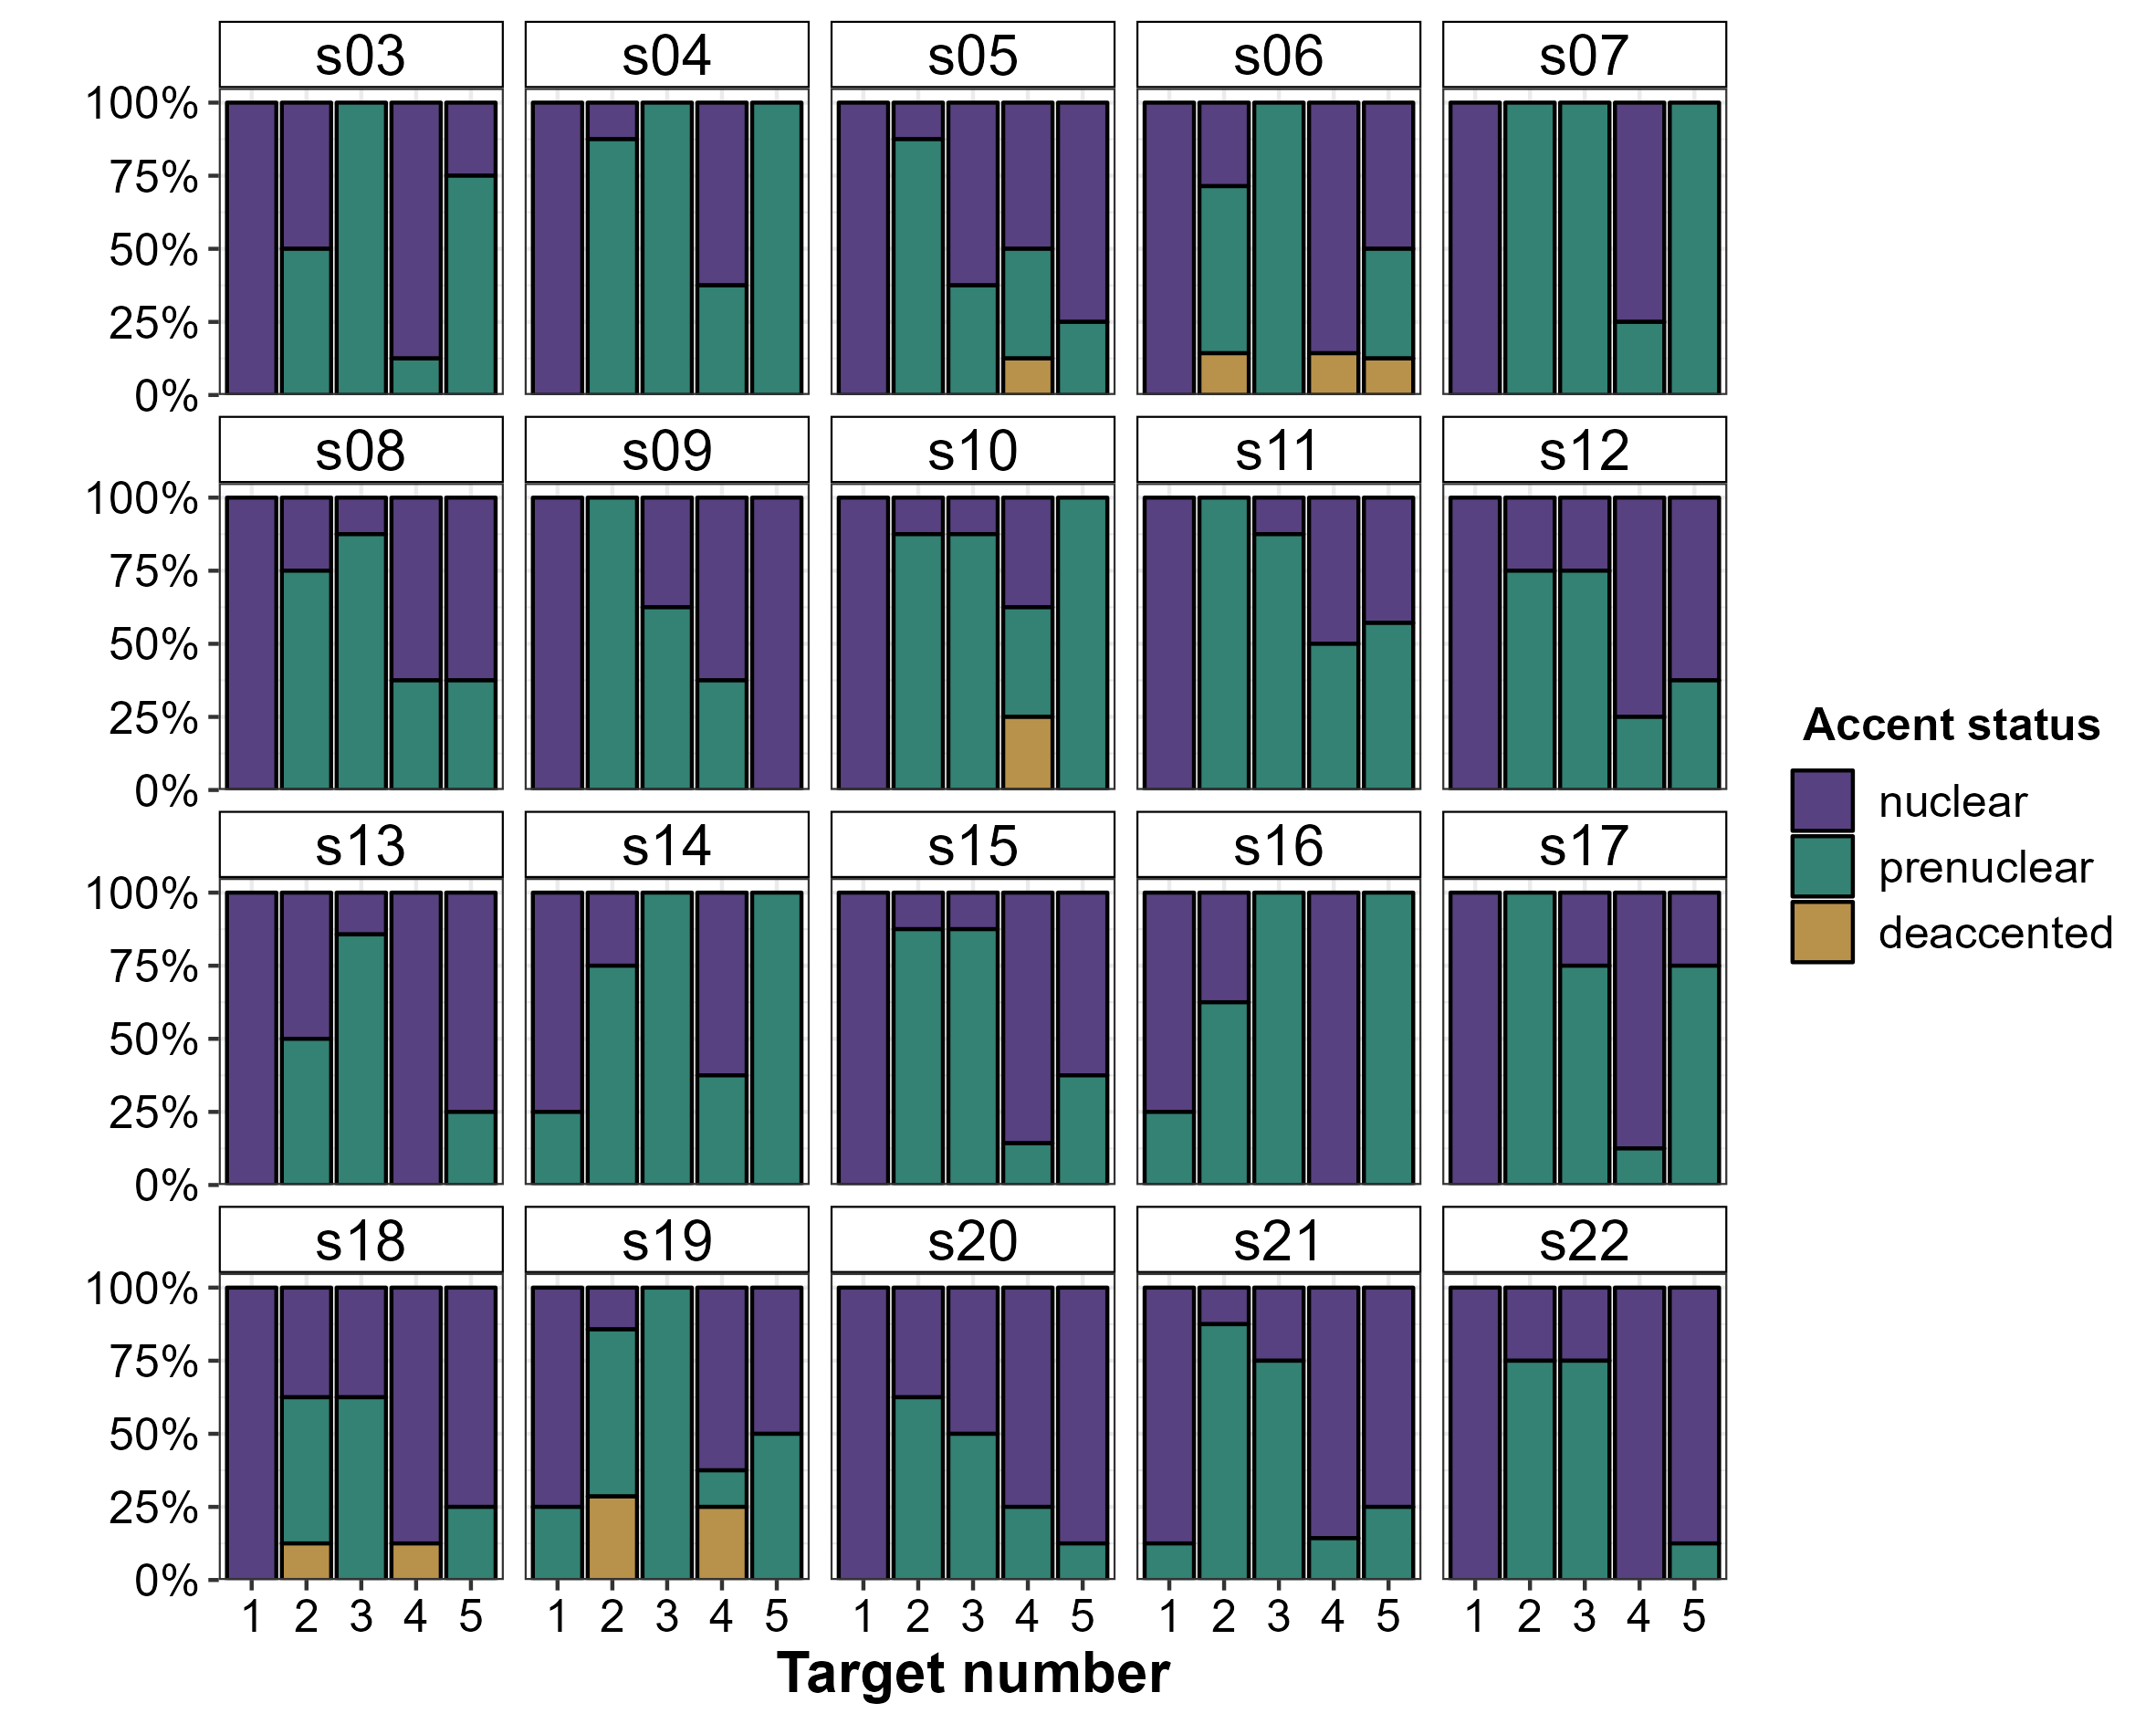
\includegraphics[width=\textwidth]{s2_accent_status_byspeaker}
	\caption{Distributions of accent status across target word positions per speaker.}
	\label{fig:s2_accent_status_byspeaker}
\end{figure}

Next, we look at the usage of pitch accent types across the target word conditions (see Figure \ref{fig:s2_accent_type_byspeaker}). There is generally more variability in terms of accent types used in the medial target words (1, 2, and 4) than the initial ones (3 and 5) and initial target words are produced consistently with more prominent accent types across speakers, which is in line with the averaged result in Section \ref{sec:Production2 overall results} above. In fact, ten speakers produce only L*+H and L+H* accents on initial target words and another six speakers produce exclusively L+H* accents on Targets 3 and 5. In contrast to the prominence ranking observed for Targets 3 and 5 in terms of accent status, the accent type distributions do not yield such clear results. Specifically, there are only four speakers (s05, s12, s13, and s17) who use more prominent accent types on Target 5 than Target 3, but seven speakers (s04, s06, s09, s14, s15, s20, s22) who use more prominent accent types on Target 3. In the medial target words (1, 2, and 4), speakers typically use between two and five different accent types per condition. Due to this diversity, it is much harder to detect systematic patterns by visually inspecting the plots. Nevertheless, half of the speakers (s06, s07, s08, s11, s12, s13, s15, s19, s20, and s21) use more L+H* (i.e., the most prominent accent type) in  Target 1 than in Targets 2 and 4, which is in the anticipated direction. In addition, Target 2, which was expected to be the least prominent of the medial target words, is realized with a larger proportion of the least prominent L* accent than Targets 1 and 4 by eight speakers (s04, s07, s09, s12, s13, s17, s19, s21). However, the prominence ranking between  Targets 1 and 4 in terms of accent type is not at all clear. Focusing on just the proportions of L+H*, only six speakers exhibit the expected ranking of 1 > 4 > 2 (s07, s08, s15, s19, s20, s21). In contrast, eight speakers produce their highest proportions of L+H* (in medial target words) in Target 2 (s05, s17) or Target 4 (s04, s09, s10, s16, s18, s22). This reflects the inconclusive overall results concerning accent type presented in Section \ref{sec:Production2 overall results}, especially regarding the effects of referential givenness. 

\begin{figure}
		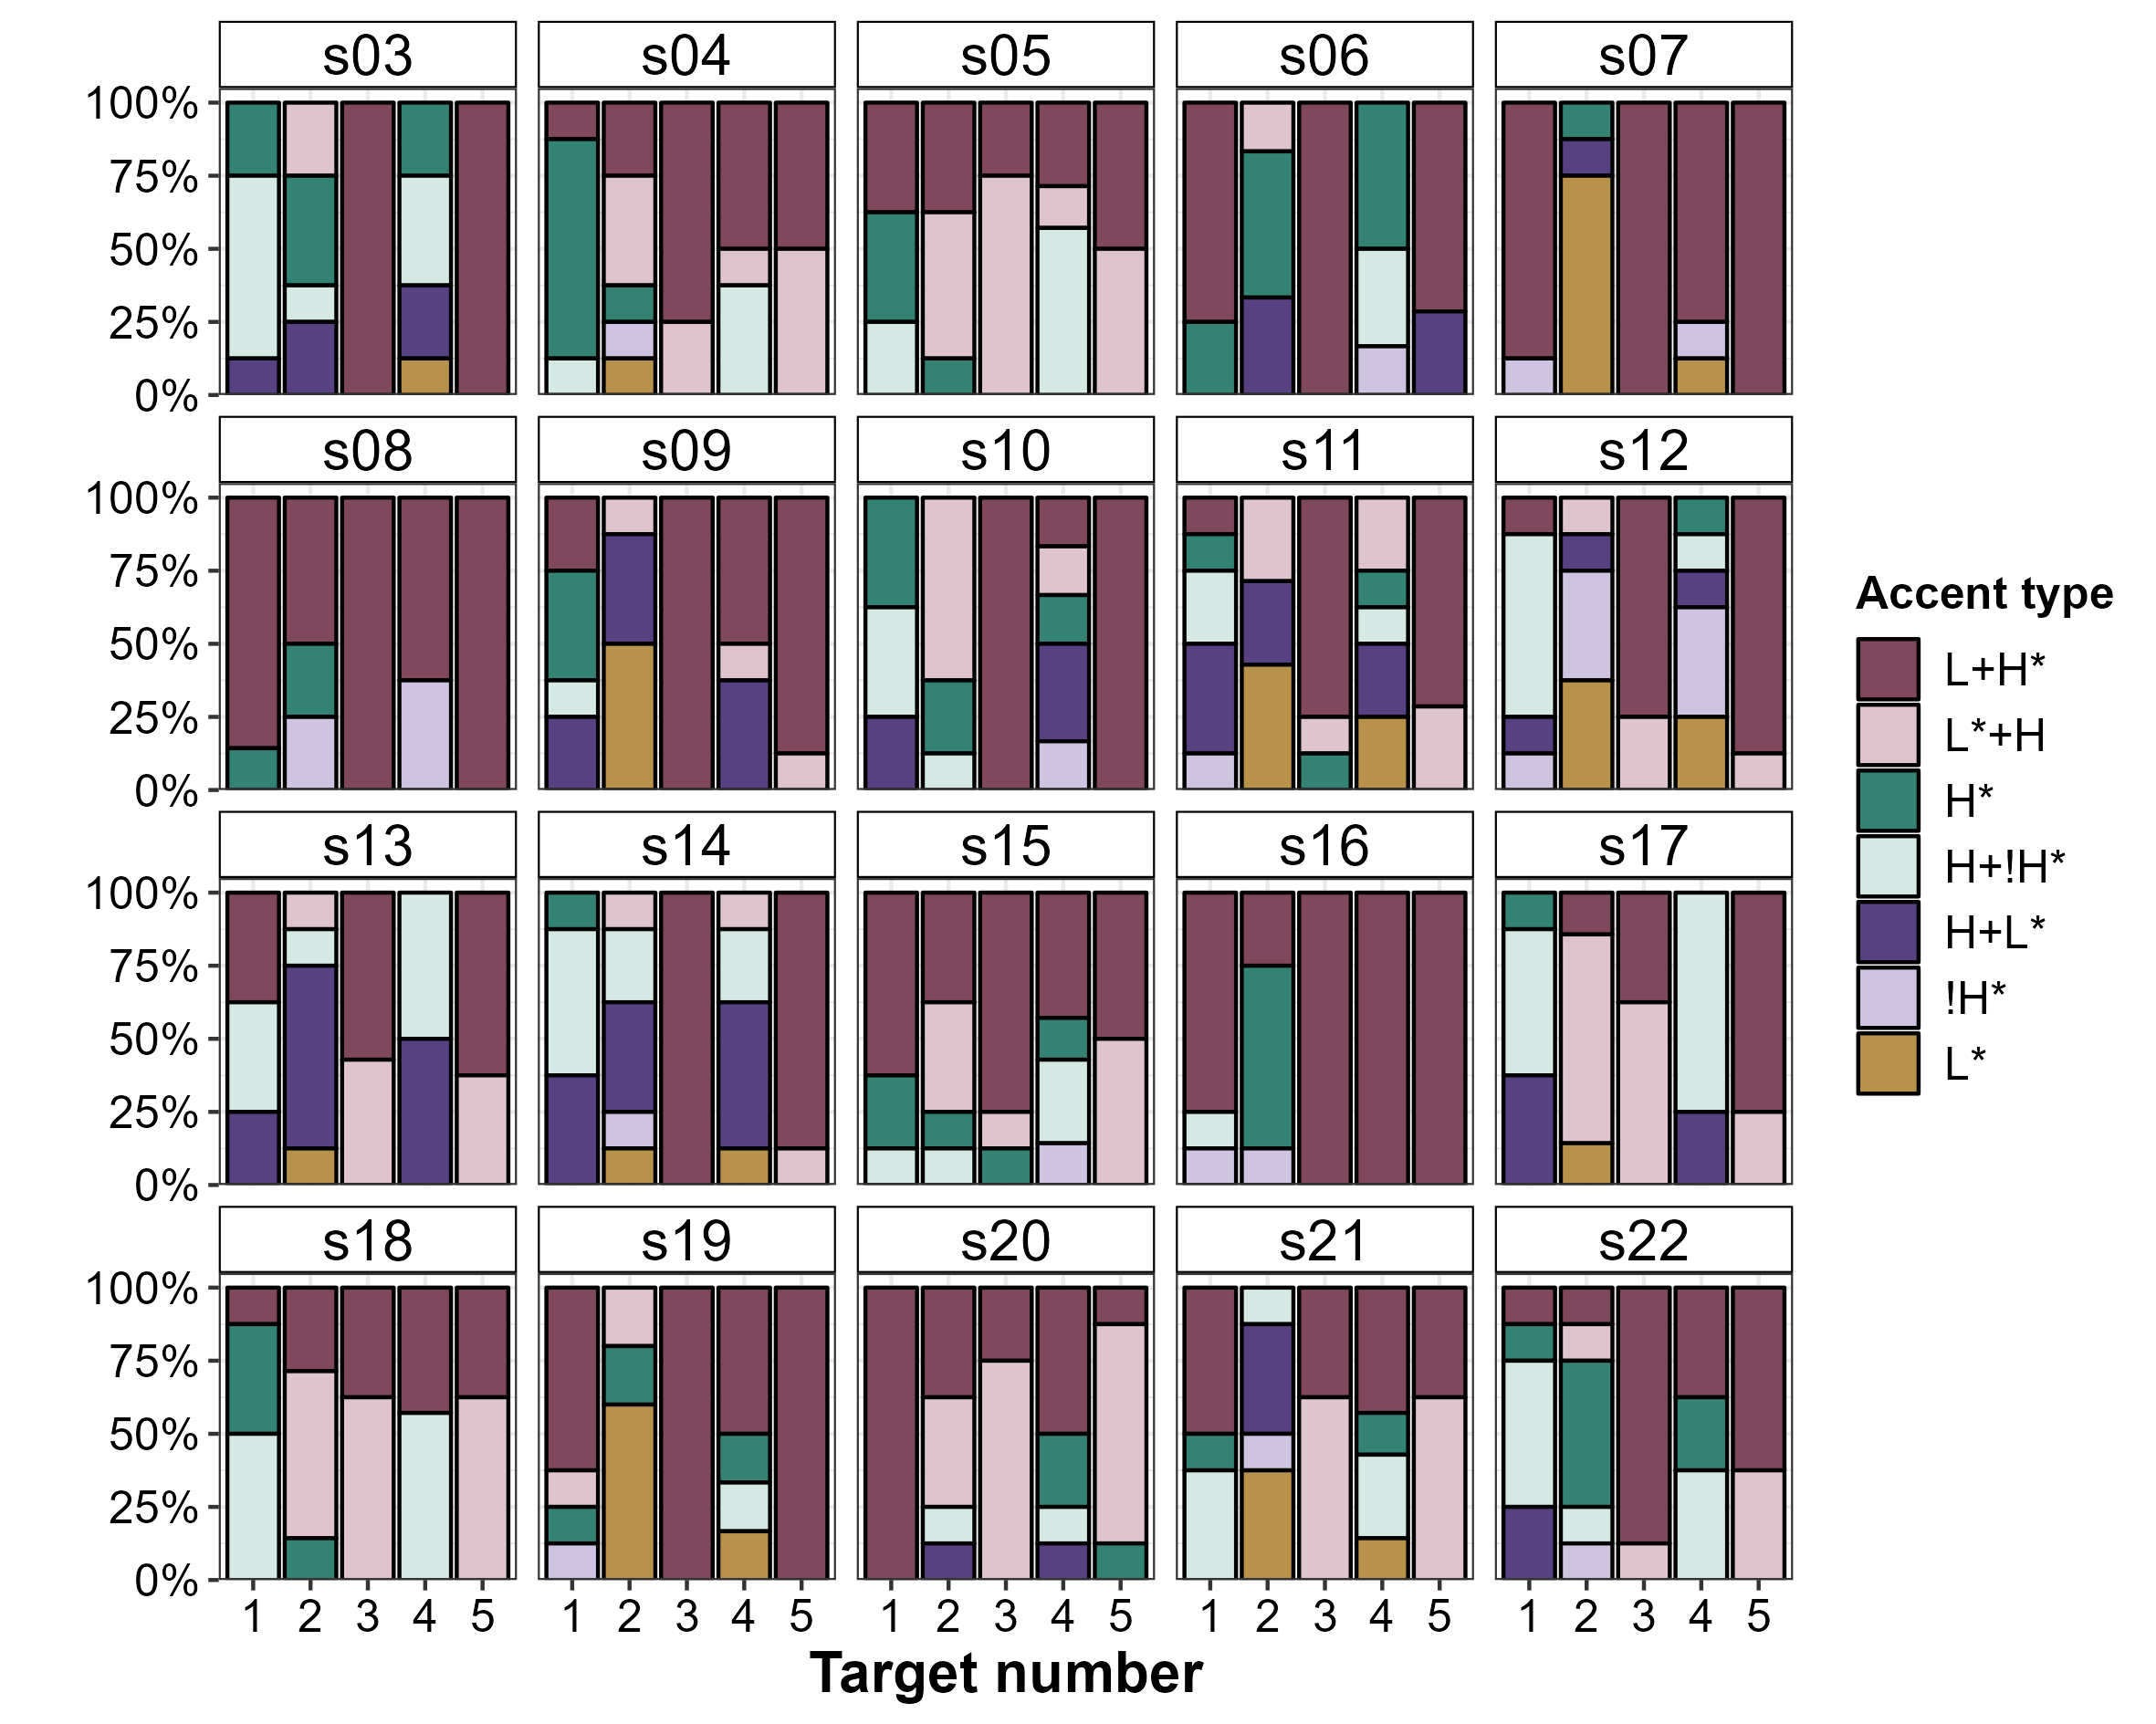
\includegraphics[width=\textwidth]{s2_accent_type_byspeaker}
	\caption{Distributions of pitch accent types across target word positions per speaker.}
	\label{fig:s2_accent_type_byspeaker}
\end{figure}

To more systematically analyze the inter-speaker variability observed in the encoding of the individual semantic-pragmatic and syntactic factors via accent type and accent status, we return to the output of the regression models presented in the previous section. Figure \ref{fig:s2_accentstatus_effects} presents the estimated effect of each of the four factors on accent status per speaker, i.e., the random slope estimates from the accent status model. For lexical givenness, most speakers (18 out of 20) likely produce new target words in such a way that they occupy stronger metrical positions than given words as indicated by the positive mean posterior estimates in Figure \ref{fig:s2_accentstatus_effects} (upper left panel). However, for quite a few speakers, the 90\% CrIs considerably overlap with zero, indicating there is a probability that they exhibit no effect. This is different for referential givenness (Figure \ref{fig:s2_accentstatus_effects}, upper right panel), where 15 speakers clearly show the expected effect of referential givenness on accent status with fully positive 90\% CrIs of the posterior estimates. What is more, mean posterior estimates are positive for all speakers. The number of speakers showing a clearly positive effect of grammatical role on accent status is slightly lower, with 12 speakers producing objects in metrically stronger positions than subjects (Figure \ref{fig:s2_accentstatus_effects}, bottom left panel). Nevertheless, mean estimates are positive throughout all speakers. Finally, for sentence position, seven speakers reliably produce more nuclear accents in the initial position than the medial one (Figure \ref{fig:s2_accentstatus_effects}, bottom right panel). There are also some speakers potentially showing the opposite effect, more prominent accent status in medial target words, although these speakers' 90\% CrIs include zero, indicating the possibility of a null effect. 

\begin{figure}[t]	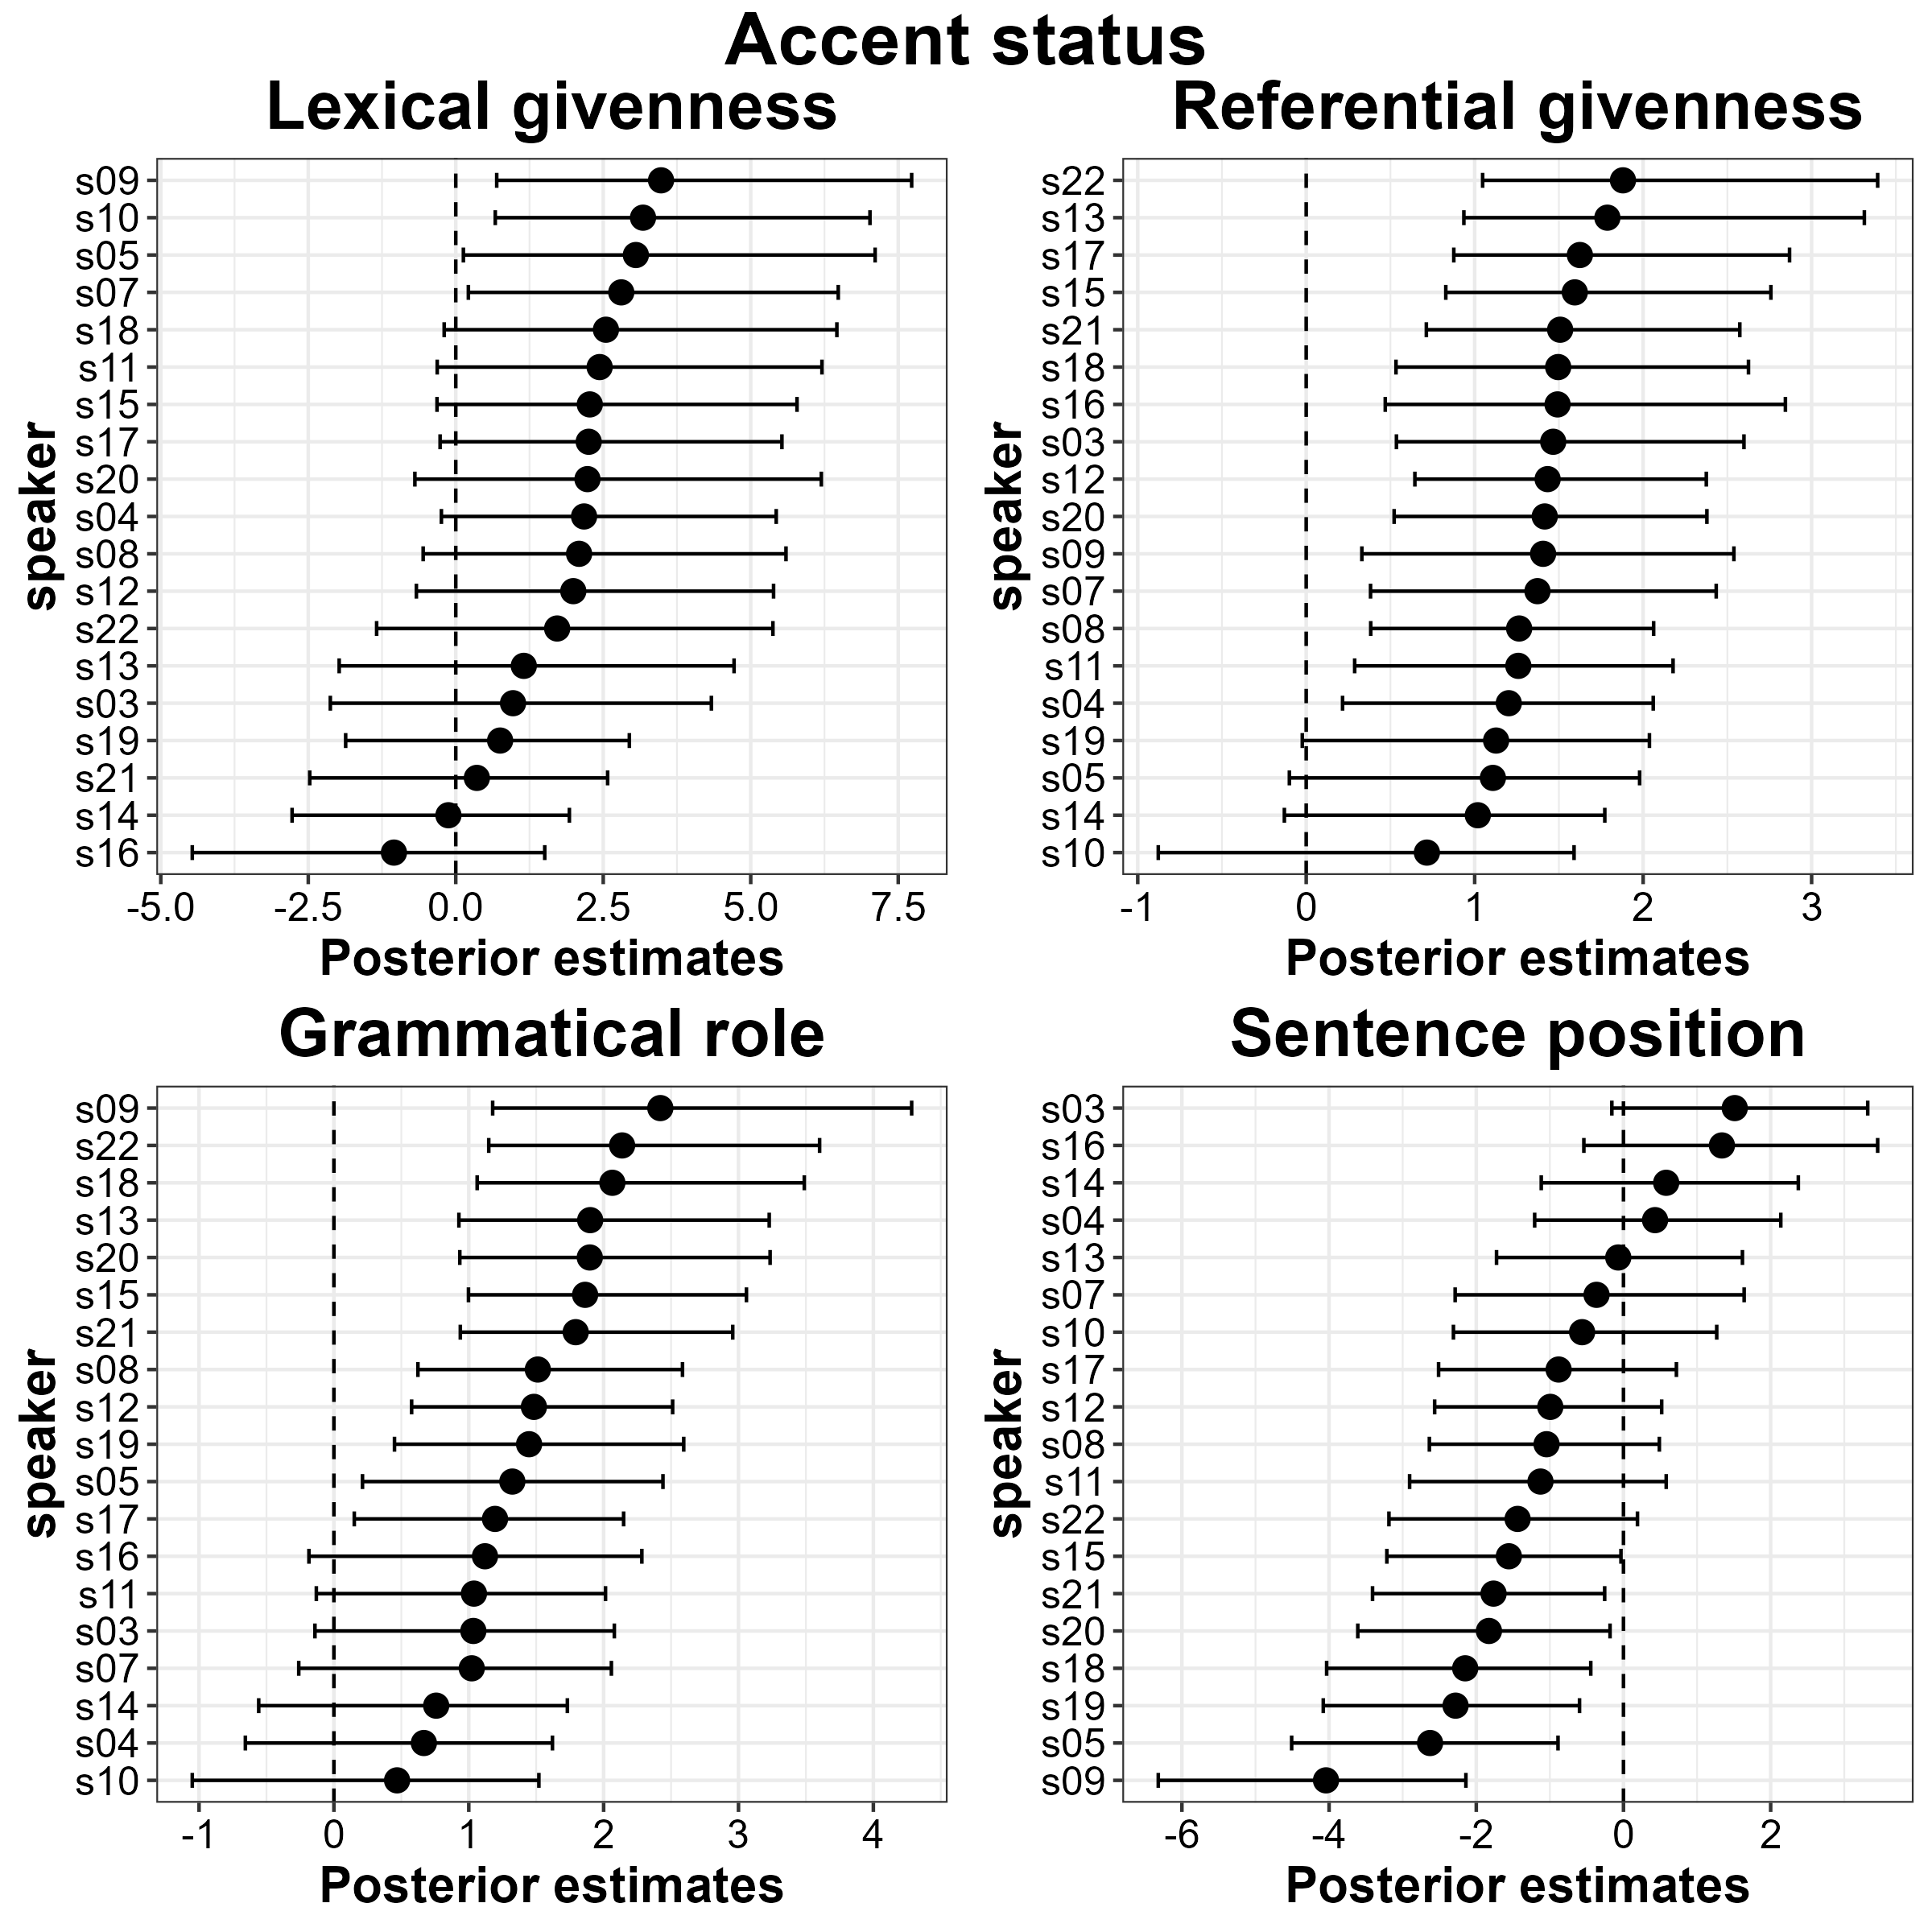
\includegraphics[scale = 0.5]{s2_accentstatus_effects}
	\caption{Means and 90\% CrIs for the effects of lexical and referential givenness, grammatical role, and sentence position on accent status.}
	\label{fig:s2_accentstatus_effects}
\end{figure}

Moving on to the second categorical parameter, accent type, there are two speakers who reliably use more prominent accent types to mark lexical newness (see Figure \ref{fig:s2_accenttype_effects}, upper left panel). In addition, six speakers seem to show relatively strong effects of lexical givenness on accent type. However, the remaining speakers do not seem to make use of this parameter to a reliable extent, with mean posterior estimates close to zero. For referential givenness, there is considerable individual variability in the use of accent type (see Figure \ref{fig:s2_accenttype_effects}, upper right panel). While half of the speakers show a reliable or relatively strong positive effect (i.e., producing more prominent accent types on referentially new entities), three speakers exhibit a reliable effect in the opposite direction, marking referentially given entities with more prominent accent types. Note that the speakers exhibiting the strongest effects of lexical and referential givenness on accent type are not identical to the speakers showing the strongest effects on accent status, i.e. speakers who use accent status to encode either dimension of givenness do not simultaneously make use of accent type to the same end. In fact, speaker s17, who shows one of the strongest positive effects of referential givenness on accent status, produces the strongest negative effect of referential givenness on accent type.

In contrast to the results for referential givenness, there is little variability in the encoding of grammatical role via accent type across speakers (see Figure \ref{fig:s2_accenttype_effects}, bottom left panel). If anything, all speakers have a weak tendency to produce more prominent accent types on subjects than on objects. Finally, there is also little variability in the encoding of sentence position (see Figure \ref{fig:s2_accenttype_effects}, bottom right panel). All speakers exhibit negative effects, i.e., the initial position is associated with more prominent accent types than the medial position. This effect is reliable for 14 speakers. 

\begin{figure}
		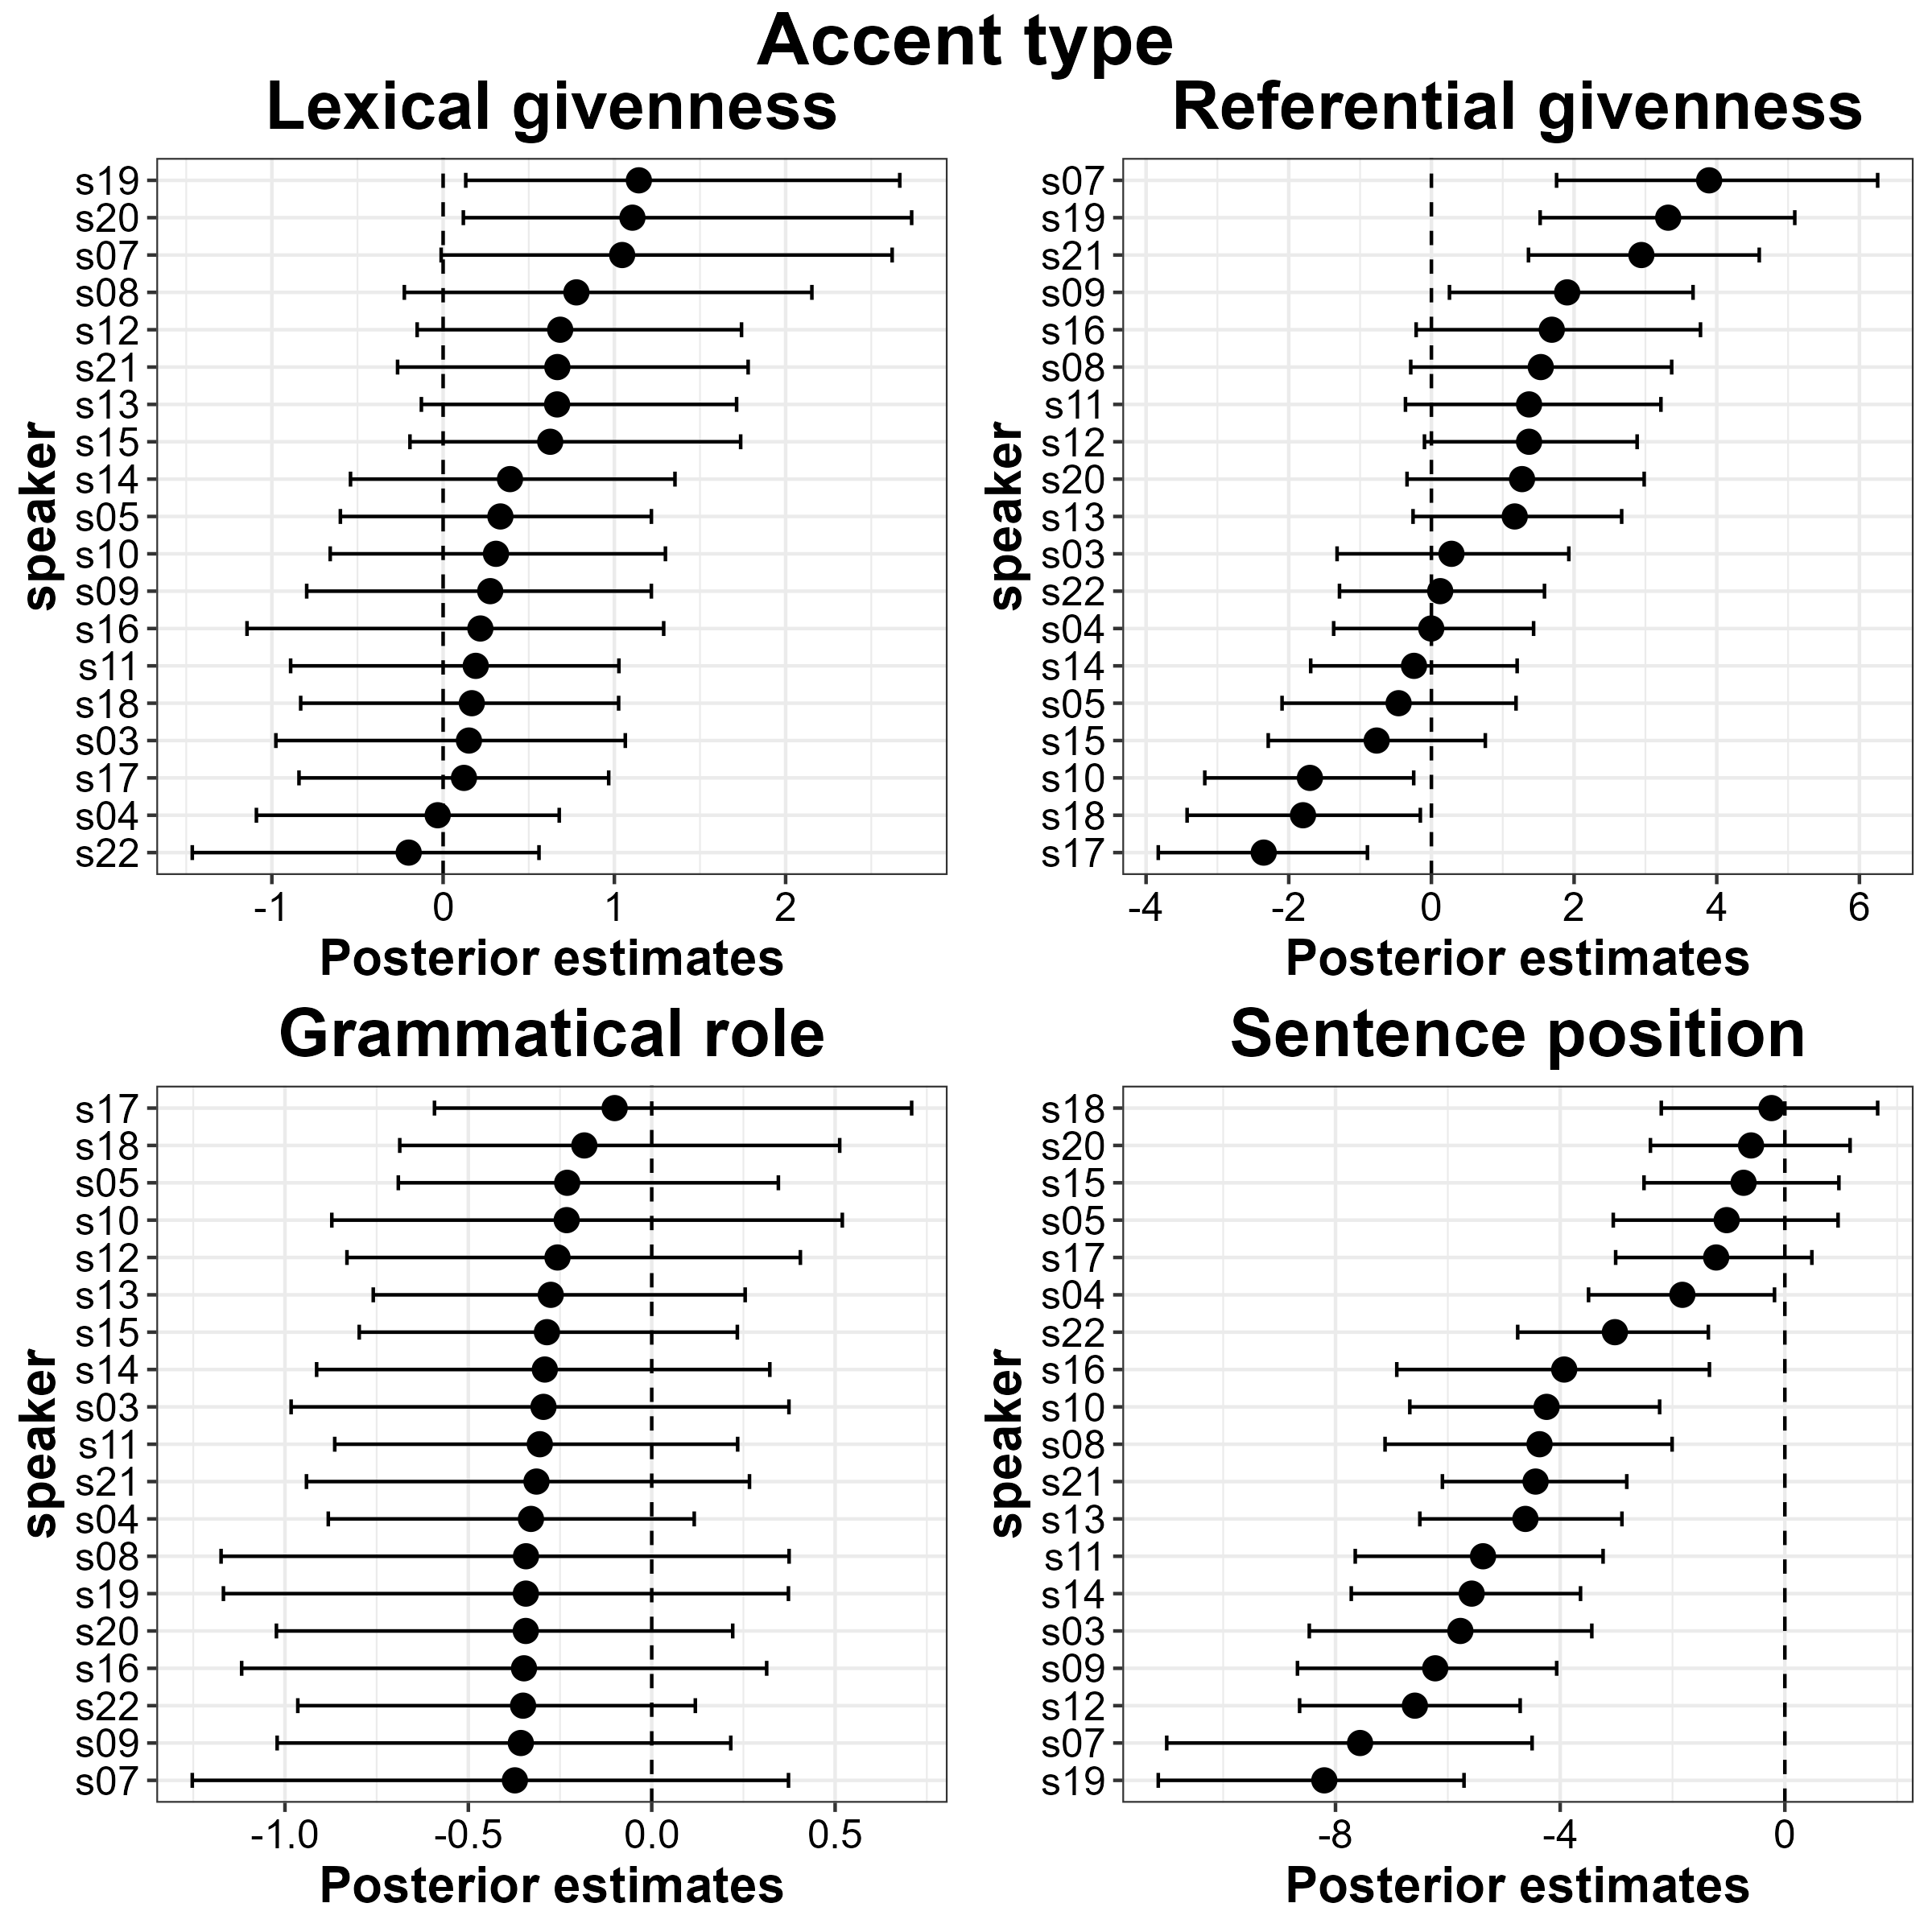
\includegraphics[scale = 0.5]{s2_accenttype_effects}
	\caption{Means and 90\% CrIs for the effects of lexical and referential givenness, grammatical role, and sentence position on accent type.}
	\label{fig:s2_accenttype_effects}
\end{figure}

To identify potential different strategies for the encoding of lexical and referential givenness, grammatical role, and sentence position via the continuous prosodic parameters, we run cluster analyses on the by-speaker random slopes extracted from the corresponding models (see Section \ref{sec:Production2 statistics} for details). For lexical givenness, the hierarchical cluster analysis suggests that a two cluster-solution is most appropriate for our data (silhouette width: 0.23). Cluster 1 contains twelve speakers and Cluster 2 contains seven speakers (see Figure \ref{fig:s2_clusters_lex}, left). Figure \ref{fig:s2_clusters_lex} (right) shows the average random slope values with 90\% CrIs for the effect of lexical givenness on the prosodic parameters per cluster. Here, a positive number indicates that l-new referents have a higher value than l-given referents in the parameter in question. The two clusters appear remarkably alike in their use of almost all parameters. The main difference between these two groups of speakers is the strength of encoding via syllable duration and periodic energy mass. Specifically, Cluster 2 marks a larger difference between l-new and l-given referents in terms of these two parameters. The same is true for F0 at CoM, word duration, and intensity, although the differences between the two clusters here are smaller. Overall, lexical givenness is thus very similarly encoded across speakers, which is supported by the low silhouette width value, indicating that there is only weak evidence for clustering potential in the data.

\begin{figure}
		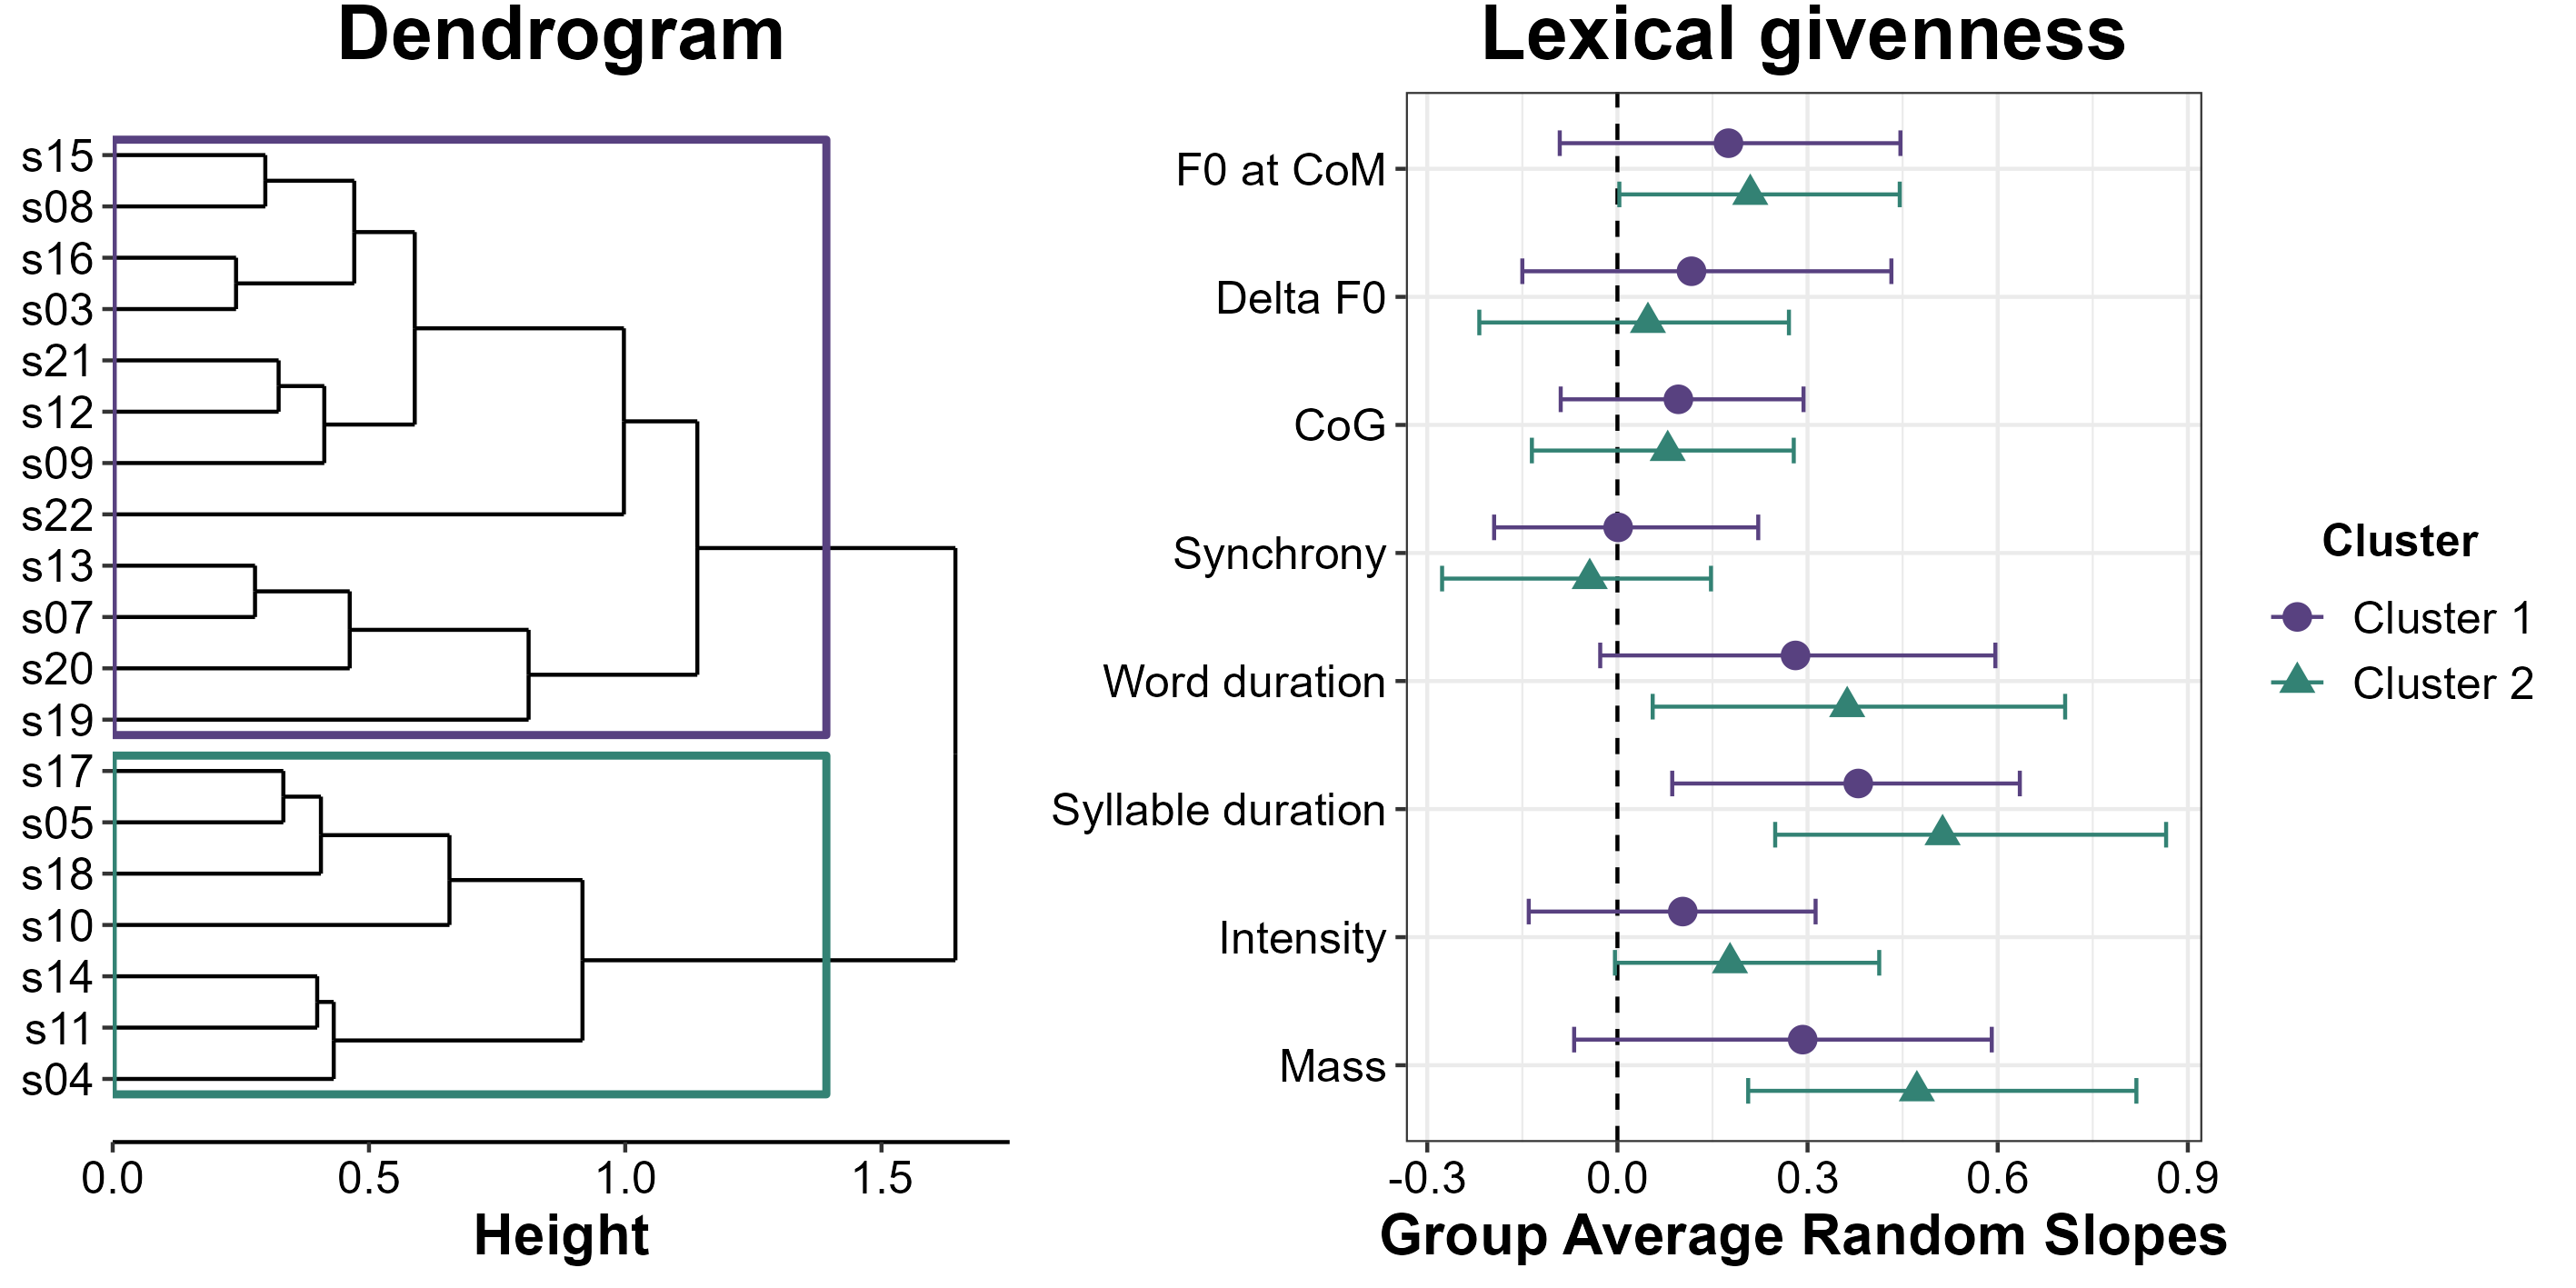
\includegraphics[scale = 0.5]{s2_clusters_lex}
	\caption{Results of cluster analysis for lexical givenness. Left: Dendrogram showing cluster affiliations of all speakers for lexical givenness. Right: Group averages and 90\% CrIs per cluster for each prosodic parameter.}
	\label{fig:s2_clusters_lex}
\end{figure}

Considering referential givenness, again two clusters of speakers emerge from the analysis (silhouette width: 0.34). Cluster 1 contains ten speakers while Cluster 2 contains nine speakers (see Figure \ref{fig:s2_clusters_ref}, left). Figure \ref{fig:s2_clusters_ref} (right) illustrates the characteristics of these two clusters. Here, the clusters converge on their use of word duration, syllable duration, intensity, and periodic energy mass. However, there appear to be differences in the modulation of F0 in r-new and r-given referents across the two clusters. In particular, Cluster 2 appears to produce r-new referents relatively consistently with higher F0 at the CoM and higher Delta F0 than r-given referents, whereas Cluster 1 does not make use of these two parameters in a reliable way. Meanwhile, Cluster 1 distinguishes more clearly between r-new and r-given referents in the F0 alignment, i.e., r-new referents are produced with lower CoG and lower synchrony values compared to r-given referents, while Cluster 2 only uses CoG in a similar way to a slightly lesser extent but not synchrony.

\begin{figure}
		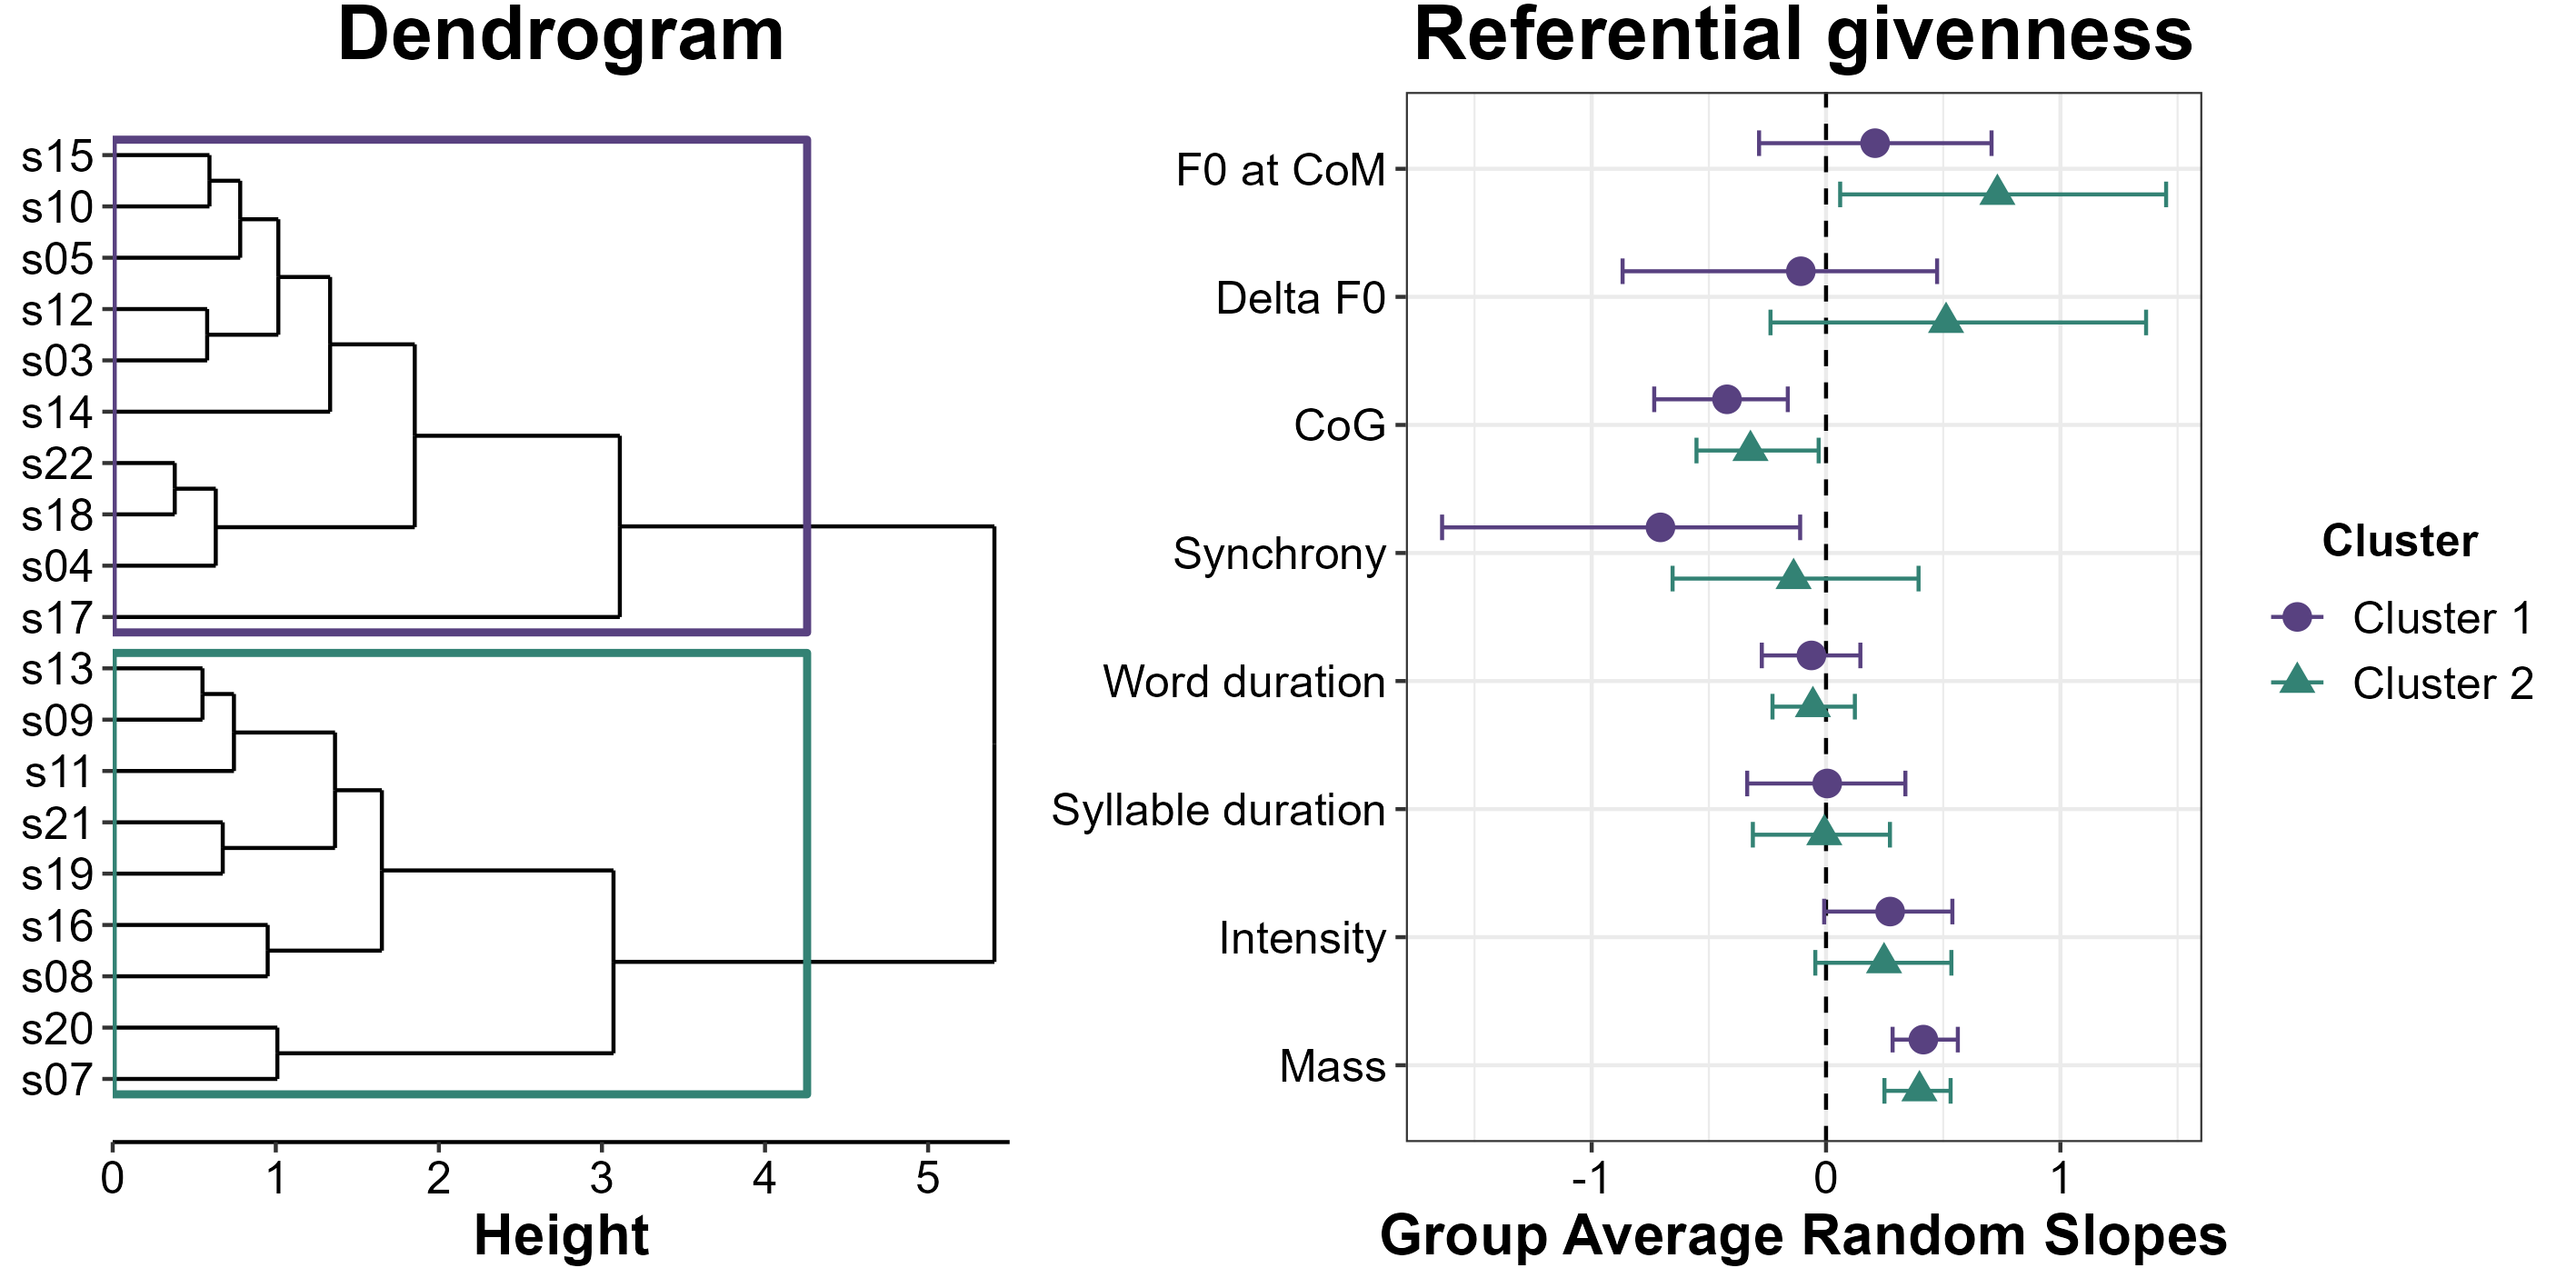
\includegraphics[scale = 0.5]{s2_clusters_ref}
	\caption{Results of cluster analysis for referential givenness. Left: Dendrogram showing cluster affiliations of all speakers for referential givenness. Right: Group averages and 90\% CrIs per cluster for each prosodic parameter.}
	\label{fig:s2_clusters_ref}
\end{figure}

Turning next to the encoding of grammatical role, the cluster analysis indicates that a split into three groups is most appropriate for our data (silhouette width: 0.37). Cluster 1 contains seven speakers, Cluster 2 four speakers, and Cluster 3 eight speakers (see Figure \ref{fig:s2_clusters_gramm}, left). Looking at the characteristics of these three clusters in Figure \ref{fig:s2_clusters_gramm} (right), clusters again behave very similarly in their use of most parameters, e.g., F0 at CoM, Delta F0, and periodic energy mass. The most obvious difference across clusters is in regards to CoG. While Cluster 3 barely modifies CoG between objects and subjects, Cluster 1 clearly produces an earlier CoG in objects, with Cluster 2 falling in between these two behaviors. 

\begin{figure}[t]
		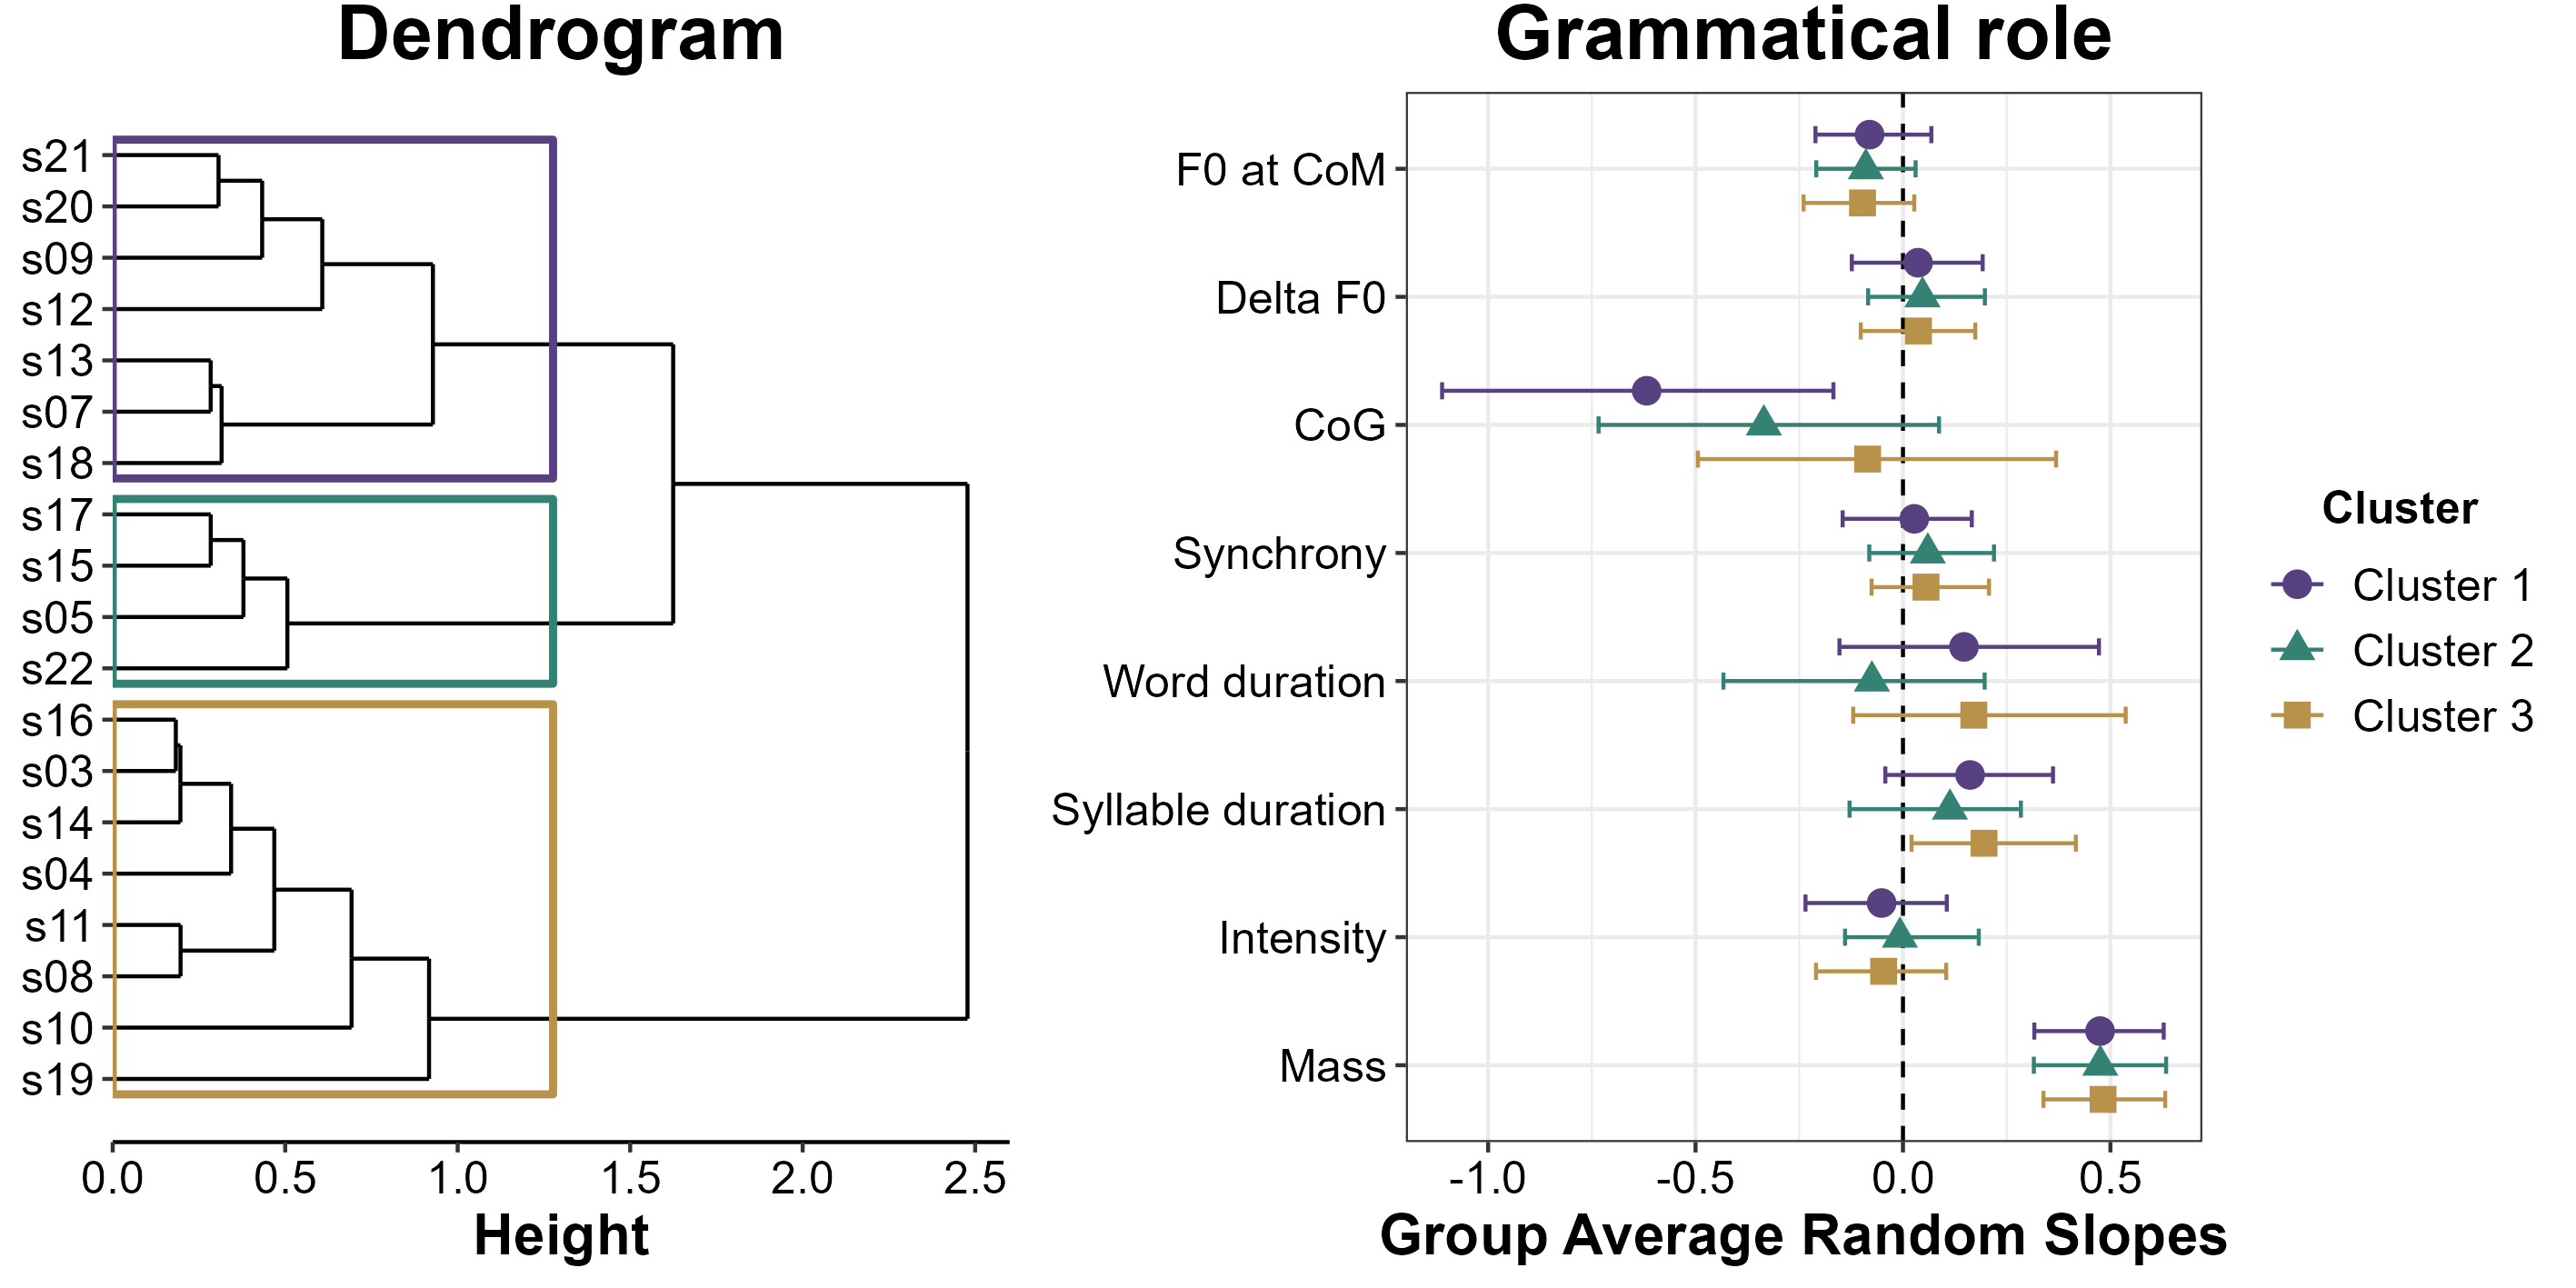
\includegraphics[scale = 0.5]{s2_clusters_gramm}
	\caption{Results of cluster analysis for grammatical role. Left: Dendrogram showing cluster affiliations of all speakers for grammatical role. Right: Group averages and 90\% CrIs per cluster for each prosodic parameter.}
	\label{fig:s2_clusters_gramm}
\end{figure}

Sentence position appears to give rise to the most variability across speakers, with the cluster analysis suggesting a partitioning into five clusters as optimal (silhouette width: 0.31). Accordingly, the individual clusters are smaller, with Cluster 1 containing four speakers, Cluster 2 five speakers, Cluster 3 six speakers, Cluster 4 three speakers, and Cluster 5 only one speaker (see Figure \ref{fig:s2_clusters_pos}, left). Judging from the CrIs' distance to the vertical zero line, it is evident that all clusters reliably differentiate between initial and medial target words in terms of synchrony, word duration, syllable duration, intensity, and periodic energy mass, albeit to differing extents (see Figure \ref{fig:s2_clusters_pos}, right). Nevertheless, there is some variability with regard to F0 at CoM, Delta F0, and CoG. Of these three, Cluster 1 appears to only use CoG, Cluster 2 and 3 use F0 at CoM and Delta F0, and Cluster 4 and 5 use all three to encode sentence position prosodically. There are also more gradient differences across these clusters, with Cluster 2 producing generally larger differences between initial and medial words than Cluster 3, and Cluster 5 (i.e., speaker s09) producing larger differences than Cluster 4.

\begin{figure}
		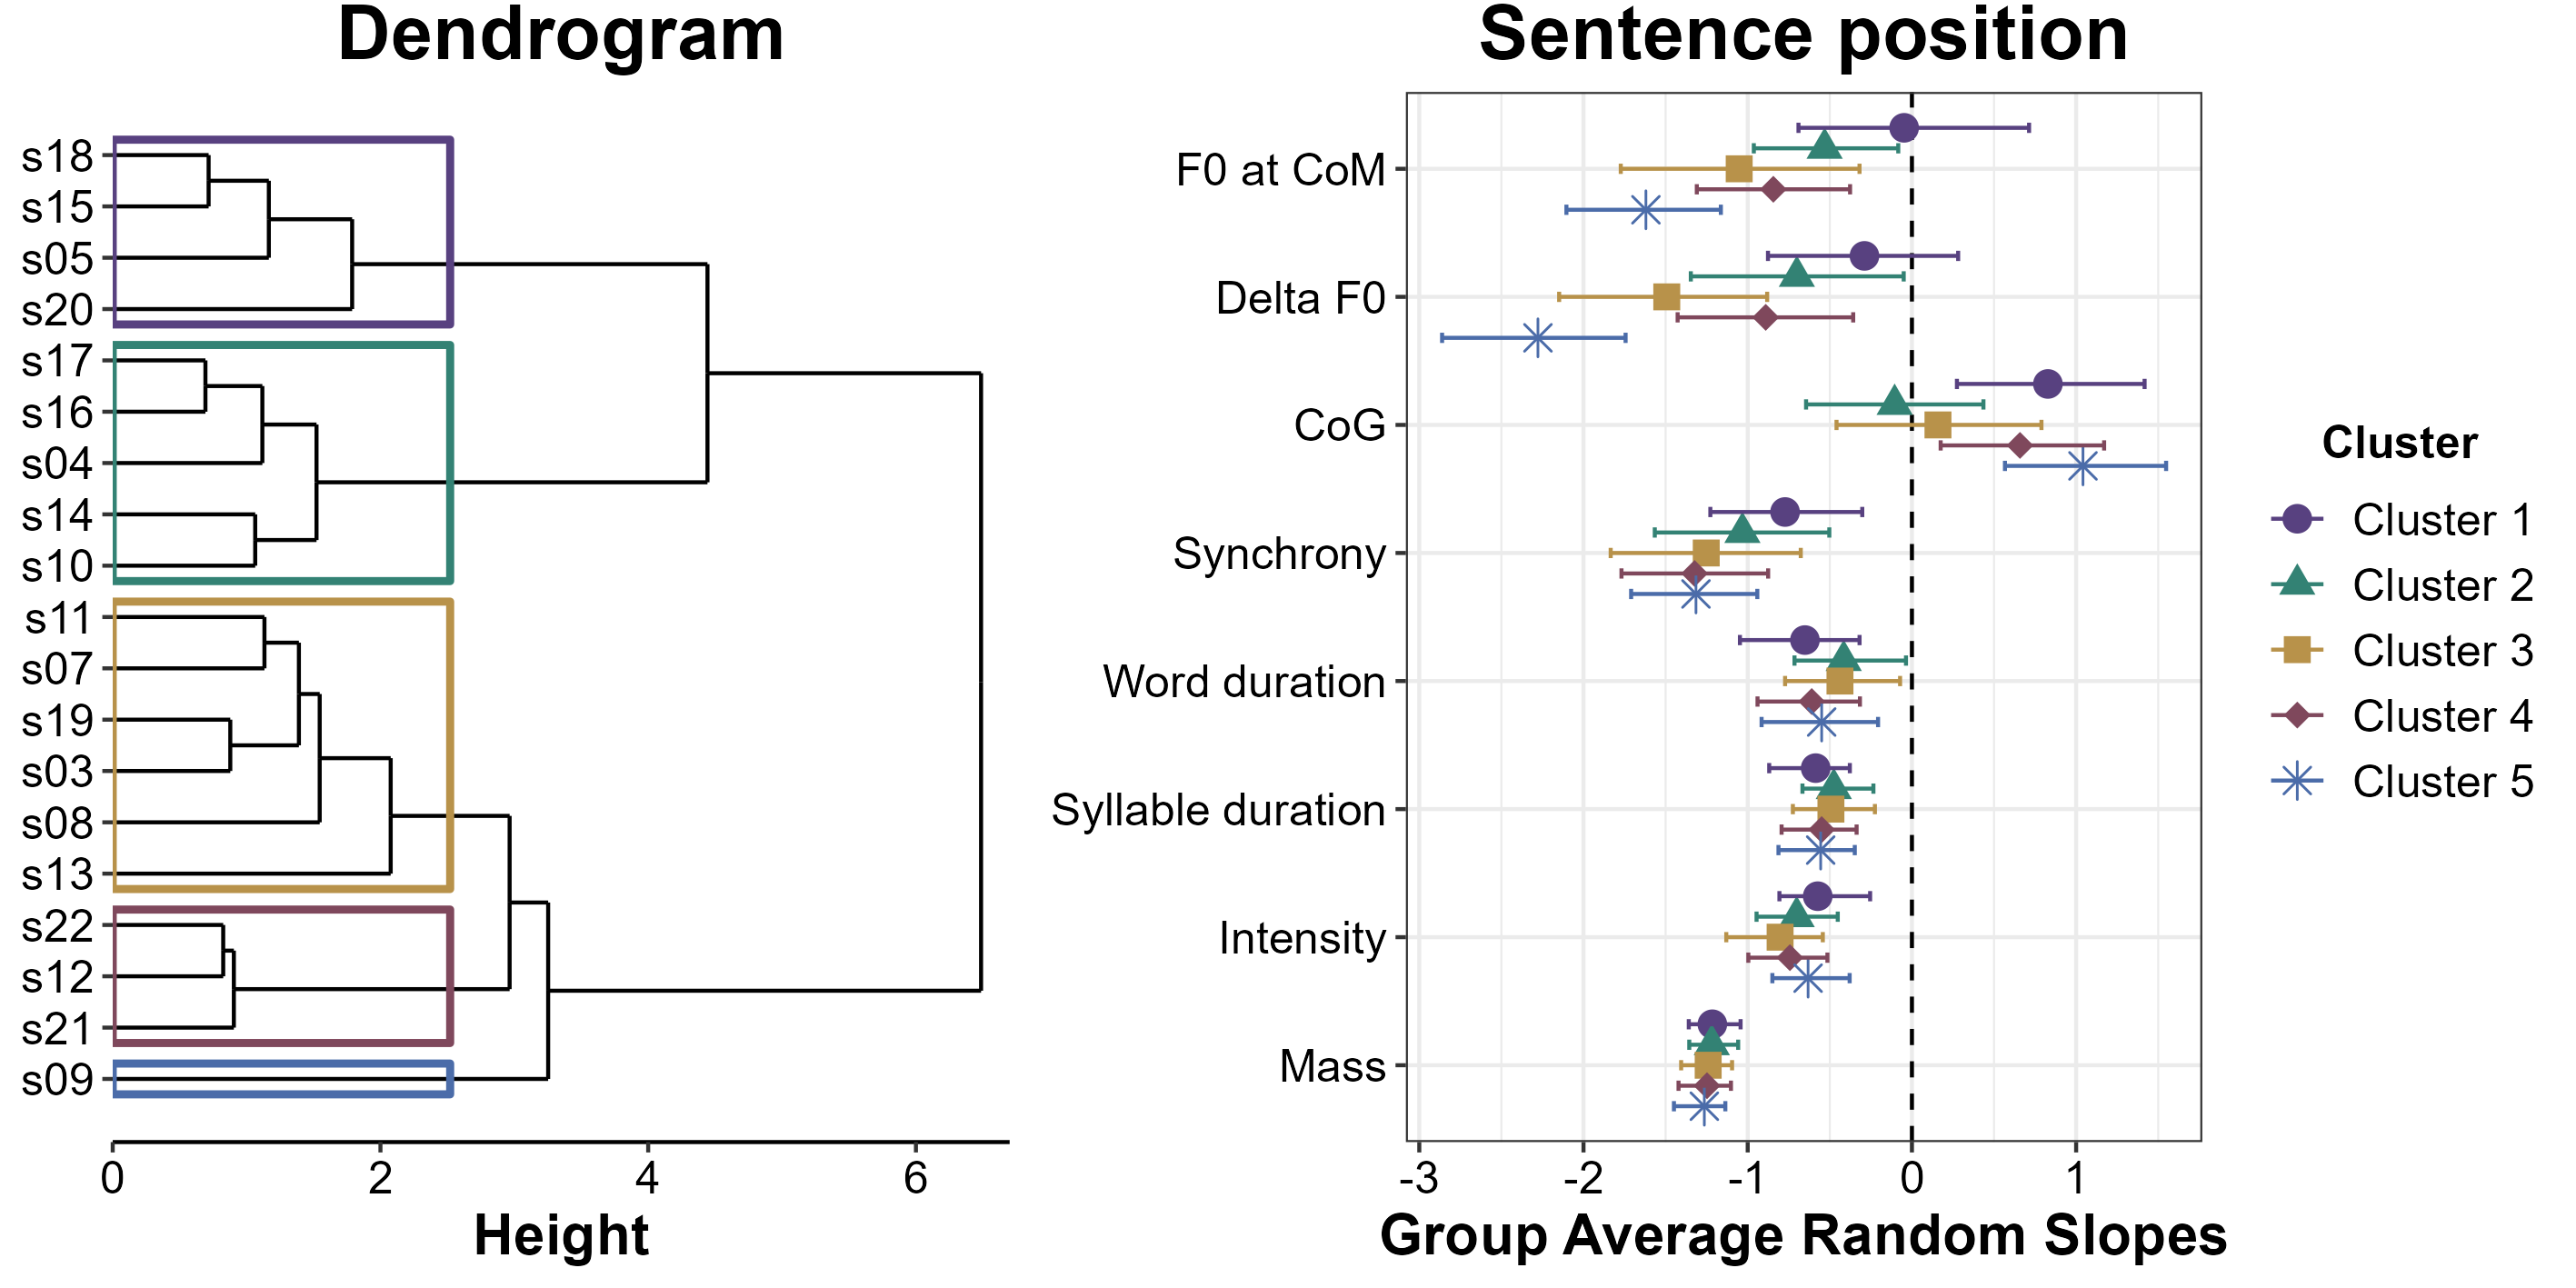
\includegraphics[scale = 0.5]{s2_clusters_pos}
	\caption{Results of cluster analysis for sentence position. Left: Dendrogram showing cluster affiliations of all speakers for sentence position. Right: Group averages and 90\% CrIs per cluster for each prosodic parameter.}
	\label{fig:s2_clusters_pos}
\end{figure}

To integrate the findings of the categorical and continuous parameters, we plot the number of speakers using or not using accent status and accent type as cues to each of the semantic-pragmatic and syntactic factors under investigation by their cluster affiliations. We classify a speaker as a user of accent status or type when the 90\% CrI of their corresponding random slope does not include zero (see Figures \ref{fig:s2_accentstatus_effects} and \ref{fig:s2_accenttype_effects}). First, lexical givenness is reliably encoded by accent status and accent type only by a few speakers, so that it is difficult to identify systematic behavior by any of the two clusters (see Figure \ref{fig:s2_accent_statustype_bycluster_lex}). In Cluster 1, there are two speakers using accent status and two other speakers using accent type to cue lexical givenness. Similarly, in Cluster 2, two speakers use accent status, however, none are users of accent type. Proportionally, with Cluster 2 containing fewer speakers overall, speakers affiliated with Cluster 2 are more likely to use accent status than speakers in Cluster 1. This finding corresponds to the observation that Cluster 2 also makes stronger use of the continuous parameters than Cluster 1, especially those related to duration and intensity. For accent type, the relation is reversed, with more speakers in Cluster 1 making use of different accent types to mark lexical givenness. Overall, the two clusters are very similar in their encoding of lexical givenness in both their modulation of categorical and continuous prosodic parameters. 

\begin{figure}
		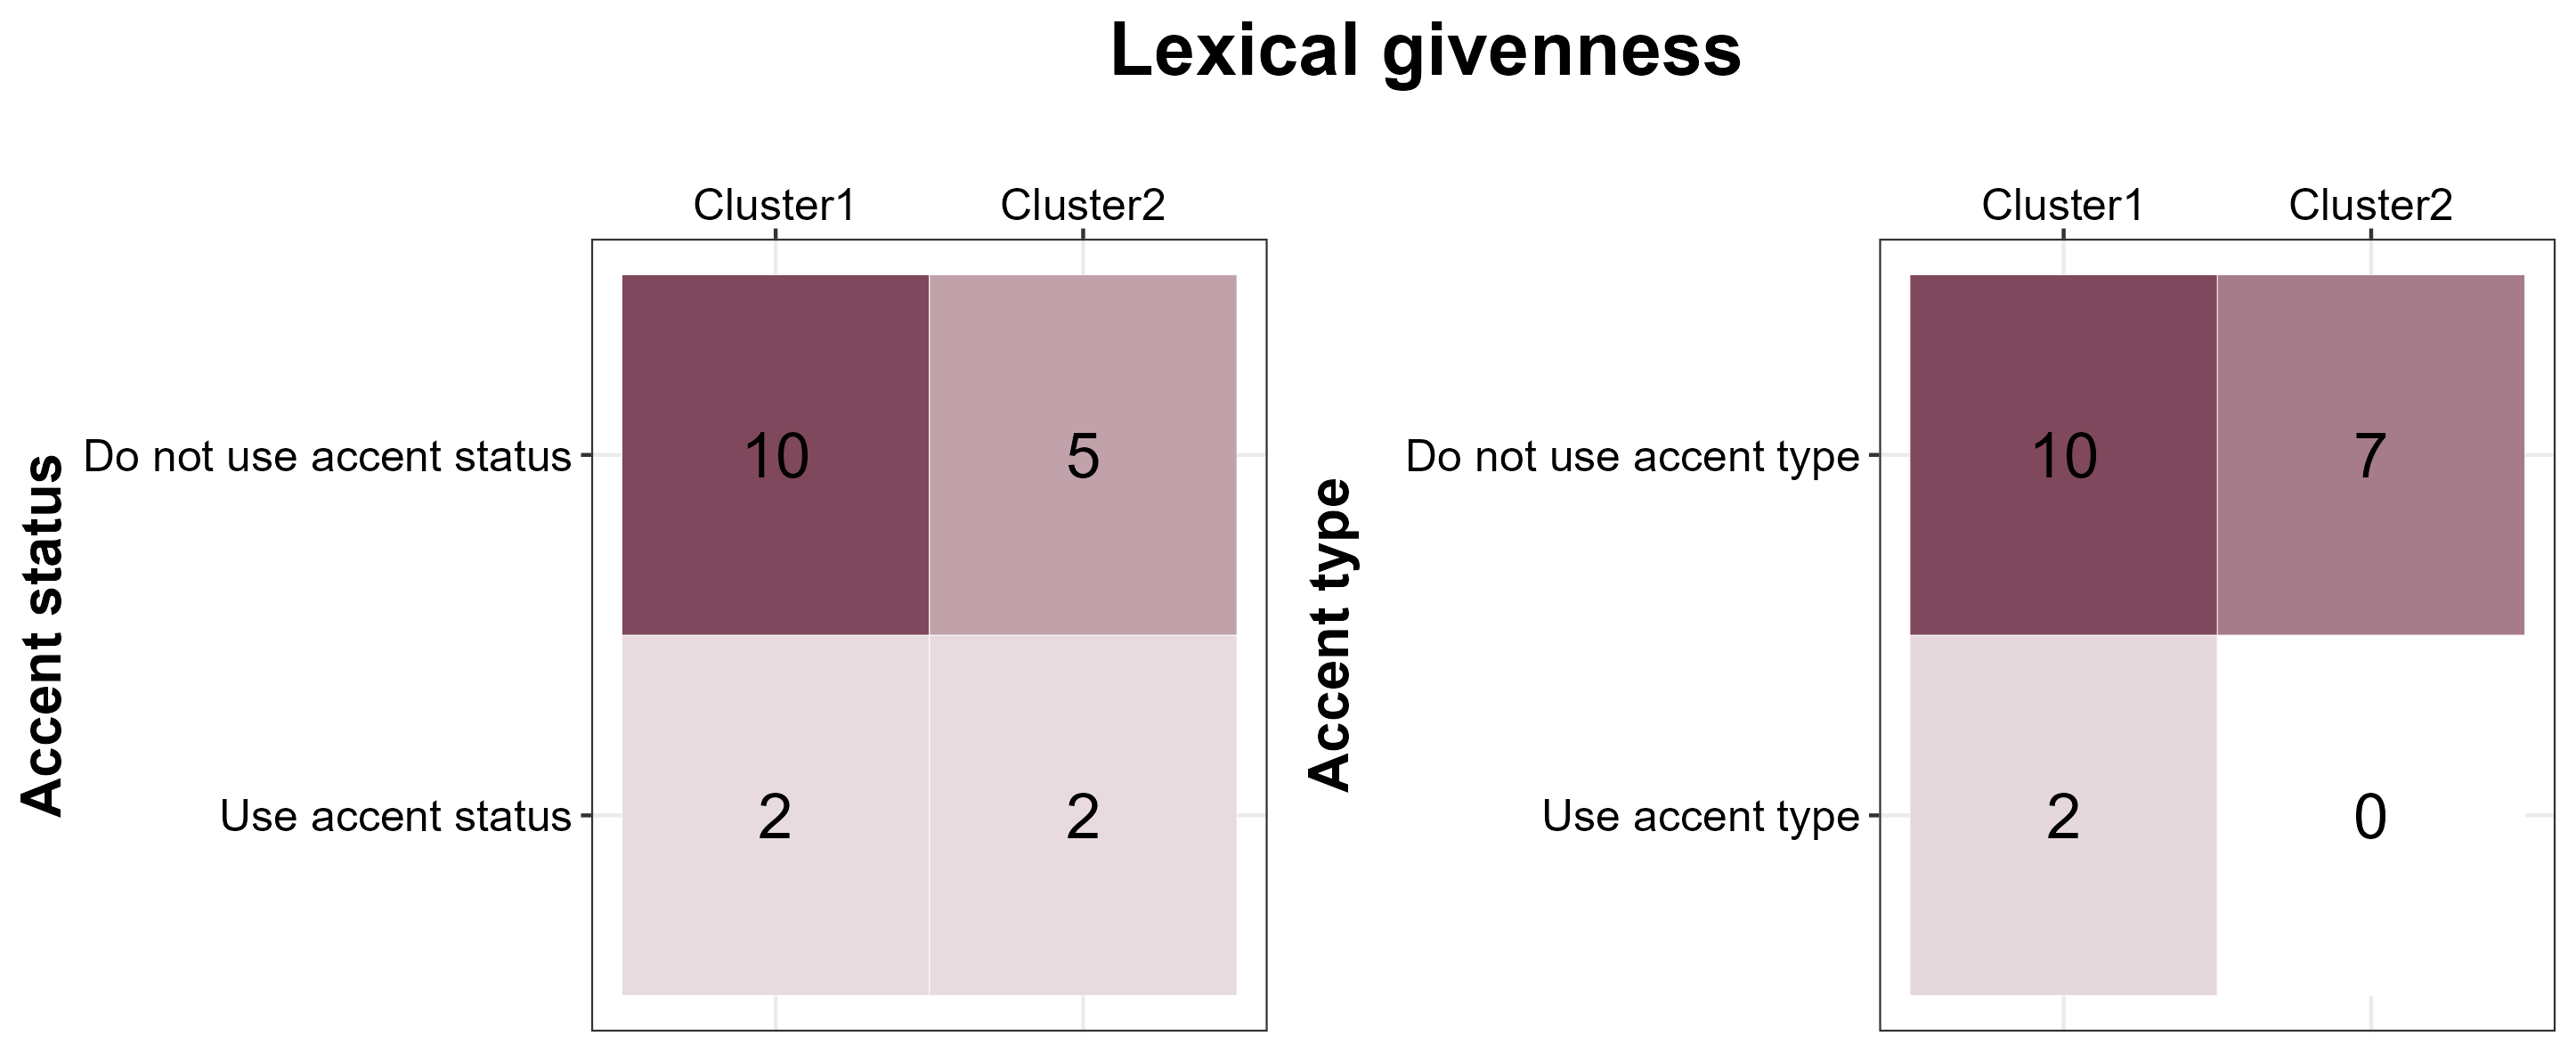
\includegraphics[scale = 0.5]{s2_accent_statustype_bycluster_lex}
	\caption{Plot showing the number of speakers using accent status (left) and accent type (right) to encode lexical givenness as a function of their cluster.}
	\label{fig:s2_accent_statustype_bycluster_lex}
\end{figure}

For referential givenness, a more interesting picture emerges. As evident from Figure \ref{fig:s2_accent_statustype_bycluster_ref}, most speakers reliably use accent status as a cue to referential givenness, regardless of their cluster affiliation. In contrast, none of the speakers in Cluster 1 uses more prominent accent types to mark r-new words. However, three speakers from this cluster produce the opposite pattern, with more prominent accent types on r-given words. This pattern is unattested in Cluster 2. Instead, about half of the speakers in Cluster 2 do not use accent type to mark referential givenness, but the other half makes use of accent type in the expected direction. This latter observation is also reflected in some of the continuous F0 measures, most notably F0 at CoM and Delta F0, which are used to a larger extent by Cluster 2 than by Cluster 1.

\begin{figure}
		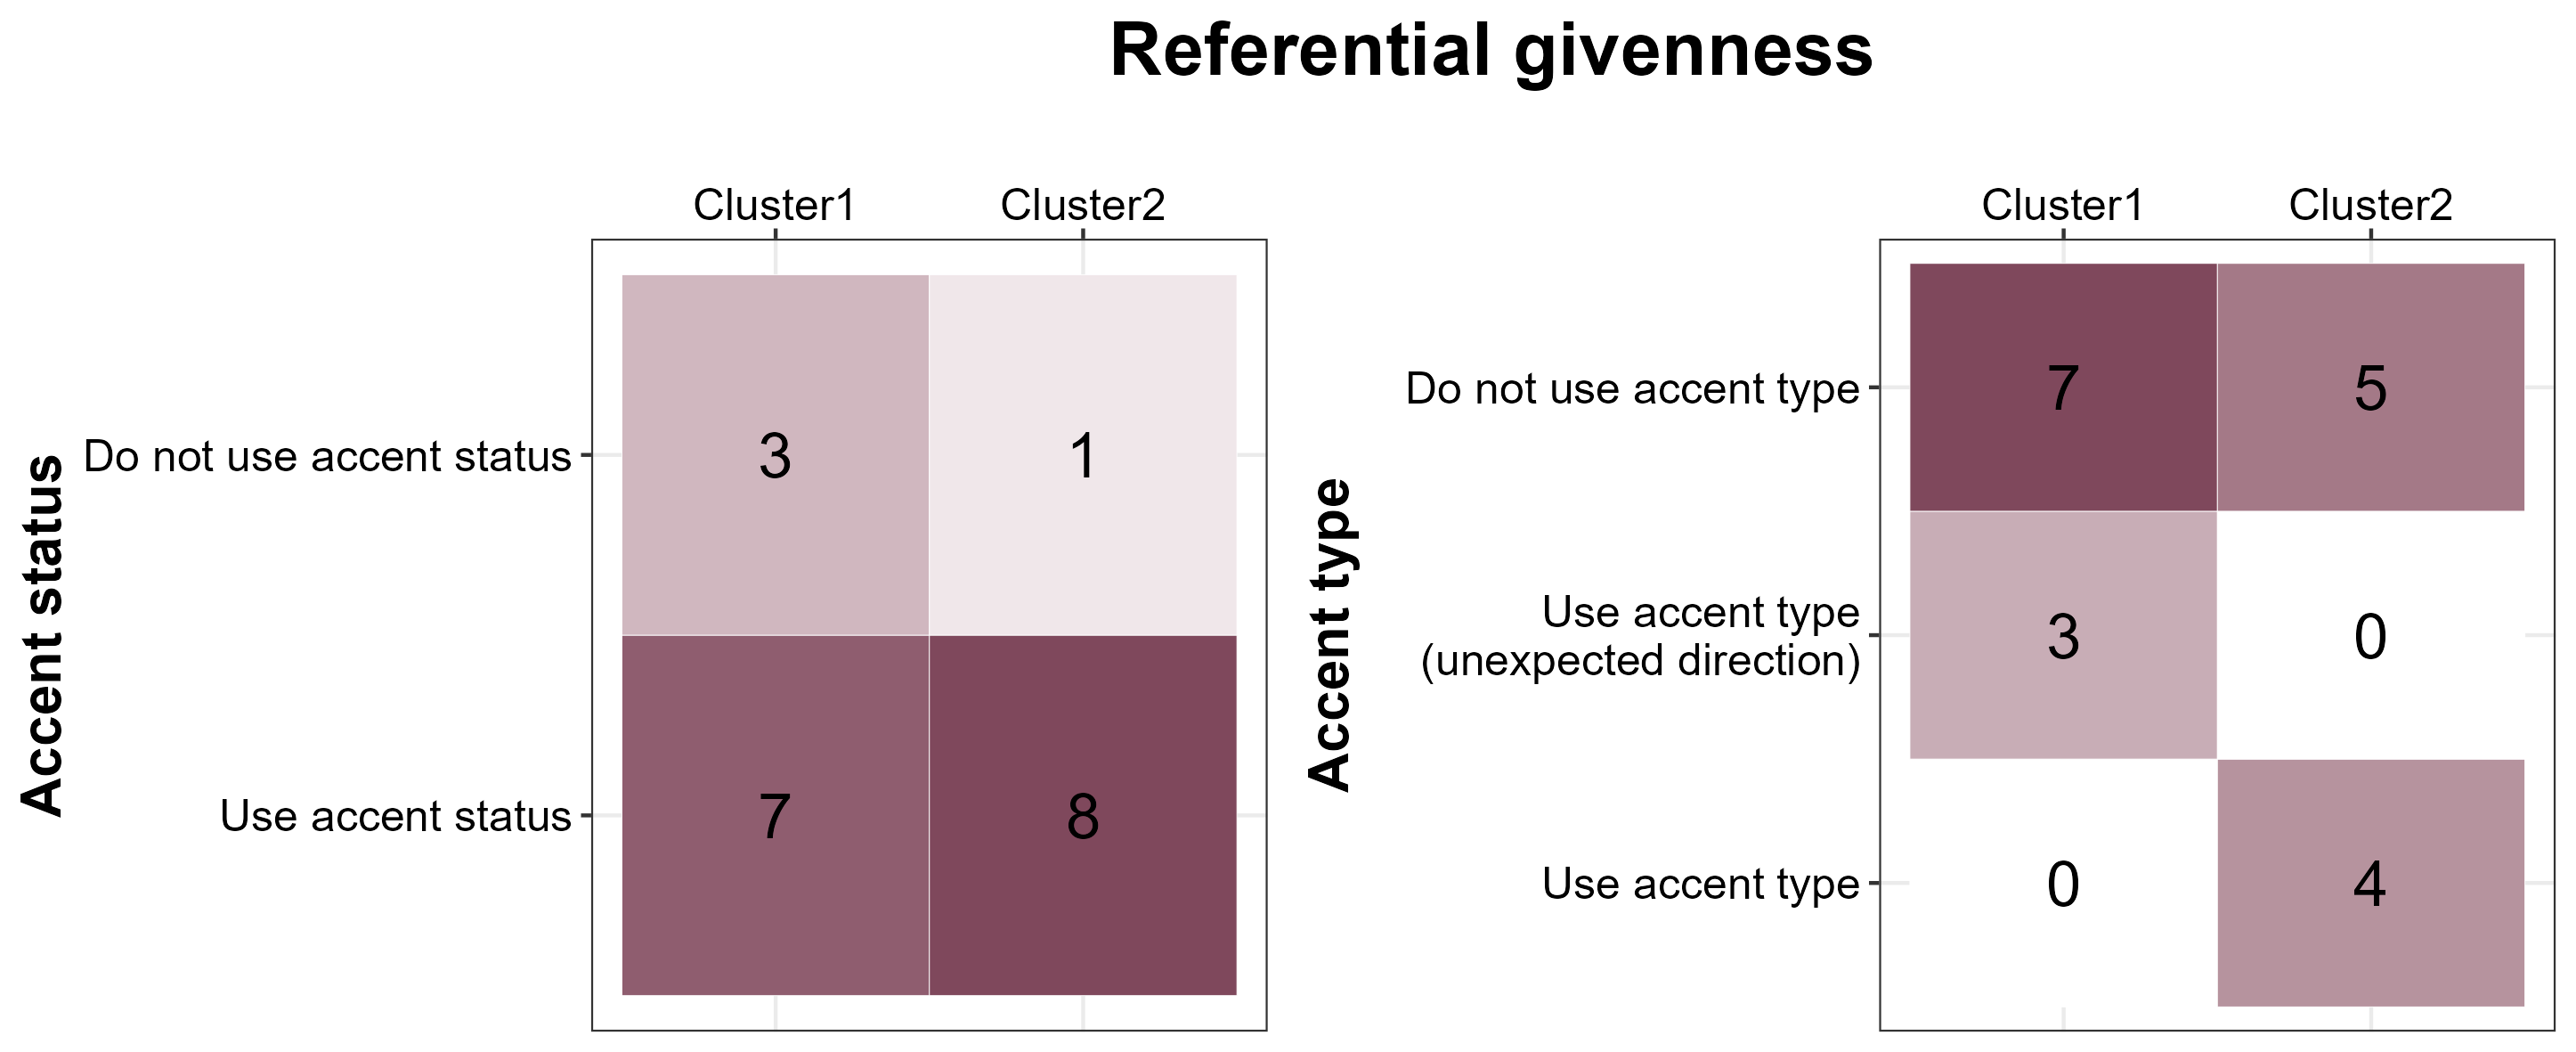
\includegraphics[scale = 0.5]{s2_accent_statustype_bycluster_ref}
	\caption{Plot showing the number of speakers using accent status (left) and accent type (right) to encode referential givenness as a function of their cluster.}
	\label{fig:s2_accent_statustype_bycluster_ref}
\end{figure}

The three clusters that emerged from the analysis of the encoding of grammatical role pattern very clearly with regard to their use of accent status and accent type (see Figure \ref{fig:s2_accent_statustype_bycluster_gramm}). While Cluster 1 and Cluster 2 rely on accent status but not accent type to mark objects as more prominent than subjects, the majority of speakers in Cluster 3 uses neither of the categorical parameters to this end. In contrast to the findings on lexical and referential givenness, these observations do not directly relate to the findings with regard to the continuous parameters, suggesting that categorical and continuous parameters may also act independently to some degree. 

\begin{figure}[t]
		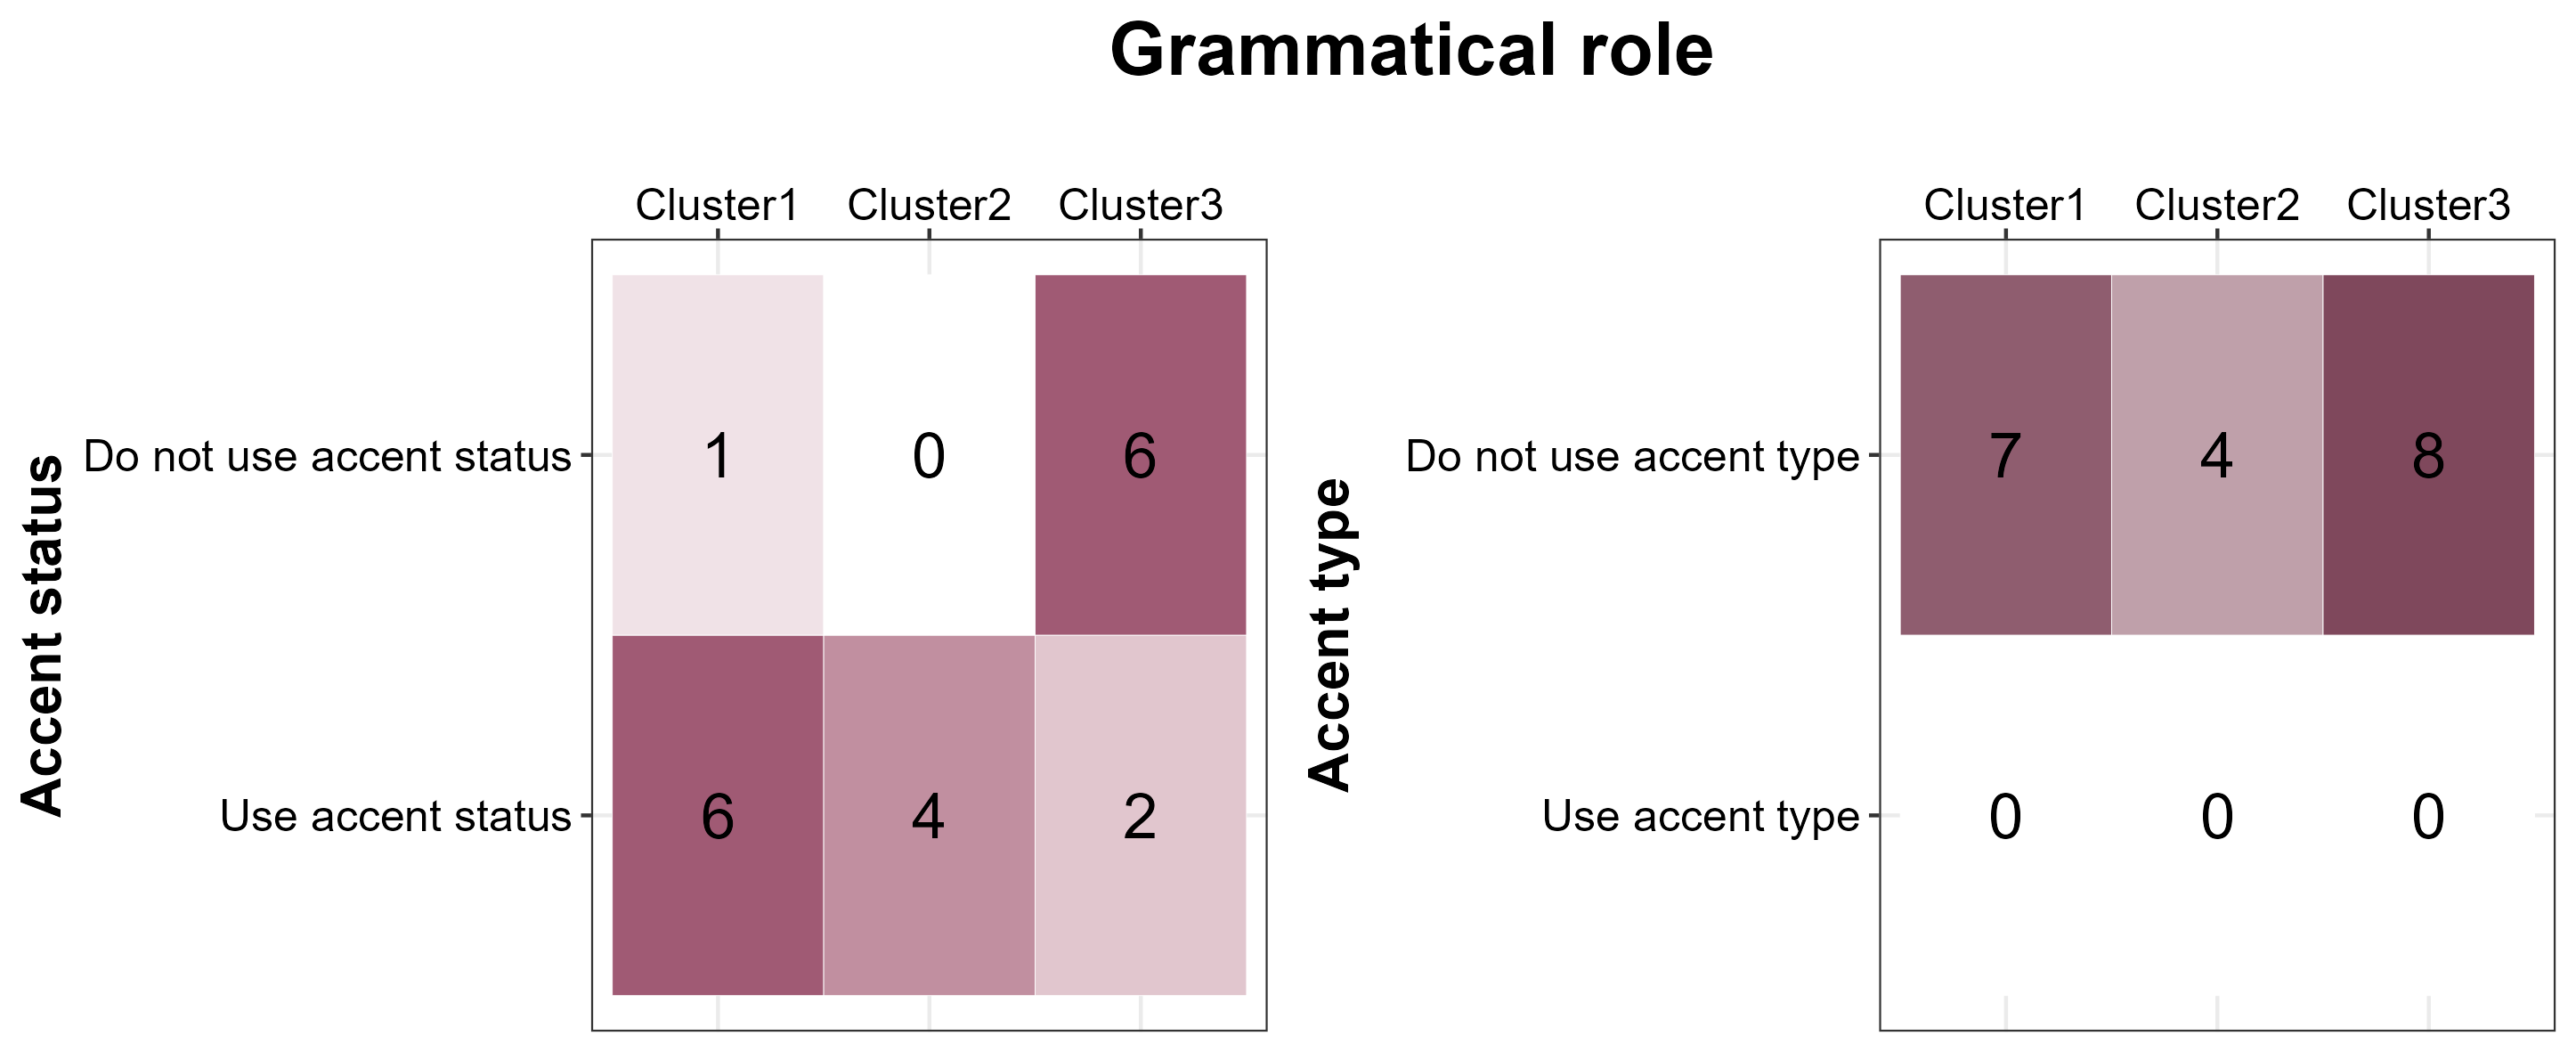
\includegraphics[scale = 0.5]{s2_accent_statustype_bycluster_gramm}
	\caption{Plot showing the number of speakers using accent status (left) and accent type (right) to encode grammatical role as a function of their cluster.}
	\label{fig:s2_accent_statustype_bycluster_gramm}
\end{figure}

Finally, for sentence position, a mostly complementary pattern emerges across clusters (see Figure \ref{fig:s2_accent_statustype_bycluster_pos}). While Cluster 1 uses accent status but not accent type to mark initial target words as more prominent than medial words, the reverse is true for Cluster 2, Cluster 3, and Cluster 4, where the majority of speakers use accent type but not accent status. The single speaker in Cluster 5 provides an exception to the complementary pattern, making use of both accent status and accent type. In line with this observation, the speaker in Cluster 5 also distinguishes most clearly between the initial and medial positions in terms of continuous parameters. The use of accent type correlates nicely with higher mean F0 at CoM and Delta F0 for initial words produced by speakers in Cluster 2, Cluster 3, Cluster 4, and Cluster 5 compared to Cluster 1.

\begin{figure}[t]
		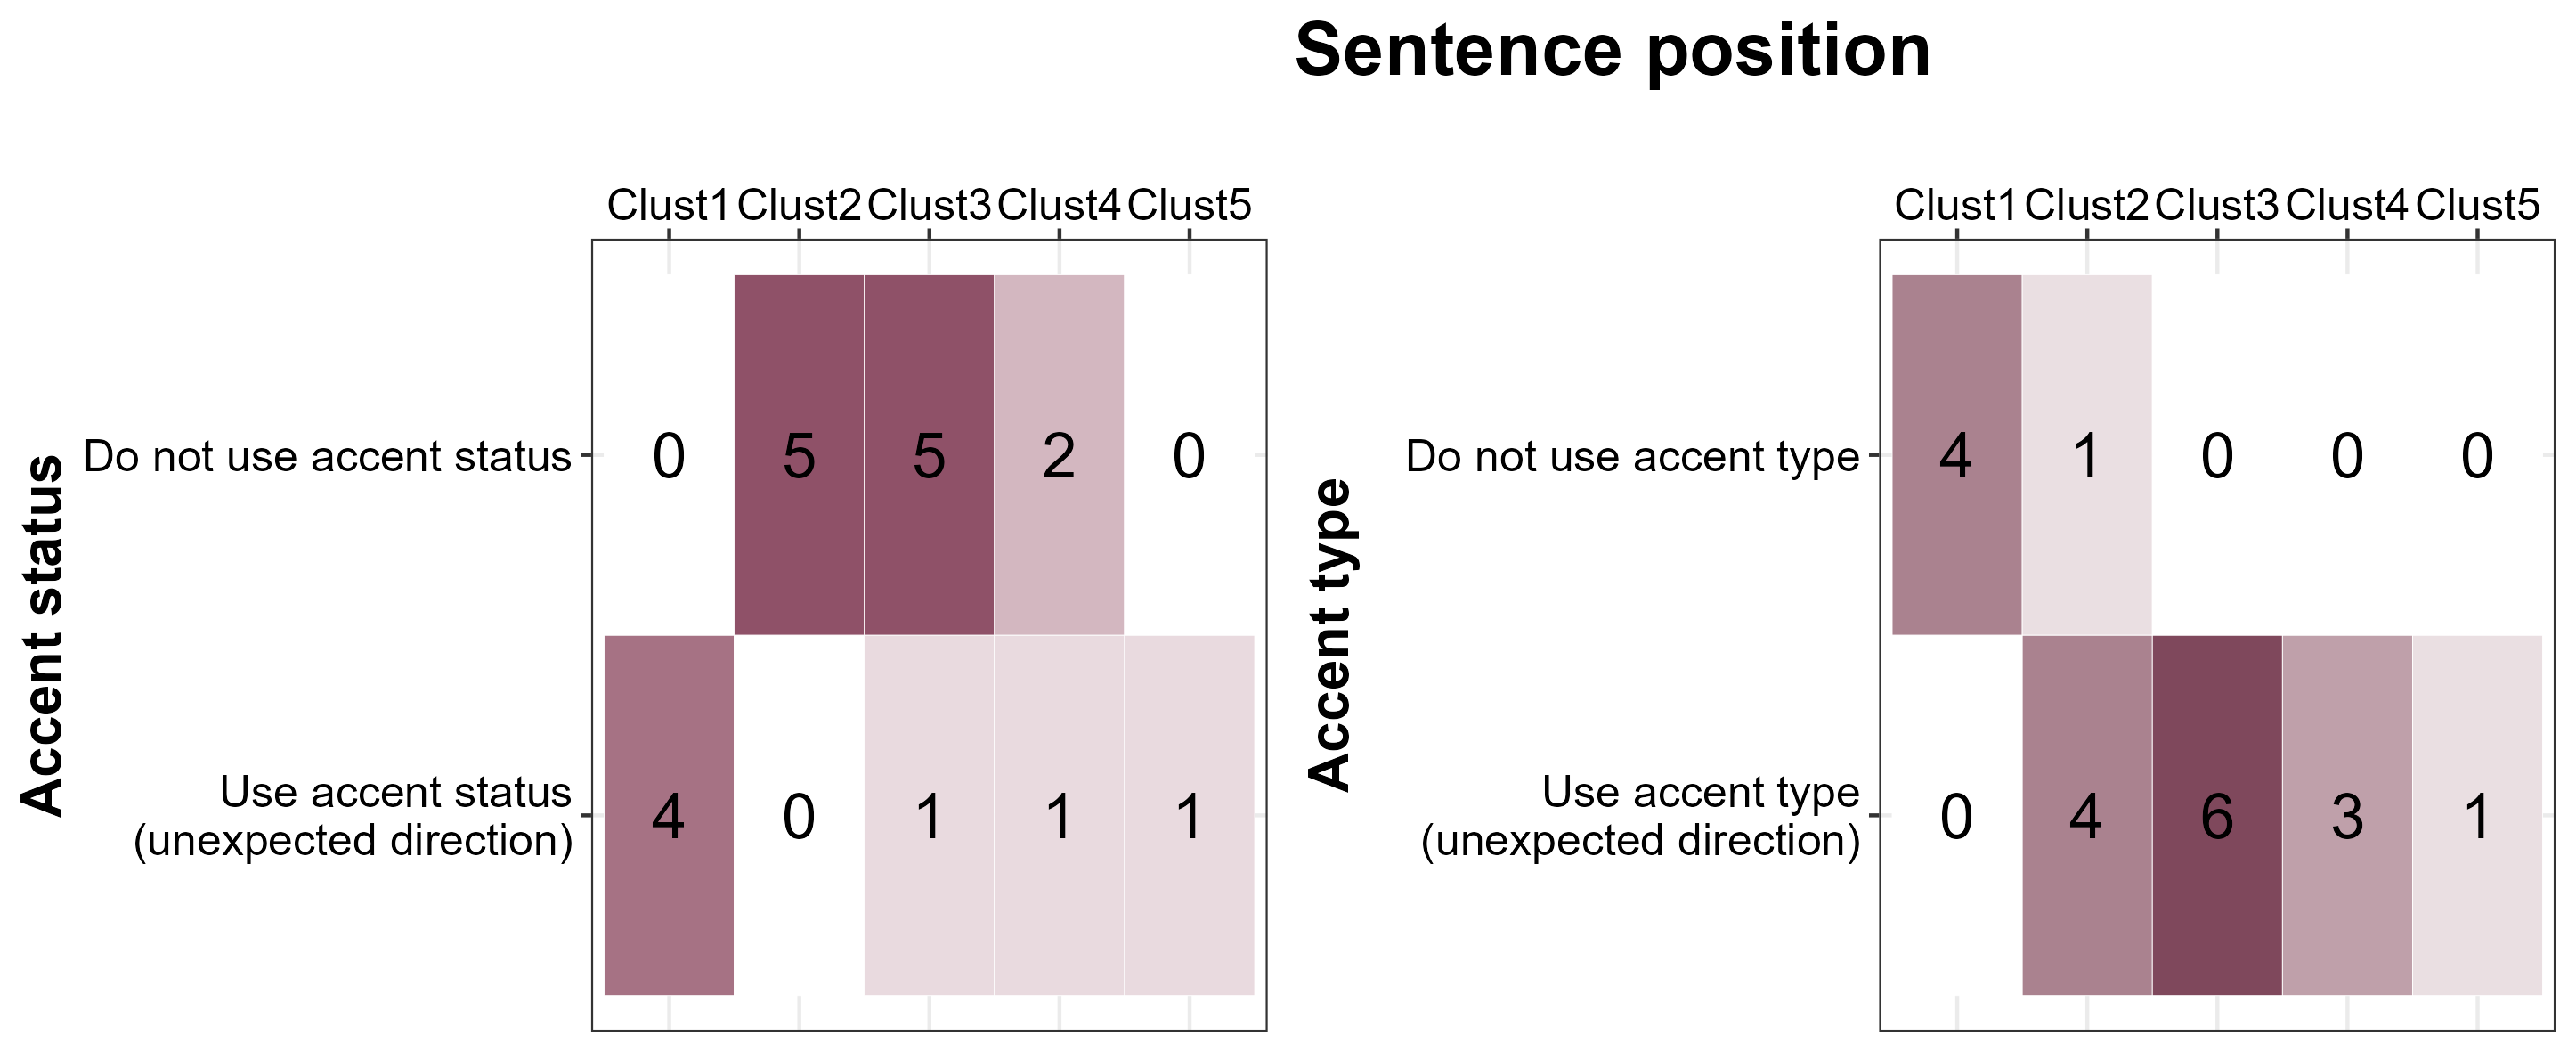
\includegraphics[scale = 0.5]{s2_accent_statustype_bycluster_pos}
	\caption{Plot showing the number of speakers using accent status (left) and accent type (right) to encode sentence position as a function of their cluster.}
	\label{fig:s2_accent_statustype_bycluster_pos}
\end{figure}

Generally, continuous parameters reflect categorical ones relatively well, so that clustering performed on the continuous parameters corresponds to patterns in terms of categorical parameters across speakers.

Before turning to potential effects of communicative skill, we briefly note on the sociodemographic characteristics of the speakers in the reported clusters. For lexical givenness, we identified two clusters, the weaker encoders (Cluster 1) and the stronger encoders (Cluster 2). Speakers in Cluster 1 are on average slightly older than in Cluster 2, relatively balanced in gender, and more likely from the north of Germany. Speakers in Cluster 2 are slightly younger, more likely female than male, and more balanced in terms of region of origin (see Table \ref{table:s3_sociodemographics_lexical}). 

\begin{table}[b]
\begin{tabularx}{\textwidth}{lXX}
\lsptoprule
\multicolumn{3}{c}{Lexical givenness} \\ \hline
                 & Cluster 1 \newline n = 12     & Cluster 2 \newline n = 7    \\ \hline
Age (median)     & 26                     & 24                     \\
Gender           & 58\% female, 42\% male & 86\% female, 14\% male \\
Region of origin & 83\% north, 17\% south & 57\% north, 43\% south \\
\lspbottomrule
\end{tabularx}
\caption{Sociodemographic characteristics of the two clusters using different strategies to encode lexical givenness.}
\label{table:s3_sociodemographics_lexical}
\end{table}

For referential givenness, we also observed two different strategies. Speakers in Cluster 1 relied more on F0 alignment to encode this meaning contrast, speakers in Cluster 2 relied more on F0 scaling. Cluster 1 consists of slightly younger, more female speakers, who are equally likely from the north or south of Germany. Speakers in Cluster 2 are slightly older, relatively balanced in gender, and exclusively from the north (see Table \ref{table:s3_sociodemographics_referential}). 

\begin{table}[]
\begin{tabularx}{\textwidth}{lXX}
\lsptoprule
\multicolumn{3}{c}{Referential givenness} \\ \hline
                 & Cluster 1 \newline n = 10   & Cluster 2 \newline n = 9     \\ \hline
Age (median)     & 24                     & 27                     \\
Gender           & 90\% female, 10\% male & 44\% female, 56\% male \\
Region of origin & 50\% north, 50\% south & 100\% north, 0\% south \\
\lspbottomrule
\end{tabularx}
\caption{Sociodemographic characteristics of the two clusters using different strategies to encode referential givenness.}
\label{table:s3_sociodemographics_referential}
\end{table}

Three different strategies were identified in the prosodic marking of grammatical role, which were nevertheless relatively similar. The largest difference related to CoG, where Cluster 1 produced the strongest distinction and Cluster 3 the weakest. In terms of sociodemographic characteristics, median age is comparable across clusters, gender distribution is balanced in Cluster 1, slightly skewed toward female in Cluster 3, and exclusively female in Cluster 2 (see Table \ref{table:s3_sociodemographics_gramm}). Region of origin is balanced in Cluster 2, but more speakers are from the north than the south in Cluster 1 and Cluster 3. 

\begin{table}[]
\begin{tabularx}{\textwidth}{lXXX}
\lsptoprule
\multicolumn{4}{c}{Grammatical role} \\ \hline
                 & Cluster 1 \newline n = 7    & Cluster 2 \newline n = 4  &   Cluster 3 \newline n = 8\\ \hline
Age (median)     & 25                     & 25                    & 26\\
Gender           & 57\% female, \newline 43\% male & 100\% female, \newline 0\% male & 63\% female, \newline 37\% male\\
Region of origin & 86\% north, \newline 14\% south & 50\% north, \newline 50\% south & 75\% north, \newline 25\% south\\
\lspbottomrule
\end{tabularx}
\caption{Sociodemographic characteristics of the three clusters using different strategies to encode grammatical role.}
\label{table:s3_sociodemographics_gramm}
\end{table}

Finally, for sentence position we identified five clusters, which complicates the process of looking at averaged sociodemographic characteristics even further because the number of speakers in each cluster is relatively small. We report age, gender, and region distributions for completeness in Table \ref{table:s3_sociodemographics_position} but refrain from further description in light of the small sample sizes and the gradient prosodic differences observed for this factor.

\begin{table}[]
\begin{tabularx}{\textwidth}{XXXXXX}
\lsptoprule
\multicolumn{6}{c}{Sentence position} \\ \hline
                 & Cluster 1 \newline n = 4    & Cluster 2 \newline n = 5 &   Cluster 3 \newline n = 6 &   Cluster 4 \newline n = 3 &   Cluster 5 \newline n = 1 \\ \hline
Age \newline (median)     & 25                     & 24                    & 25 & 26 & 31\\
Gender           & 100\% f., \newline 0\% m. & 80\% f., \newline 20\% m. & 33\% f., \newline 67\% m. & 100\% f., \newline 0\% m. & male\\
Region \newline of \newline origin & 50\% north, \newline 50\% south & 60\% north, \newline 40\% south & 100\% north, \newline 0\% south & 67\% north, \newline 33\% south & north\\
\lspbottomrule
\end{tabularx}
\caption{Sociodemographic characteristics of the five clusters using different strategies to encode position.}
\label{table:s3_sociodemographics_position}
\end{table}

\subsection{The moderating effect of communicative skill}

After investigating the nature of individual variability in the prosodic encoding of lexical and referential givenness, grammatical role, and sentence position, we turn to a potential reason for such differences, namely, communicative skill. Participants could score between 0 and 10 points in the self-reported communicative skill questionnaire, where a score of 0 indicates the lowest communicative skill and 10 the highest. Participants in the present study scored between 3 and 10 points with a mean of 7.3 (SD = 2.1), indicating relatively high communicative skill among most participants. Note that in the subsequent figures, communicative skill is always presented as a centered variable, that is, zero corresponds to the mean across all participants. In the following, we take a look at the interaction effects of communicative skill with the four variables lexical givenness, referential givenness, grammatical role, and sentence position. Generally, we expect speakers with higher communicative scores to encode any contrast more clearly than speakers with lower communicative scores, i.e., in the subsequent plots, the shaded CrIs should be farther removed from the dashed horizontal line (marking no difference) for higher communicative scores. In addition, wider CrIs indicate more uncertainty with regard to the interaction of communicative score and the prosodic parameter in question, which may indicate that speakers with similar communicative scores behave differently, i.e., there is individual variability that is not explained by the communicative score variable. 

\begin{figure}
		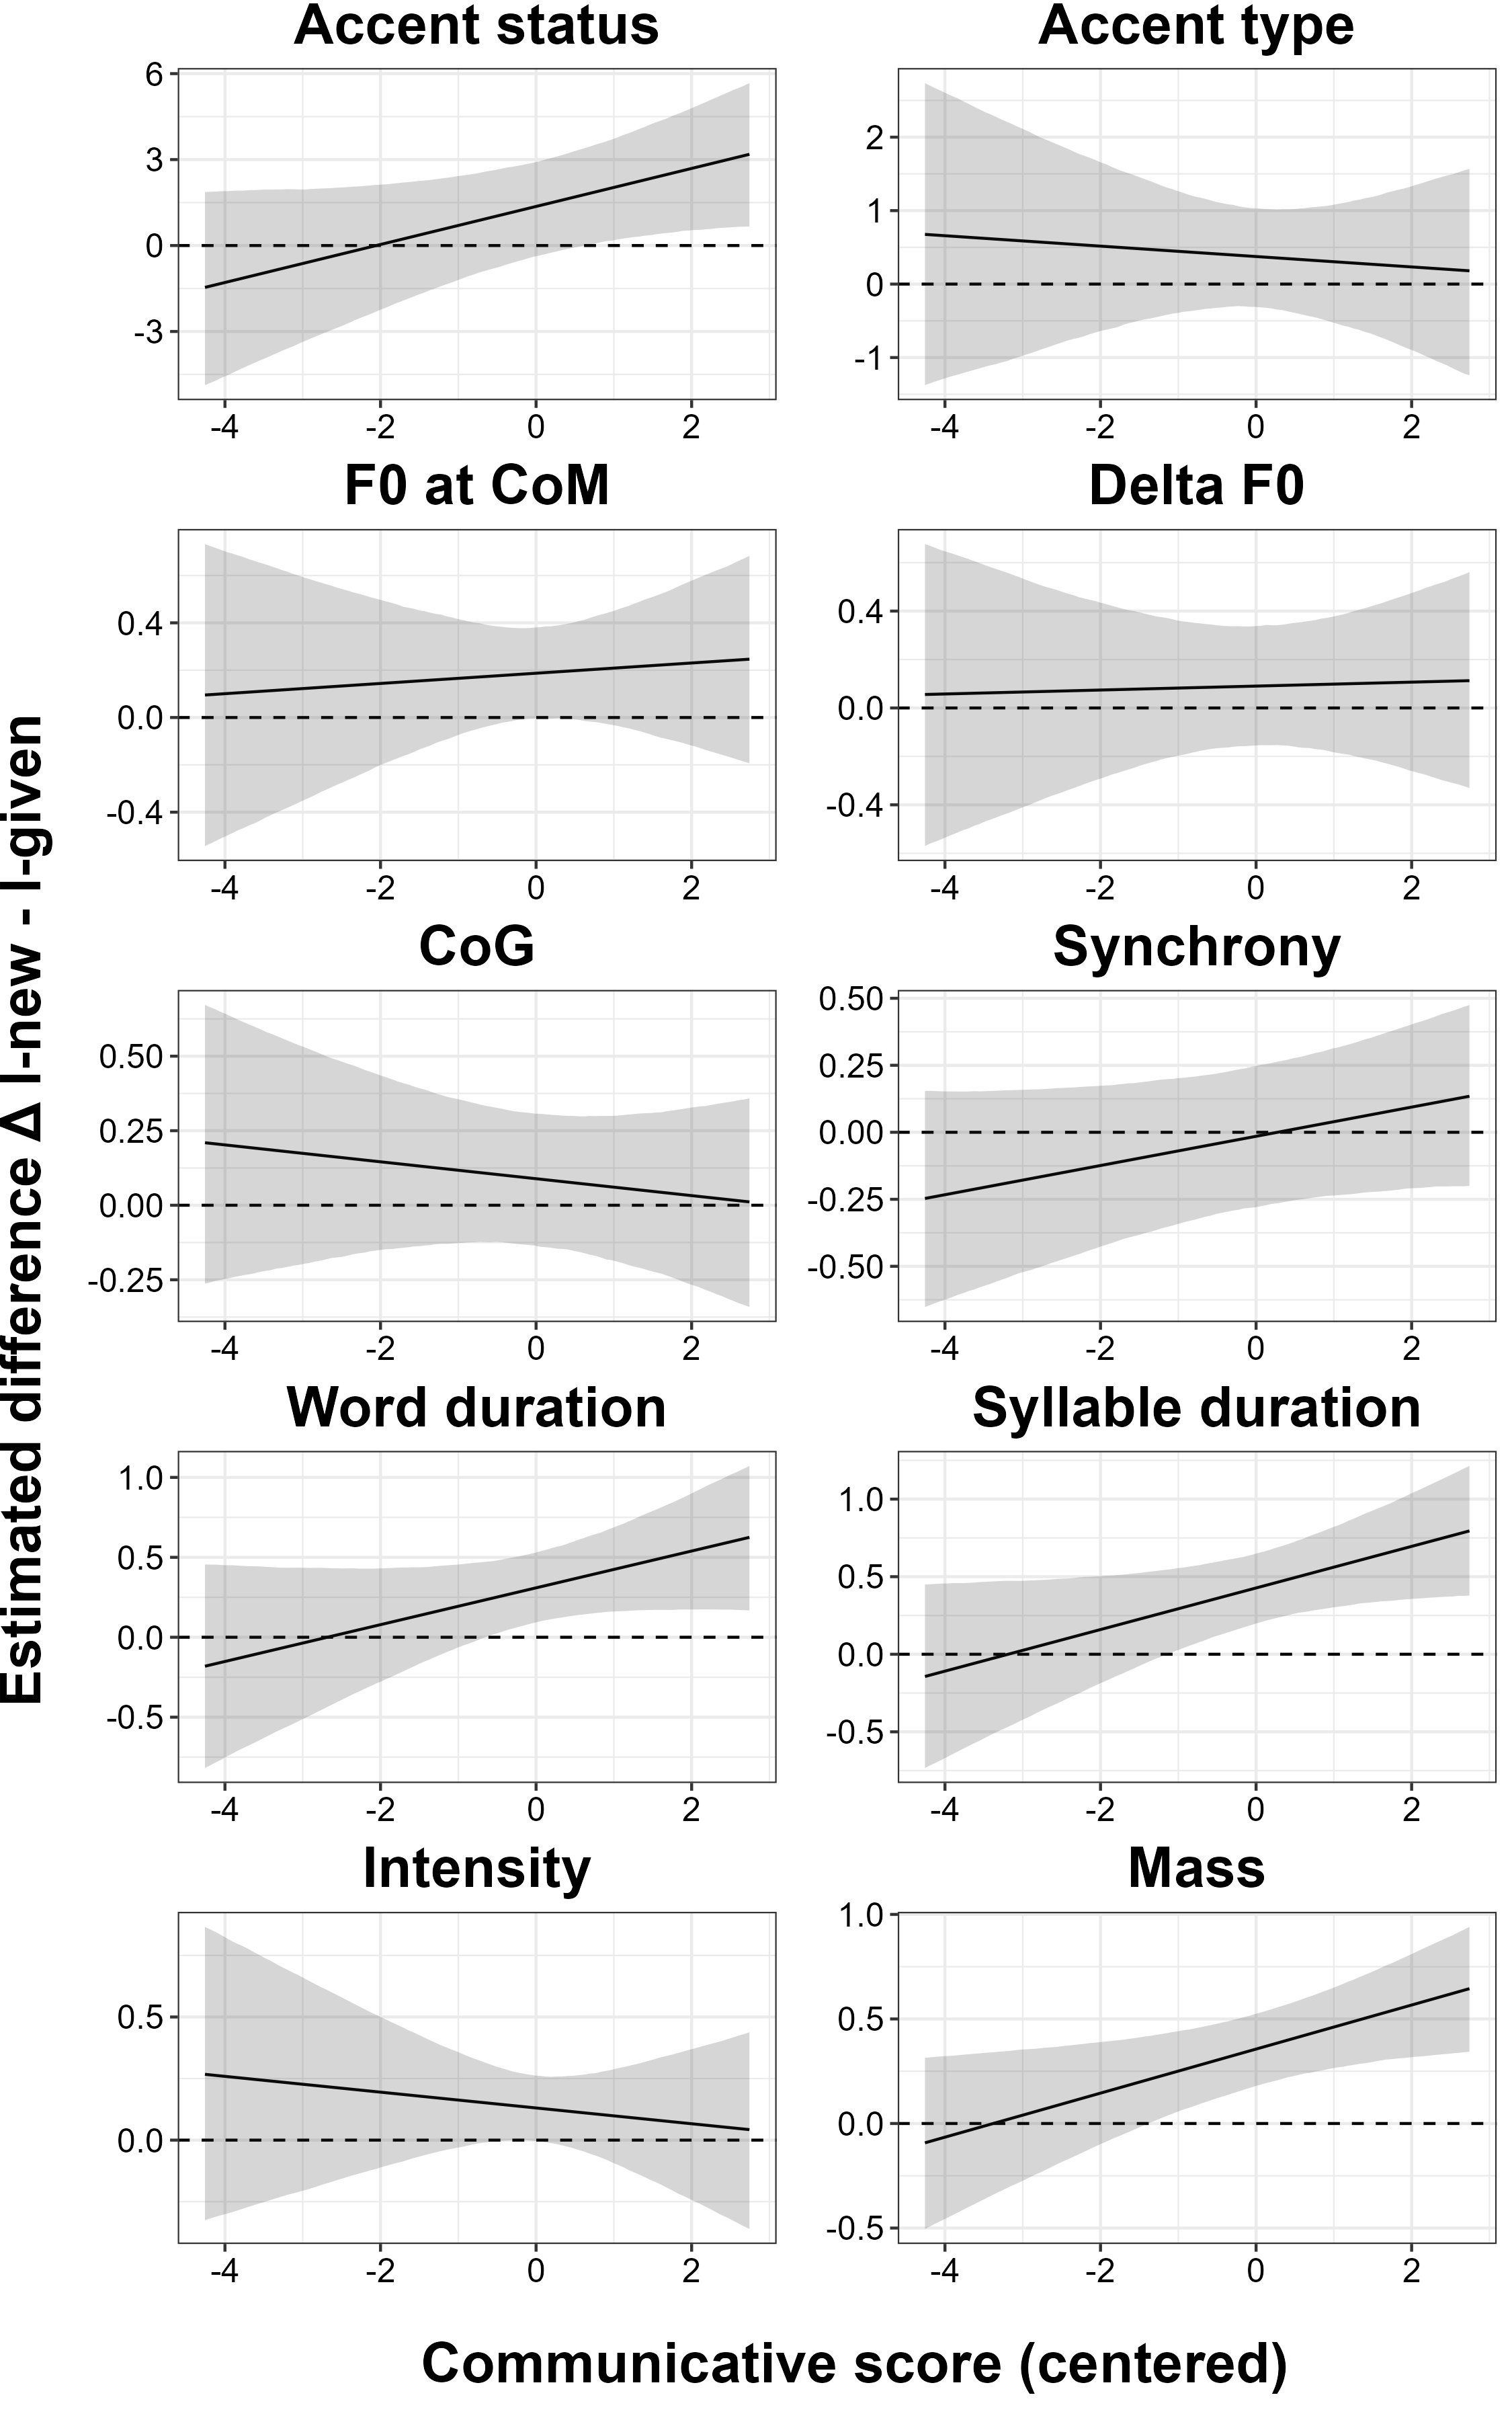
\includegraphics[scale = 0.45]{interactions_lexical-givenness}
	\caption{Estimated differences between lexically new and given referents and 90\% CrIs as a function of communicative score for all parameters.}
	\label{fig:interactions_lexical-givenness}
\end{figure}

Figure \ref{fig:interactions_lexical-givenness} shows the estimated differences between l-new and l-given referents and 90\% CrIs as a function of communicative skill for accent status, accent type, and all eight continuous prosodic parameters. In four parameters (i.e., accent status, word duration, syllable duration, and periodic energy mass), the difference between l-new and l-given referents clearly increases with higher communicative skill to the extent that only speakers with higher communicative skill appear to reliably mark a difference between them. That is, speakers who rated themselves as more communicatively skilled used these parameters more effectively in the expected direction to encode a difference in lexical givenness than speakers with lower communicative skill. The same is true for synchrony, which shows a clearly positive slope, however, the 90\% CrIs include zero for all values of communicative skill. While for F0 at CoM and Delta F0, there barely seems to be a positive moderating effect of communicative skill on the encoding of lexical givenness, accent type, CoG and intensity show a slight decrease in the difference between l-new and l-given with higher communicative skill. However, for all of these latter five parameters, the CrIs include zero for all values of the communicative score variable as can be seen in Figure \ref{fig:interactions_lexical-givenness}. It is thus unlikely that any of the speakers use accent type, F0 at CoM, Delta F0, CoG, synchrony or intensity to encode lexical givenness regardless of their communicative skill.

In Figure \ref{fig:interactions_referential-givenness}, the interactions between referential givenness and communicative skill are plotted. Here, we can generally observe the opposite trend to lexical givenness: Speakers identifying as more communicatively skilled make less of a distinction in the expected direction between r-new and r-given referents in six out of the ten prosodic parameters (accent status, accent type, F0 at CoM, Delta F0, intensity, and periodic energy mass). Only in word and syllable duration do we observe the expected positive slope from lower to higher communicative skill. CoG and synchrony also display negative slopes, however here these lead to a larger difference between r-new and r-given referents for communicatively more highly skilled individuals, albeit in an unexpected direction. 

\begin{figure}
		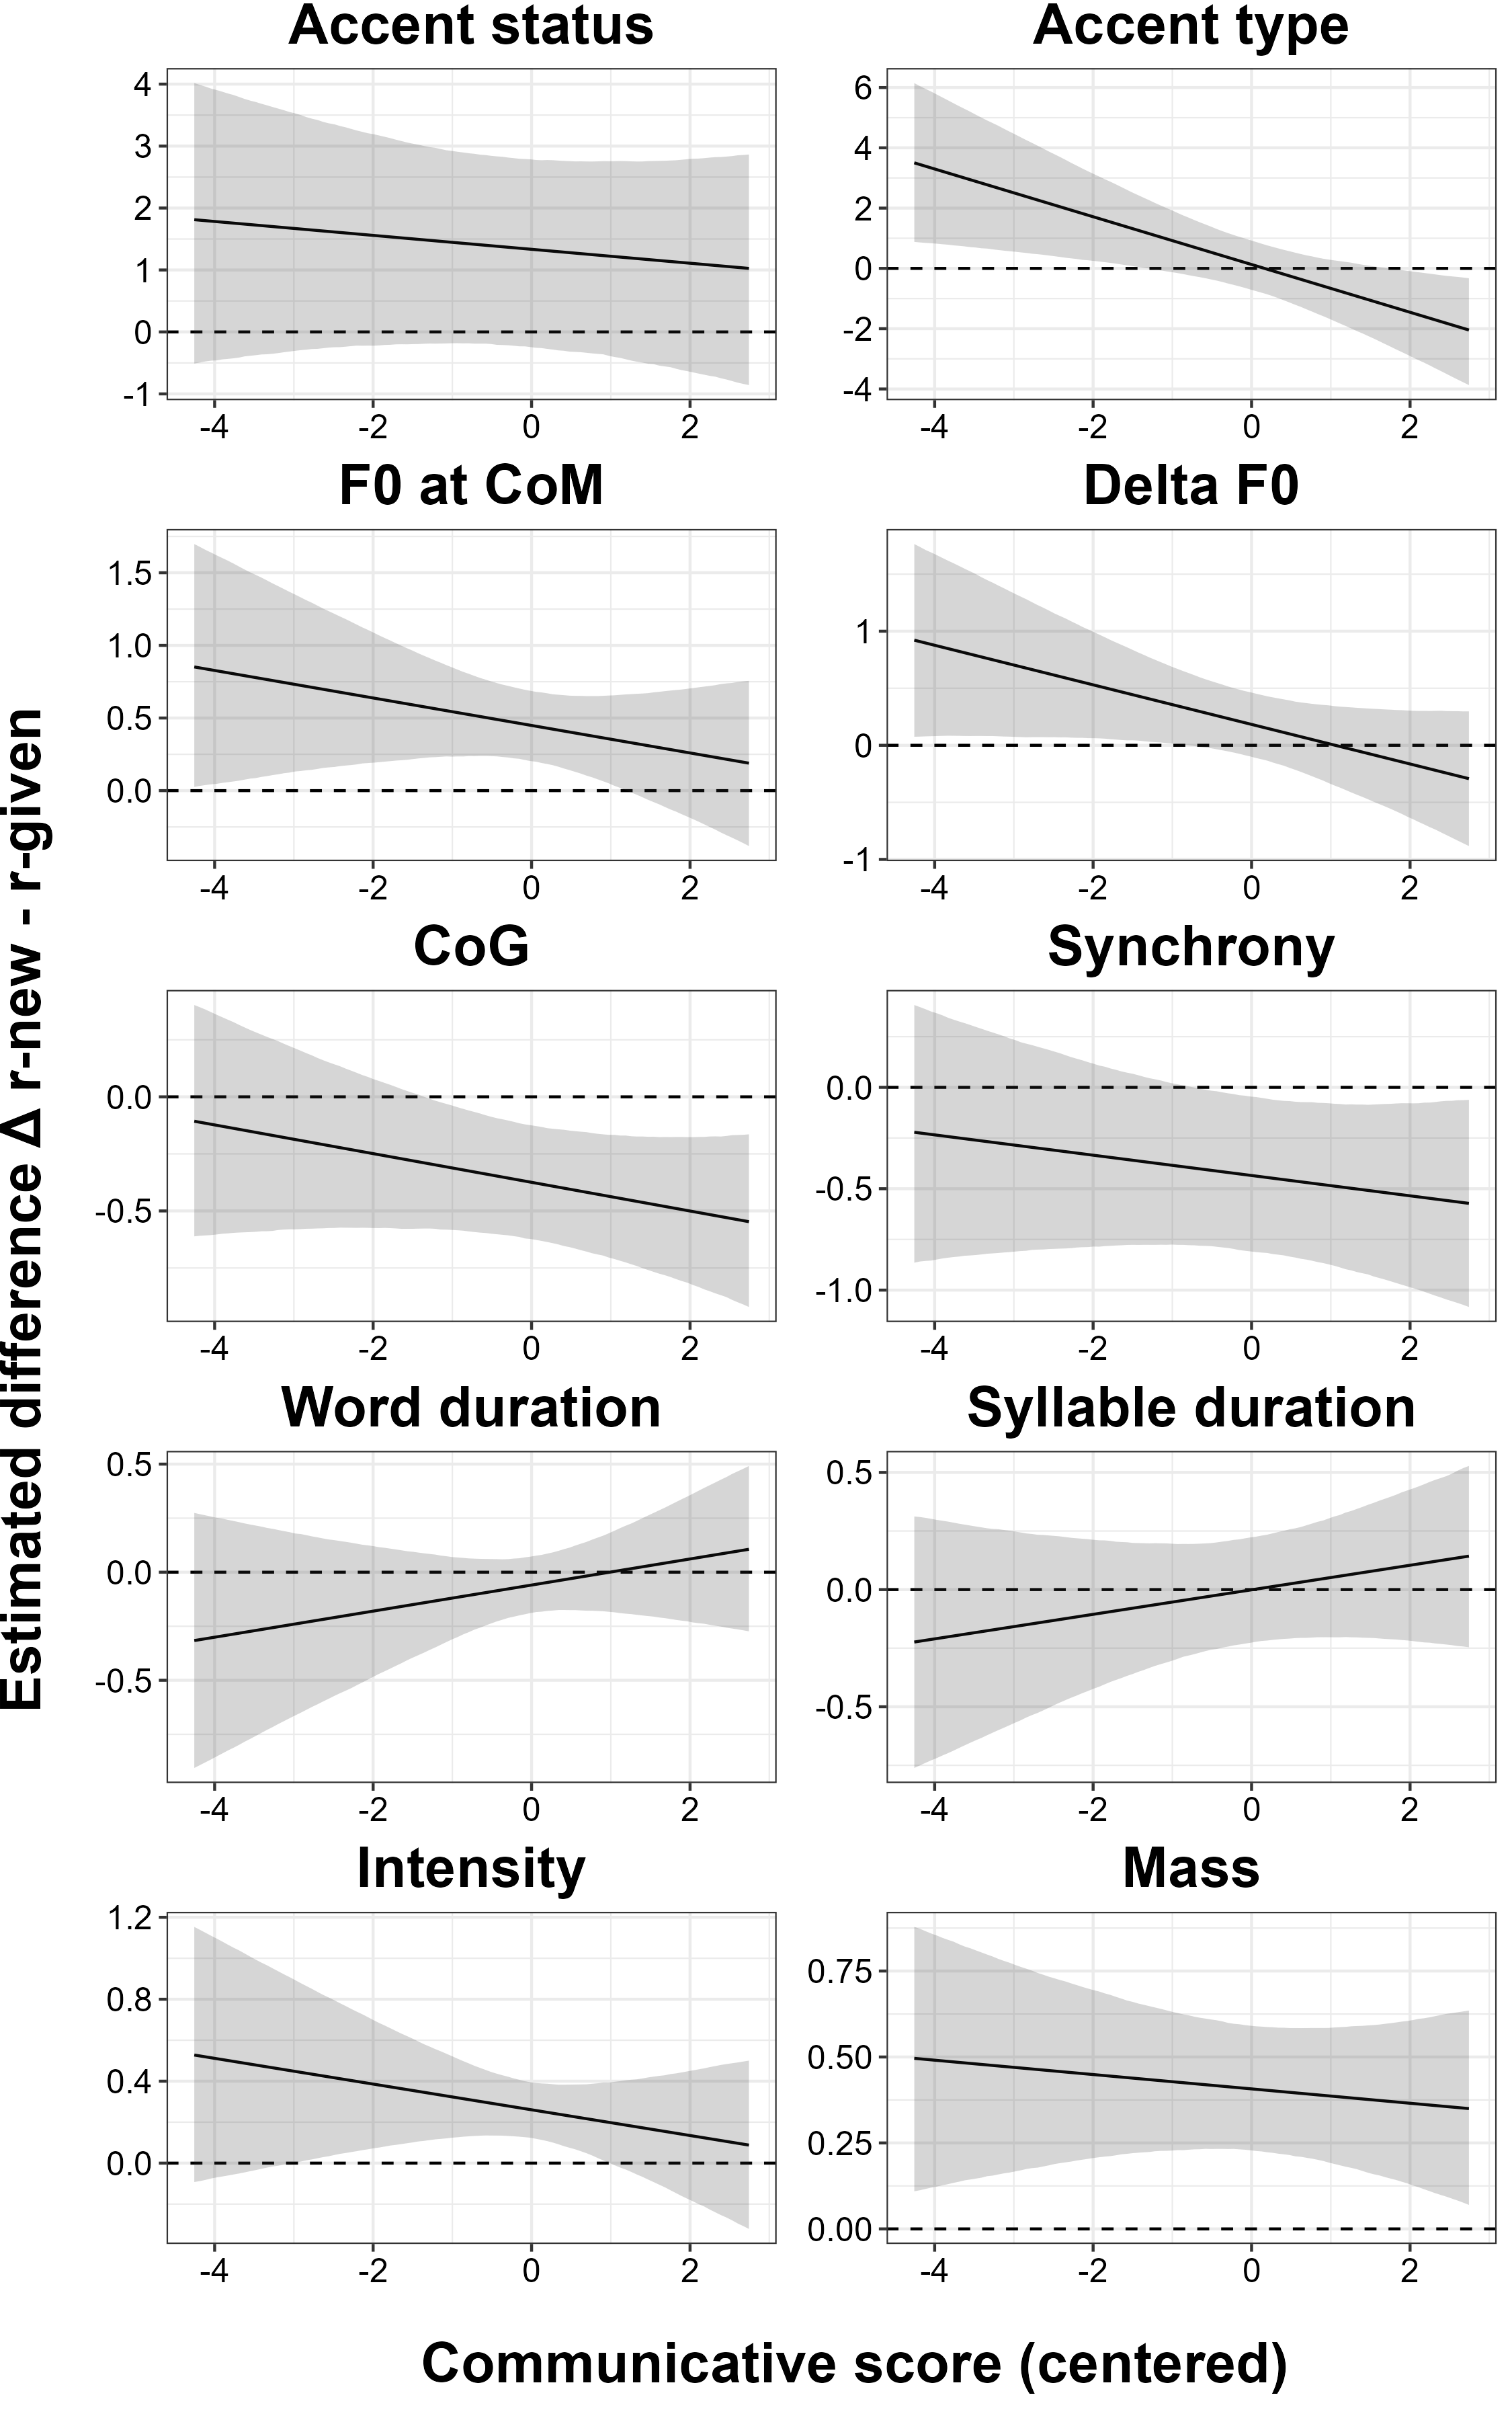
\includegraphics[scale = 0.45]{interactions_referential-givenness}
	\caption{Estimated differences between referentially new and given referents and 90\% CrIs as a function of communicative score for all parameters.}
	\label{fig:interactions_referential-givenness}
\end{figure}

For the encoding of grammatical role, there are again larger positive differences for higher communicative scores in the parameters accent status, word duration, syllable duration, and periodic energy mass and a larger negative difference for CoG (see Figure \ref{fig:interactions_gramm-role}). For the remaining parameters, the moderating effect of communicative skill is relatively subtle as indicated by the flatter slopes in the plots and more extensive overlap between the CrIs and the dashed horizontal zero line. 

\begin{figure}
		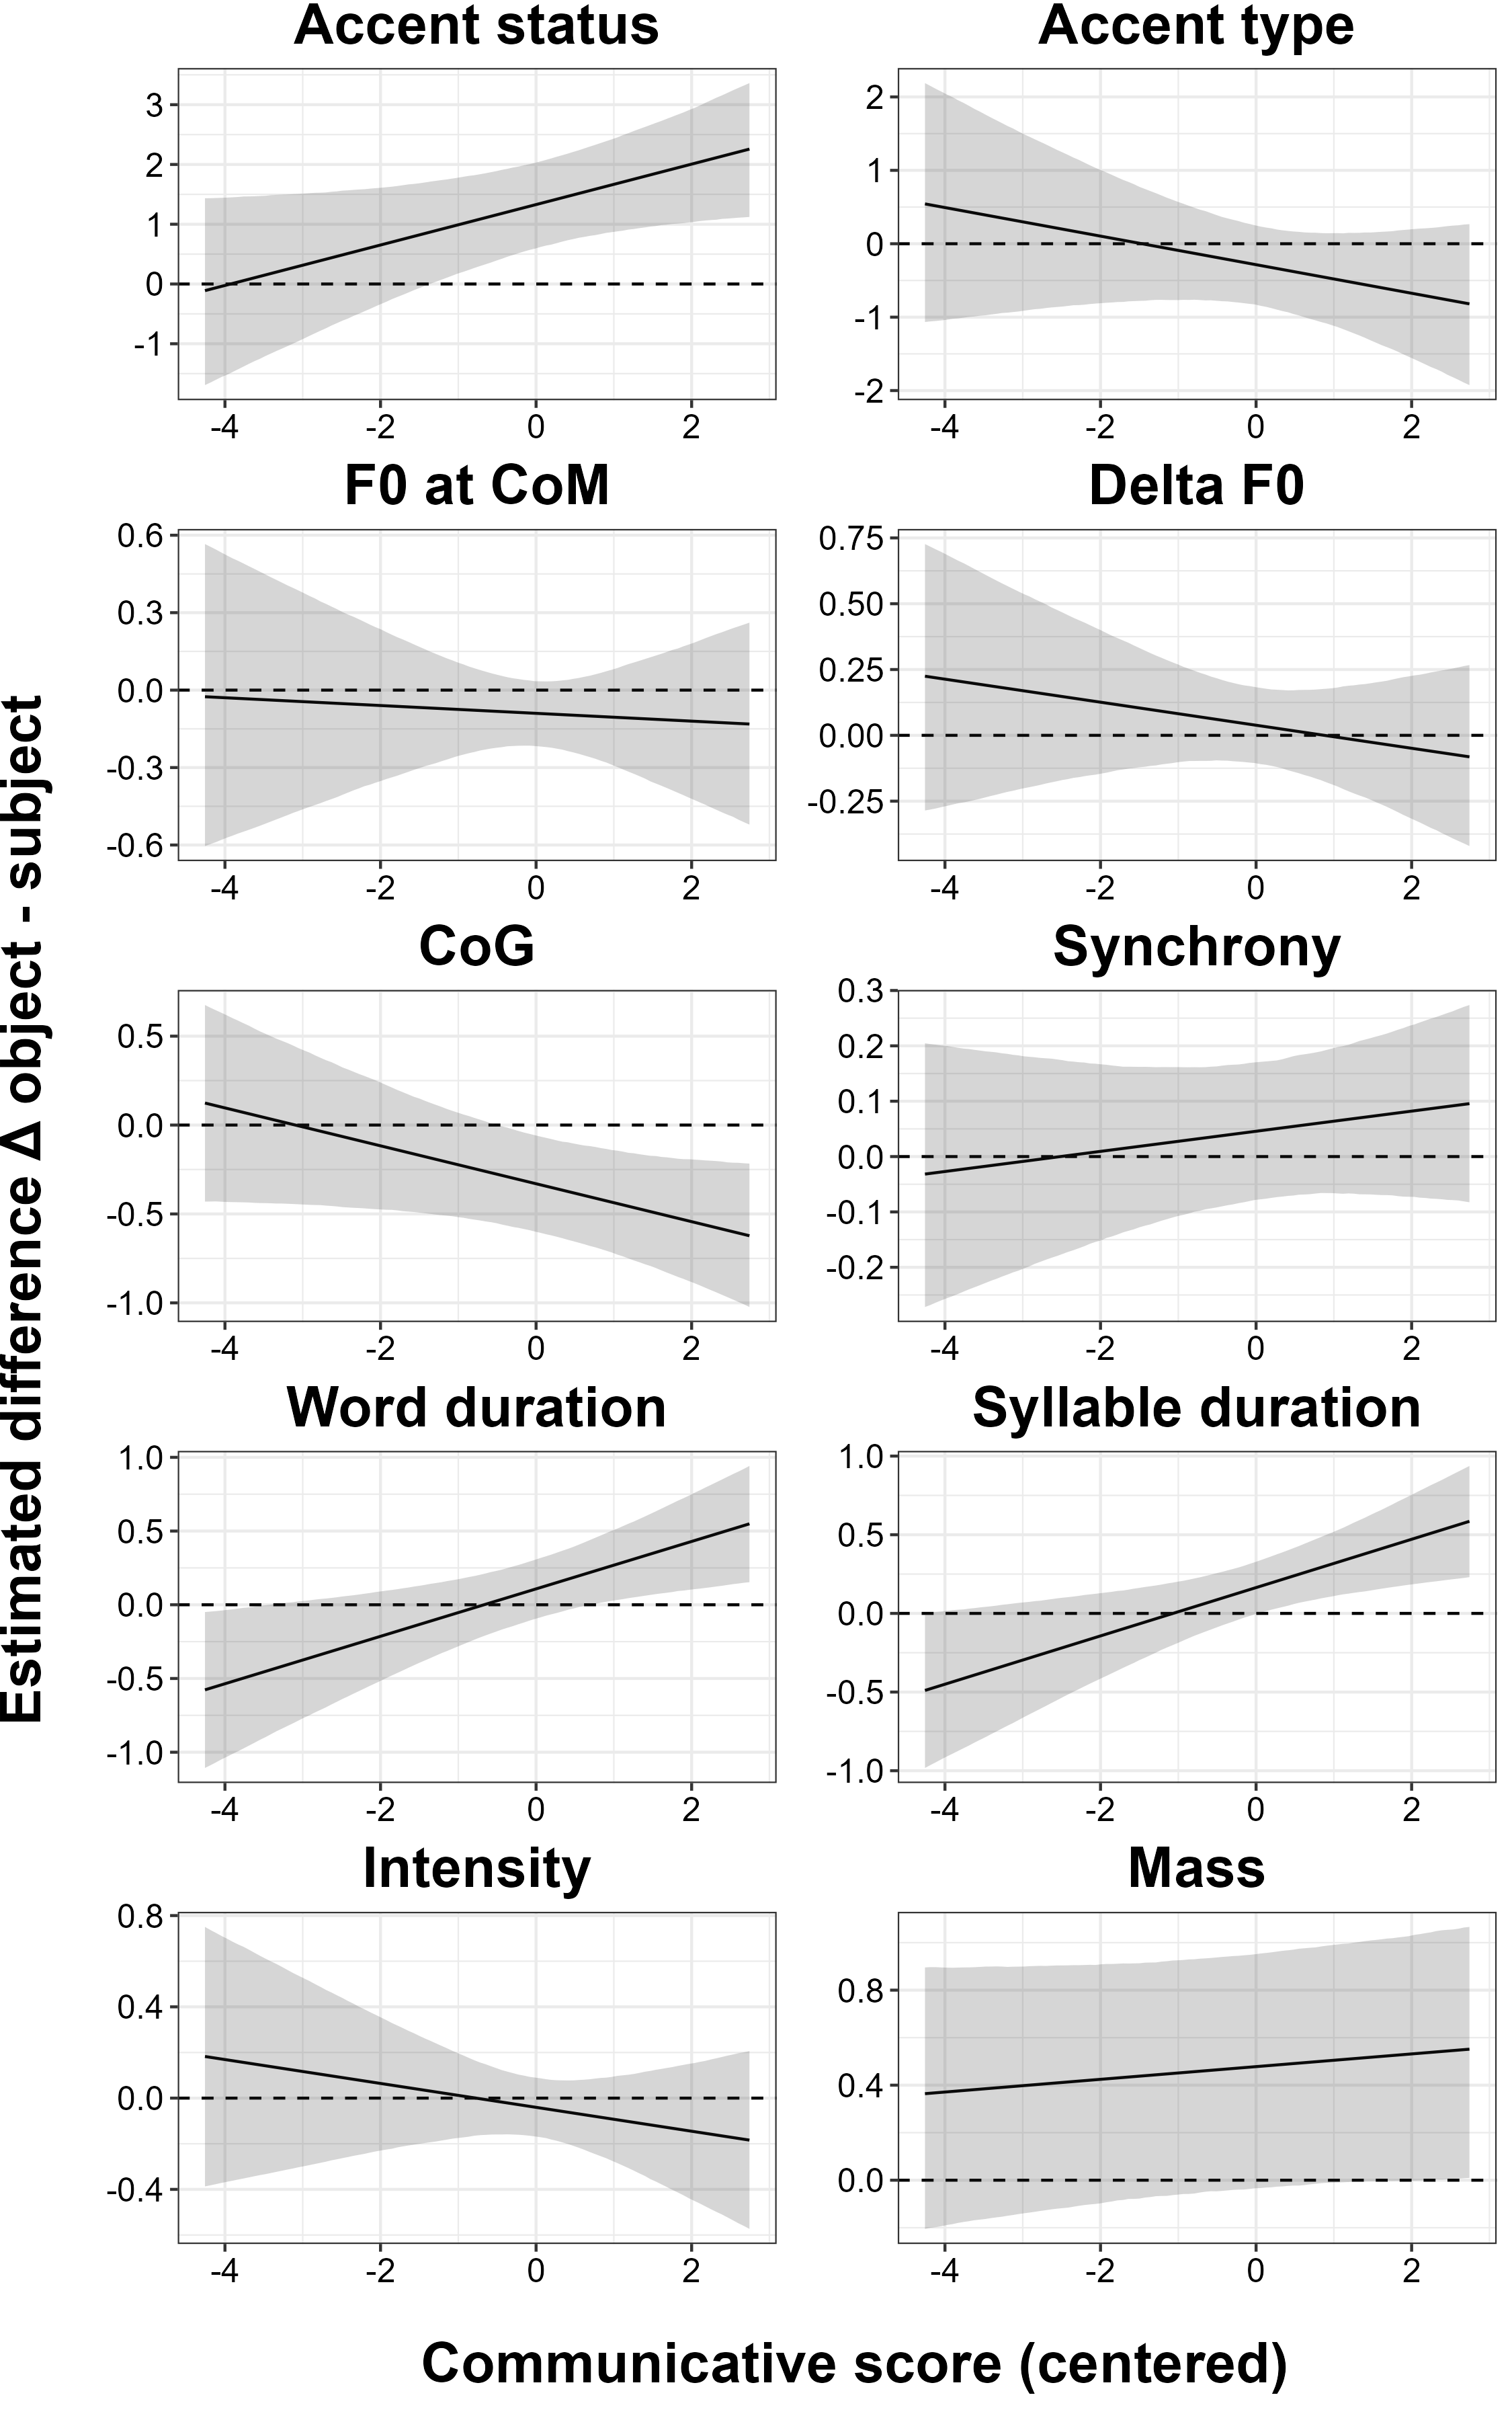
\includegraphics[scale = 0.45]{interactions_grammrole}
	\caption{Estimated differences between grammatical objects and subjects and 90\% CrIs as a function of communicative score for all parameters.}
	\label{fig:interactions_gramm-role}
\end{figure}

Finally, in the encoding of sentence position, differences between initial and medial words are larger for higher communicative scores in F0 at CoM, Delta F0, CoG, synchrony, intensity, and periodic energy mass (see Figure \ref{fig:interactions_position}). For word and syllable duration, this effect is reversed. However, slopes appear to be relatively flat for most prosodic parameters, especially accent status and accent type, with intensity constituting the most notable exception, i.e., the strongest effect of communicative skill. 

\begin{figure}
		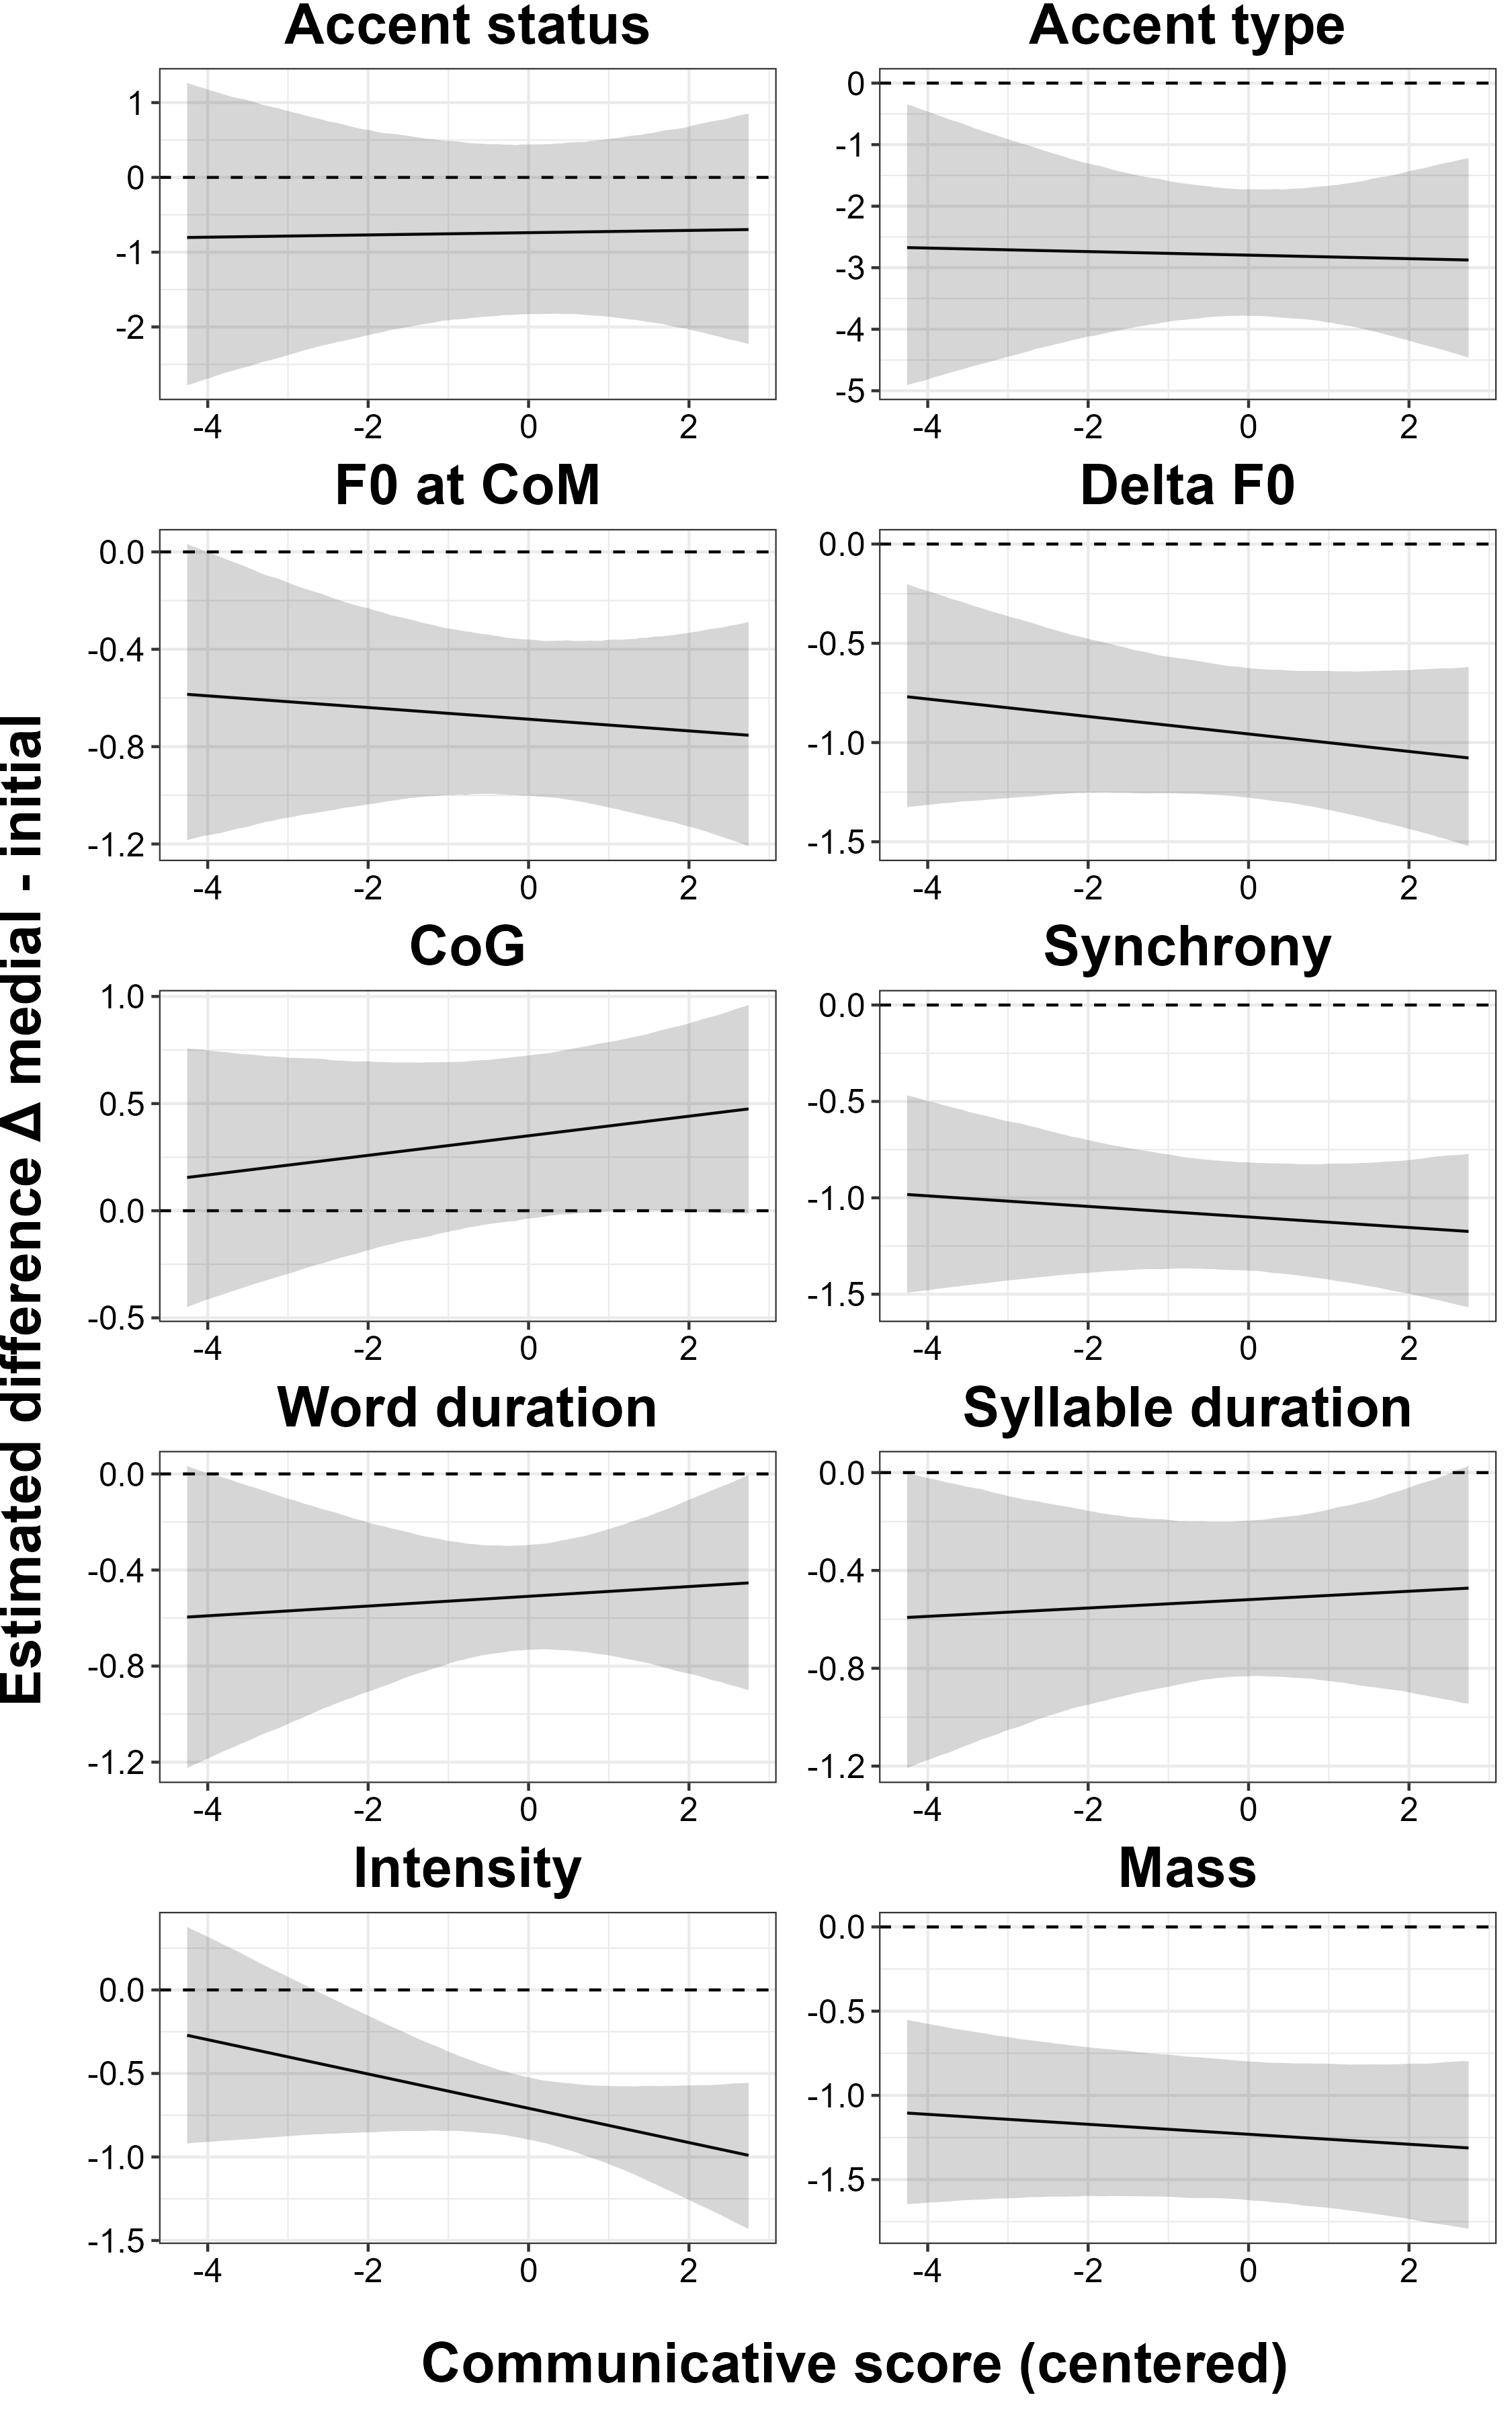
\includegraphics[scale = 0.45]{interactions_position}
	\caption{Estimated differences between words in initial and medial position and 90\% CrIs as a function of communicative score for all parameters.}
	\label{fig:interactions_position}
\end{figure}

\section{Interim discussion} \label{sec:Production2 discussion}

In this study, we investigated the effects of lexical and referential givenness, grammatical role, and sentence position on prosodic prominence production. All four factors were found to influence prominence across speakers. The strongest effect was observed for sentence position, with initial constituents in an utterance generally being produced more prominently than medial target words, more specifically, with more prominent pitch accent types, higher and more steeply rising F0, longer duration, and higher intensity. This result reinforces the importance of an utterance-initial accent in contributing to a rhythmical frame \citep{baumannInfluenceInformativenessProsody2021} and is consistent with Bolinger's (\citeyear{bolingerIntonationItsParts1986}) idea of an \textit{Accent of Power}, which is often placed towards the beginning of an utterance. With regard to information status, our findings confirmed that both the lexical and the referential level influence prosodic prominence \citep{baumannReferentialLexicalGivenness2012, baumannCoreferenceLexicalGivenness2013}. Lexically new as opposed to given target words were reliably marked by longer duration and higher periodic energy mass, but also exhibited strong tendencies to be produced with more nuclear accents and higher F0 and intensity. Referential newness was reliably encoded by higher F0, intensity, and periodic energy mass compared to referential givenness. Finally, grammatical objects were produced with more nuclear accents than subjects, however, the continuous prosodic parameters were least affected by grammatical role out of the four manipulated factors.

On the individual speaker level, we observed different strategies in the prosodic marking of lexical and referential givenness, grammatical role, and sentence position. Of these four factors, the encoding of lexical givenness was least variable in the sense that the cluster analysis revealed only two strategies, which differed only minimally. One cluster encoded the l-new versus l-given contrast slightly more strongly than the other, especially in the prosodic parameters related to timing and intensity. The two strategies we observed for the encoding of referential givenness were more distinct. Here, one cluster relied more on F0 shape and alignment to mark a difference between r-new and r-given referents, while the other cluster used F0 scaling. This observation is reminiscent of a finding by \citet{niebuhrAreThereShapers2011} that German speakers differ in whether they rely more on alignment or scaling to distinguish between different pitch accent types.

Grammatical role was marked less strongly than lexical and referential givenness overall, however, the clustering into three groups appeared to be most stable of all four factors under investigation with the highest average silhouette width. Clusters differed in which cue most reliably encoded grammatical role, with one cluster relying most on CoG and the other two on periodic energy mass. The former cluster additionally made use of periodic energy mass to about the same extent as the other two, leading to a stronger, more redundant encoding of grammatical role in these speakers. These observations show that while averaged group-level results do not reveal any strong tendencies (at least in the continuous parameters), the prosodic productions of individual speakers can be influenced by grammatical role, although this influence manifests in different prosodic parameters. By contrast, sentence position overall was most strongly marked with large differences between initial and medial position for all prosodic parameters and in fact, every single speaker exhibited this trend in at least some of the parameters. Nevertheless, the encoding of sentence position gave rise to the highest number of different strategies as per the cluster analysis. For two clusters, Delta F0 was the most important parameter, for the others it was periodic energy mass. There were also differences in the strength and redundancy of encoding across the clusters, with two of the clusters modifying every parameter. Thus, no matter if the results across speakers indicate a strong overall effect (as for sentence position) or a weak overall effect (as for grammatical role), different speaker-specific strategies may hide under the cover of those general tendencies. To achieve high descriptive adequacy of the relation between prosody and other linguistic dimensions, it is therefore important to consider results below the group level.

To summarize, we found different degrees of variability in the encoding of several semantic-pragmatic and syntactic factors via continuous phonetic parameters. As in the previous production study presented in Chapter \ref{ch:Production I} and similar to previous findings \citep[e.g.,][]{cangemiListenerSpecificPerceptionSpeakerSpecific2015, ouyangIndividualDifferencesProsodic2015, severijnenYourVOORnaamNot2024}, this variability is evident in the strength of encoding of the factors under investigation and the types of parameters used.

With regard to the role of the phonological categories accent status and accent type in the encoding of the different semantic-pragmatic and syntactic factors, we often observed a compensatory behavior at the individual level. Particularly in the marking of referential givenness, grammatical role, and sentence position, speakers using accent status to mark these contrasts were less likely to rely on accent type and vice versa, speakers making use of accent type were less likely to also use accent status. This asymmetry has also been observed in the previously presented production study in Chapter \ref{ch:Production I}. Speakers are thus able to exploit the independency of tune and metrical structure that is postulated by the autosegmental-metrical model \citep[e.g.,][]{laddIntonationalPhonology2008} to encode different linguistic contrasts. This can be regarded as prosodic cue trading not just on a phonetic level as has previously been described by \citet{severijnenYourVOORnaamNot2024} but also on a phonological level. We will return to this point in Chapter \ref{ch: general discussion}.

In this study, deaccentuation of the target word was possible (in the medial position) but rare, only attested in five speakers.\footnote{Deaccentuation may be more frequent in the data than these results suggest, but the difference between a prenuclear accent and deaccentuation is difficult to identify for annotators, especially in this position.} What may ultimately be more important for the information-structural interpretation of utterances than accentuation versus deaccentuation is the structural prominence \textit{relation} between two constituents \citep[e.g.,][]{libermanIntonationalSystemEnglish1975, laddIntonationalPhonology2008, laddProsodicProminenceLanguages2023}. This is particularly relevant for referential givenness, where accent status was more consistently used as a prominence cue across speakers than for lexical givenness. In utterances with referentially new target words, the target word and following verb typically formed a strong-weak pattern, with the target word receiving a nuclear accent and the verb being deaccented. When the target word was referentially given, the pattern was reversed to weak-strong, with the verb receiving the nuclear accent (see also analysis in \citealt{baumannBoostingInhibitingHow2024}). The \textit{weak} target word may either be deaccented or receive a prenuclear accent, but in both cases, the strength relation remained the same. In fact, out of the five speakers that produced deaccented target words, three were among the least consistent users of accent status as a cue to referential givenness.

One reason for the manifestation of different individual strategies that has been considered especially in prominence perception studies is communicative skill. Generally, listeners with higher communicative skill have been found to be more adept at perceiving prominence differences than listeners with lower communicative skill \citep{bishopPhonologyPhoneticsSignalextrinsic2020, orricoInfluenceEmpathyAutisticlike2023}. Analogously, we expected speakers with higher commmunicative skill to encode semantic-pragmatic and syntactic contrasts more strongly than speakers with lower communicative skill. In our data, we observed this expected mediating effect (on several prosodic parameters) for lexical givenness, grammatical role, and sentence position. However, referential givenness seemed to be encoded more clearly by speakers with lower communicative skill, which is contrary to our expectations and the findings by \citet{bishopPhonologyPhoneticsSignalextrinsic2020} and \citet{orricoInfluenceEmpathyAutisticlike2023}. 

That individual speakers should behave differently in their encoding of lexical givenness on the one hand and referential givenness on the other hand may be due to the different sources of these two variables. Referential givenness describes the relation between entities (i.e., creatures, things, states or events) in the situational or textual discourse context, while lexical givenness is determined by the previous occurrence or absence of a word or concept \citep{baumannCoreferenceLexicalGivenness2013}. In fact, our findings are partially in line with Turnbull's (\citeyear{turnbullListenerorientedPhoneticReduction2019}), who found that speakers with lower communicative skill encoded semantic-pragmatic predictability more strongly prosodically than speakers with higher communicative skill. Semantic-pragmatic predictability is comparable to referential givenness in our study. However, \citet{turnbullListenerorientedPhoneticReduction2019} found no mediating effects of communicative skill on the encoding of second mention reduction, which may be claimed to fall within the scope of lexical givenness.
 
The interaction of communicative skill and referential givenness is unexpected in the context of previous perception studies that report a higher sensitivity to the mapping of prosody to meaning in communicatively more skilled listeners \citep{bishopPhonologyPhoneticsSignalextrinsic2020, orricoInfluenceEmpathyAutisticlike2023}. In line with these findings, we assumed that highly communicatively skilled speakers should be able to anticipate the higher activation cost demanded of the listener by an r-new referent \citep{chafeDiscourseConsciousnessTime1994} and thus produce a stronger prosodic contrast to clearly mark the distinction between r-new and r-given. It appears that instead, such speakers underestimated this activation cost and generally produced a weaker contrast. A potential explanation is that the communicatively skilled speakers relied more on the morphosyntactic marking of r-givenness, since r-new referents were preceded by an indefinite article, while r-given referents were preceded by a definite article, making an additional prosodic marking obsolete. 

Like \citet{turnbullListenerorientedPhoneticReduction2019}, we also observed inconsistent mediating effects of communicative skill on different prosodic parameters. However, these inconsistencies were at least partially systematic: For lexical givenness and grammatical role, prosodic variables related to timing, such as accent status, word and syllable duration, and periodic energy mass, were most affected by communicative skill. For referential givenness, the parameters describing the alignment and scaling of the F0 contour (i.e., accent type, F0 at CoM, Delta F0, CoG, and synchrony) were modulated to a larger extent by communicative skill. Nevertheless, it remains unclear at this point why communicative skill should mediate the use of timing but not F0 in the case of lexical givenness and F0 but not timing in the case of referential givenness. This remains an issue for further investigation in future studies.

Our findings are limited by the measure of communicative skill we employed, which is very coarse-grained as it relies on the self-assessment of the participants. Other instruments assessing different aspects of communicative skill could yield more precise results that better relate to speech production in general and the different dimensions of givenness in particular. For example, \citet{orricoInfluenceEmpathyAutisticlike2023} employed a questionnaire to measure emotional and cognitive empathy \citep{baron-cohenEmpathyQuotientInvestigation2004} and found that empathy affects the processing of contrastive focus. Furthermore, we considered relatively few participants (especially compared to perception studies), and most of them had high communicative skill, which limits the generalizability of our findings. 

Previous studies investigating individual variability often only looked at one factor to be encoded prosodically at a time, e.g., focus type in \citet{cangemiListenerSpecificPerceptionSpeakerSpecific2015}. This study finds that some speakers are more successful at distinguishing between focus types than others. A reasonable deduction could thus be made that there are ``good" and ``bad" communicators, i.e., speakers who more or less effectively use prosody to encode meaning. By considering several semantic-pragmatic and syntactic factors to be encoded by prosody in the same study, we contribute more insight to the idea of strong versus weak encoders. In particular, this study shows that speakers who strongly mark lexical givenness prosodically are not at the same time the stronger encoders of referential givenness (and grammatical role and sentence position). In the interactions with communicative skill, it is evident that the encoding of lexical and referential givenness may require different skills or traits of speakers. However, to lend more insight into individual variability and its impact on communicative success, a perception study is needed to disentangle the effects of semantic-pragmatic, syntactic, and prosodic cues on the interpretation of prominence. This is the main objective of the next Chapter. 
